\section{Effect of Copy Number Alterations on Gene Expression}
It has been reported in literature that CNAs can promote tumour progression by altering gene expression levels \citep{pmid12297621, pmid17289997,  pmid22522925, pmid32024838}. Here, we utilise differential gene expression analysis (DGEA) to explore the impact of CNAs on gene expression. DGEA identifies differences in gene expression comparing conditions or states, e.g. healthy/disease or treatment/control states, allowing identification of differentially expressed genes (DEGs) and biological pathways that may be perturbed. DGEA has been used to compare gene expression patterns in breast cancer facilitating the formation of the IntClust molecular classification and a number of prognostic and predictive assays \citep{pmid22522925, pmid28882552}. 

Microarrays and RNA sequencing are the two most common technologies used to study transcriptional activity \citep{pmid10851158, pmid19015660}. Microarrays contain thousands of probes, usually oligonucleotide or complementary DNA probes, anchored to a glass slide at defined positions. Fluorescently labelled RNA or DNA in observed tissue samples hybridise to the probes present on the array and hybridization intensities measured for each probe are converted to a quantitative read-out of relative gene expression levels. This allows simultaneous measurement of the expression level of thousands of genes and direct comparison of different tissue samples via different fluorescent labelling on a single hybridization assay \citep{pmid10851158, pmid17660860}. There are numerous microarray platforms available for carrying out gene expression analysis. In the METABRIC study \citep{pmid22522925}, the microarray platform used for measuring gene expression was the HumanHT-12 BeadChip (v3) produced by Illumina, which supports highly efficient whole-genome expression studies and expression-based quantitative trait loci studies. This RNA microarray contains more than 48,000 probes that provide genome-wide transcriptional coverage of more than 25,000 RefSeq and UniGene annotated genes, including well-characterised genes, gene candidates, and splice variants \citep{Illumina}. Microarrays can be used for other purposes, such as genotyping and for the detection of CNAs. To carry out copy number and genotype analysis in the METABRIC study, the Affymetrix Genome-Wide Human SNP Array 6.0 array was utilised \citep{pmid22522925}, containing over 1.8 million probes, approximately 906,600 probes for single nucleotide polymorphisms (SNPs) and 946,000 probes for the detection of copy number variation. These probes are evenly distributed across the entire genome, facilitating measurement of copy number, allele-specific copy number, and copy number-neutral LOH \citep{Affy}.  

This chapter provides an overview of approaches to DGEA, including a common R programming package limma \citep{pmid25605792}. DGEA is applied to compare gene expression between groups of stratified patients identified as having similarity in survival curves, derived by incorporating the CNA information, in Section \ref{Trees_Arm}, i.e. comparing patients of particular survival tree nodes of interest. DGEA is also applied to compare gene expression between different gene CNA states, i.e. homozygous deletion (-2), hemizygous deletion (-1), diploidy (0), single copy gain (+1) and high-level amplification (+2). To finish, the differentially expressed gene sets emerging from this analysis, are compared to previously defined breast cancer prognostic and predictive gene sets, i.e. Oncotype DX, MammaPrint, Prosigna and BCI, and the molecular classification gene sets, i.e. PAM50 and IntClust. 

\subsection{Differential Gene Expression Analysis using Limma}
Limma is a Bioconductor/R software package that facilitates analysis of data generated from microarray and RNA-sequencing gene expression experiments \citep{pmid25605792}. In its implementation, limma fits a linear model to each gene simultaneously, taking as input a matrix of expression values, with rows corresponding to genes and columns corresponding to RNA samples, and a user-specified model design matrix. These linear models are incredibly flexible, capable of handling complex experimental designs, and can be used to test various hypotheses. In addition, limma can distinguish and estimate different sources of variability, e.g. between genes, between samples, variations in quality of data sources, and technical or biological heterogeneity. Limma applies adjustments for different sources of variability, implementing information borrowing between genes and use of observation weights and variance modelling, enabling robust conclusions for statistical testing, particularly when sample sizes are small. 

A general limma pipeline, for microarray analysis, begins with preprocessing, including background correction and normalisation, followed by creation of the design matrix and generation of array weights. Array weights correspond to the relative reliability of each microarray based on how well the expression values from that array follow the linear model, where arrays that have larger residuals, i.e. larger deviations, are assigned lower weights. The linear model is then fitted for each gene given a series of arrays, with the option to apply array weights. To test specific hypotheses, contrasts are fitted using the model estimates, and log-odds of differential expression, moderated t-statistics, and moderated F-statistic are computed. The moderated statistics borrow information from across genes and samples, facilitated using empirical Bayes methods to obtain posterior variance estimators \citep{pmid16646809}. The resulting estimated variance for each gene is then an informed balance between the gene-wise estimator obtained from the data for that gene alone and the global variability across all genes estimated by pooling the ensemble of all genes. Finally, a number of functions can be used to summarise and visualise the results of the estimated linear models, hypothesis test, and apply p-values adjustments for multiple testing, e.g. topTable and volcano plots. 

The basic limma pipeline, fitted with array weights and applying the same common design matrix for all genes, is used in Section \ref{Sec_limma} to identify up- or down-regulated genes between survival tree nodes. A single design matrix, including the predictor variable indicating survival tree node membership for the individual patient, is defined and applied to every gene in the dataset. The contrast matrix specifies which survival tree node comparisons are of interest. Using the topTable results, a gene is called as differentially expressed if the adjusted p-value is below 0.05 and the absolute log-fold change is above 0.58, i.e. greater than a 1.5-fold change \citep{pmid19176553}.  

In Section \ref{Sec_limma_2}, to model the direct relationship between CNA states and gene expression, a modified limma pipeline allowing a different design matrix to be fitted for each gene is implemented. The modification, and additional tailored R programming, is necessary in this application since a patient's CNA state may differ across genes. In addition, since some genes may not exhibit any CNAs or have very few, resulting in cases where the sample size of the particular CNA state may be too small to support inference, genes not altered with sufficient frequency ($< 1\%$) in the CNA state of interest were filtered out for that comparison only. 

\subsection{Application to METABRIC cohort}
DGEA to compare gene expression between METABRIC patients stratified by the global and chromosome arm CNA metric informed survival profiles was carried out. We first focus on presenting four DGEA applications of interest from the survival trees produced as a result of incorporation of the global CNA metric information and then on presenting three DGEA applications of interest from the survival trees produced as a result of incorporation of the chromosome arm CNA metric information. These survival trees, produced for a range of survival times (DSS, 5- and 10-year DSS) and algorithms (rpart and ctree), were selected for DGEA as they partitioned the METABRIC patients first on PAM50 or IntClust and subsequently on a single global or chromosome arm CNA metric, simplifying comparison and inference. The gene expression data, downloaded from cBioPortal in 2023 and used here, include 18,739 genes for which CNA, gene expression and genomic location data were available. 

\subsubsection{Differential Gene Expression Analysis of Global CNA Metric Survival Tree Nodes}
\label{Sec_limma}
Focusing on the survival trees including PAM50 subtype and the six global CNA Burden metrics as candidate predictors (Figure \ref{fig:DGEA_Global_VP_PAM50}A), the DSS ctree survival tree indicates that for patients within specific PAM50 subypes (Claudin-low and Luminal A), survival profiles could be stratified into two nodes: Node 5 with poorer DSS outcome compared to Node 4 with better DSS outcome, where global CNA Del Burden performed as the classifier into the two nodes, patients with global CNA Del Burden above a value of 18.28\% in Node 5. Applying DGEA to compare gene expression of patients classified into Node 5 (higher GI and lower DSS outcome) and patients classified into Node 4 (lower GI and better DSS outcome), reveals 77 down-regulated genes and 37 up-regulated genes. A number of genes including CXCL10 and CXCL9 are identified as significantly up-regulated in Node 5, while genes including PIP, ANKRD30A, and REEP6, are among those identified as significantly down-regulated in Node 5 compared to Node 4 (Figure \ref{fig:DGEA_Global_VP_PAM50}A).  

The 5-year DSS ctree survival tree (Figure \ref{fig:DGEA_Global_VP_PAM50}B) indicates that for Luminal A patients, survival profiles could be stratified into two nodes: Node 9 with global CNA Del Burden $> 14.55\%$ and poorer DSS outcome, compared to Node 8 with global CNA Del Burden $\leq 14.55\%$ and better DSS outcome. Applying DGEA to compare gene expression of patients classified into Node 9 (higher GI and lower DSS outcome) and patients classified into Node 8 (lower GI and better DSS outcome), reveals 15 down-regulated genes and 4 up-regulated genes. Genes SLC7A5, PITX1 and S100P, are identified as significantly up-regulated in Node 9, while genes PIP, FCGBP and SCUBE2, are among those identified as significantly down-regulated in Node 9 compared to Node 8 (Figure \ref{fig:DGEA_Global_VP_PAM50}B). 

Focusing on the survival trees including IntClust and the six global CNA Burden metrics as candidate predictors, the DSS rpart survival tree (Figure \ref{fig:DGEA_Global_VP_IC}A), indicated that for patients within specific IntClusts (3, 4ER+, 7 and 8), survival profiles could be stratified into two nodes: Node 4 with poorer DSS outcome compared to Node 3 with better DSS outcome, where global CNA burden performed as the classifier into the two nodes, patients with global CNA Burden above a value of 24.90\% in Node 4. Applying DGEA to compare gene expression of patients classified into Node 4 (higher GI and lower DSS outcome) and patients classified into Node 3 (lower GI and better DSS outcome), reveals 13 down-regulated genes and 3 up-regulated genes. Genes UBE2C and S100P, are identified as significantly up-regulated in Node 4, while genes PIP, CYBRD1, IRX2, are among those identified as significantly down-regulated in Node 4 compared to Node 3 (Figure \ref{fig:DGEA_Global_VP_IC}A). 

The 10-year DSS ctree survival tree (Figure \ref{fig:DGEA_Global_VP_IC}B), showed that for patients of certain IntClusts (IntClust 3, 4ER+, 7 and 8), their 10-year survival patterns could be stratified, using global CNA Del Burden, into two nodes: Node 7 with CNA Del Burden $>8.82\%$ and poorer 10-year DSS outcome compared to Node 7, where patients have CNA Del Burden $\leq8.82\%$ and better 10-year DSS outcome. Applying DGEA to compare those with higher deletion burden, Node 7, to lower deletion burden, Node 6, identifies 18 differently expressed genes including UBE2C, PIP, and IRX2 (Figure \ref{fig:DGEA_Global_VP_IC}B).

\vfill
\begin{figure}[H]
\begin{center}
\begin{multicols}{2}
	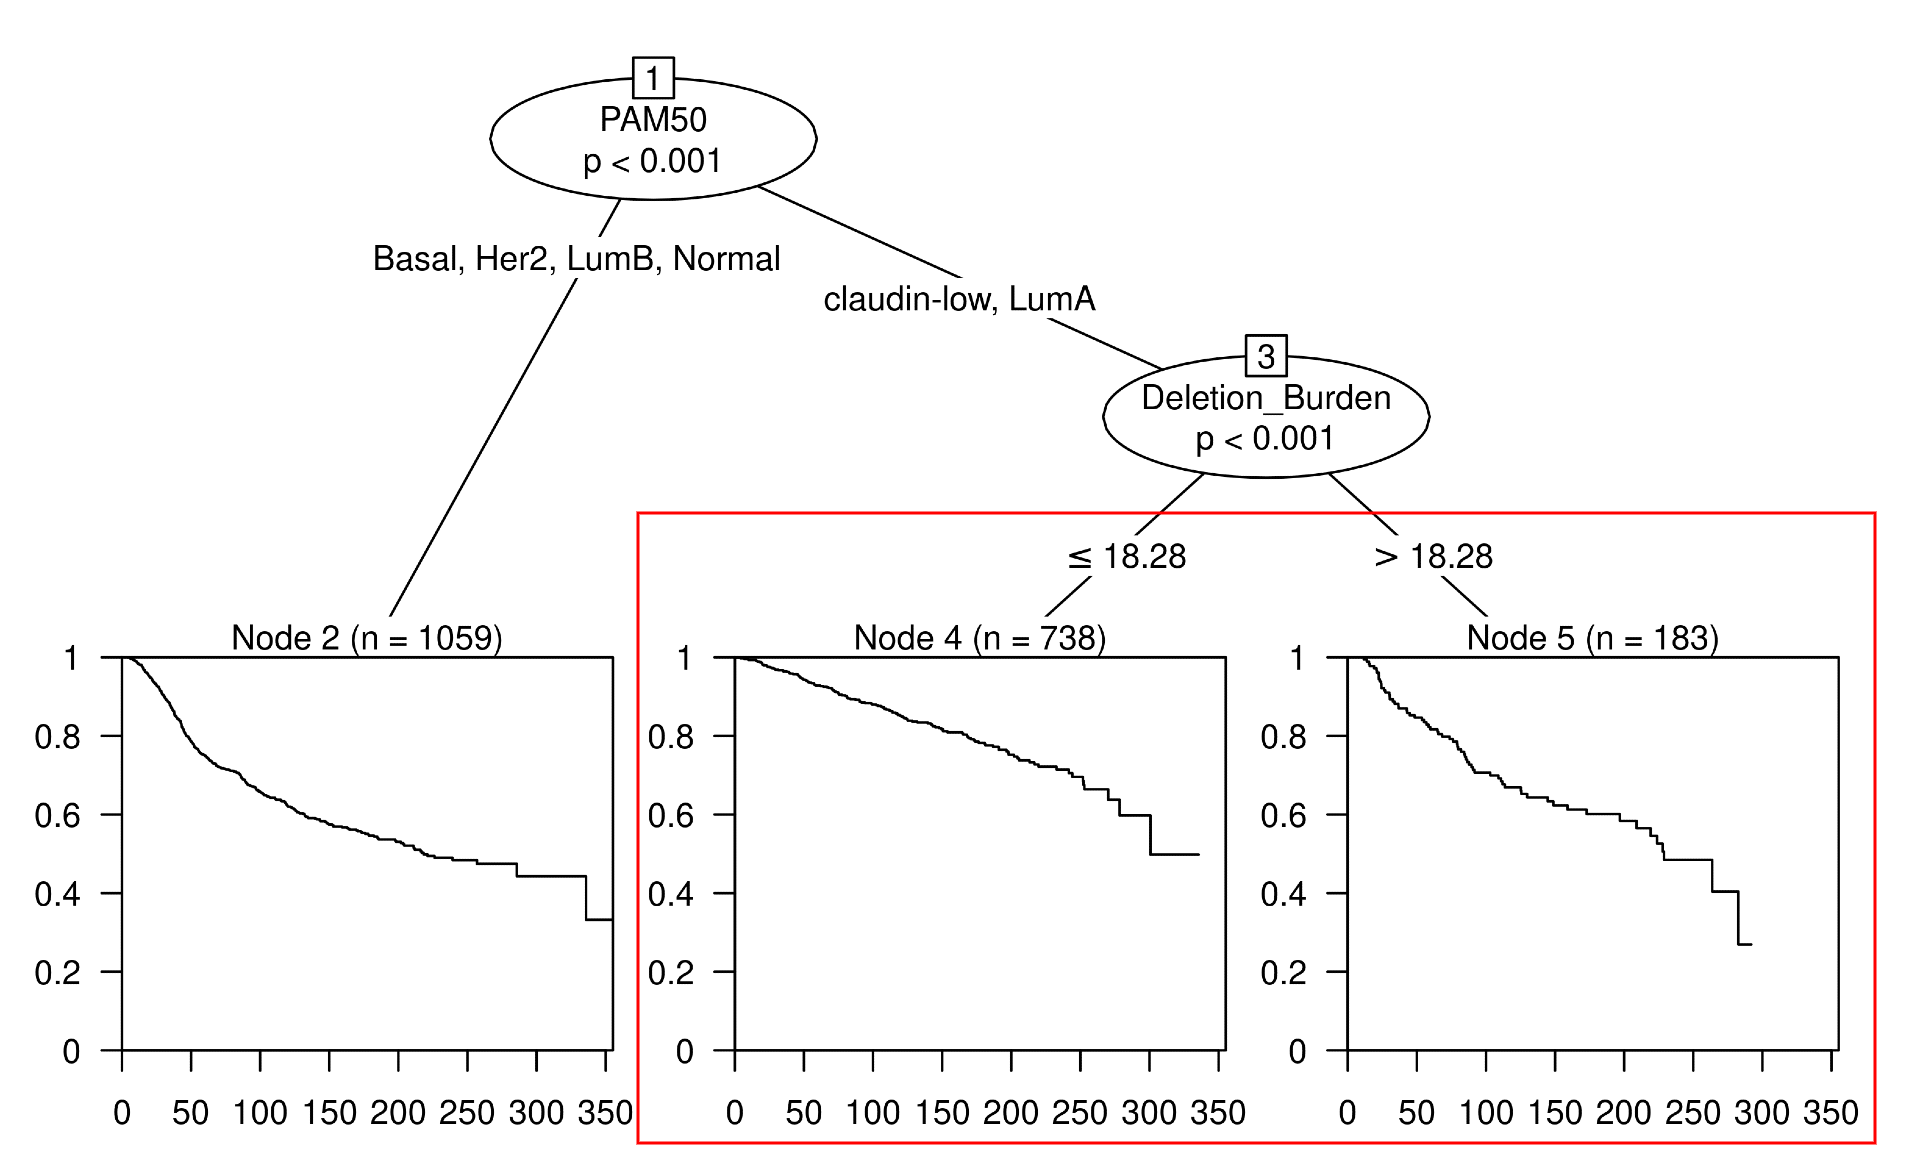
\includegraphics[width=1\linewidth]{../figures/Chapter_4/Ctree_Survival_Burden_DSS_PAM50_Ann.png}\par 
    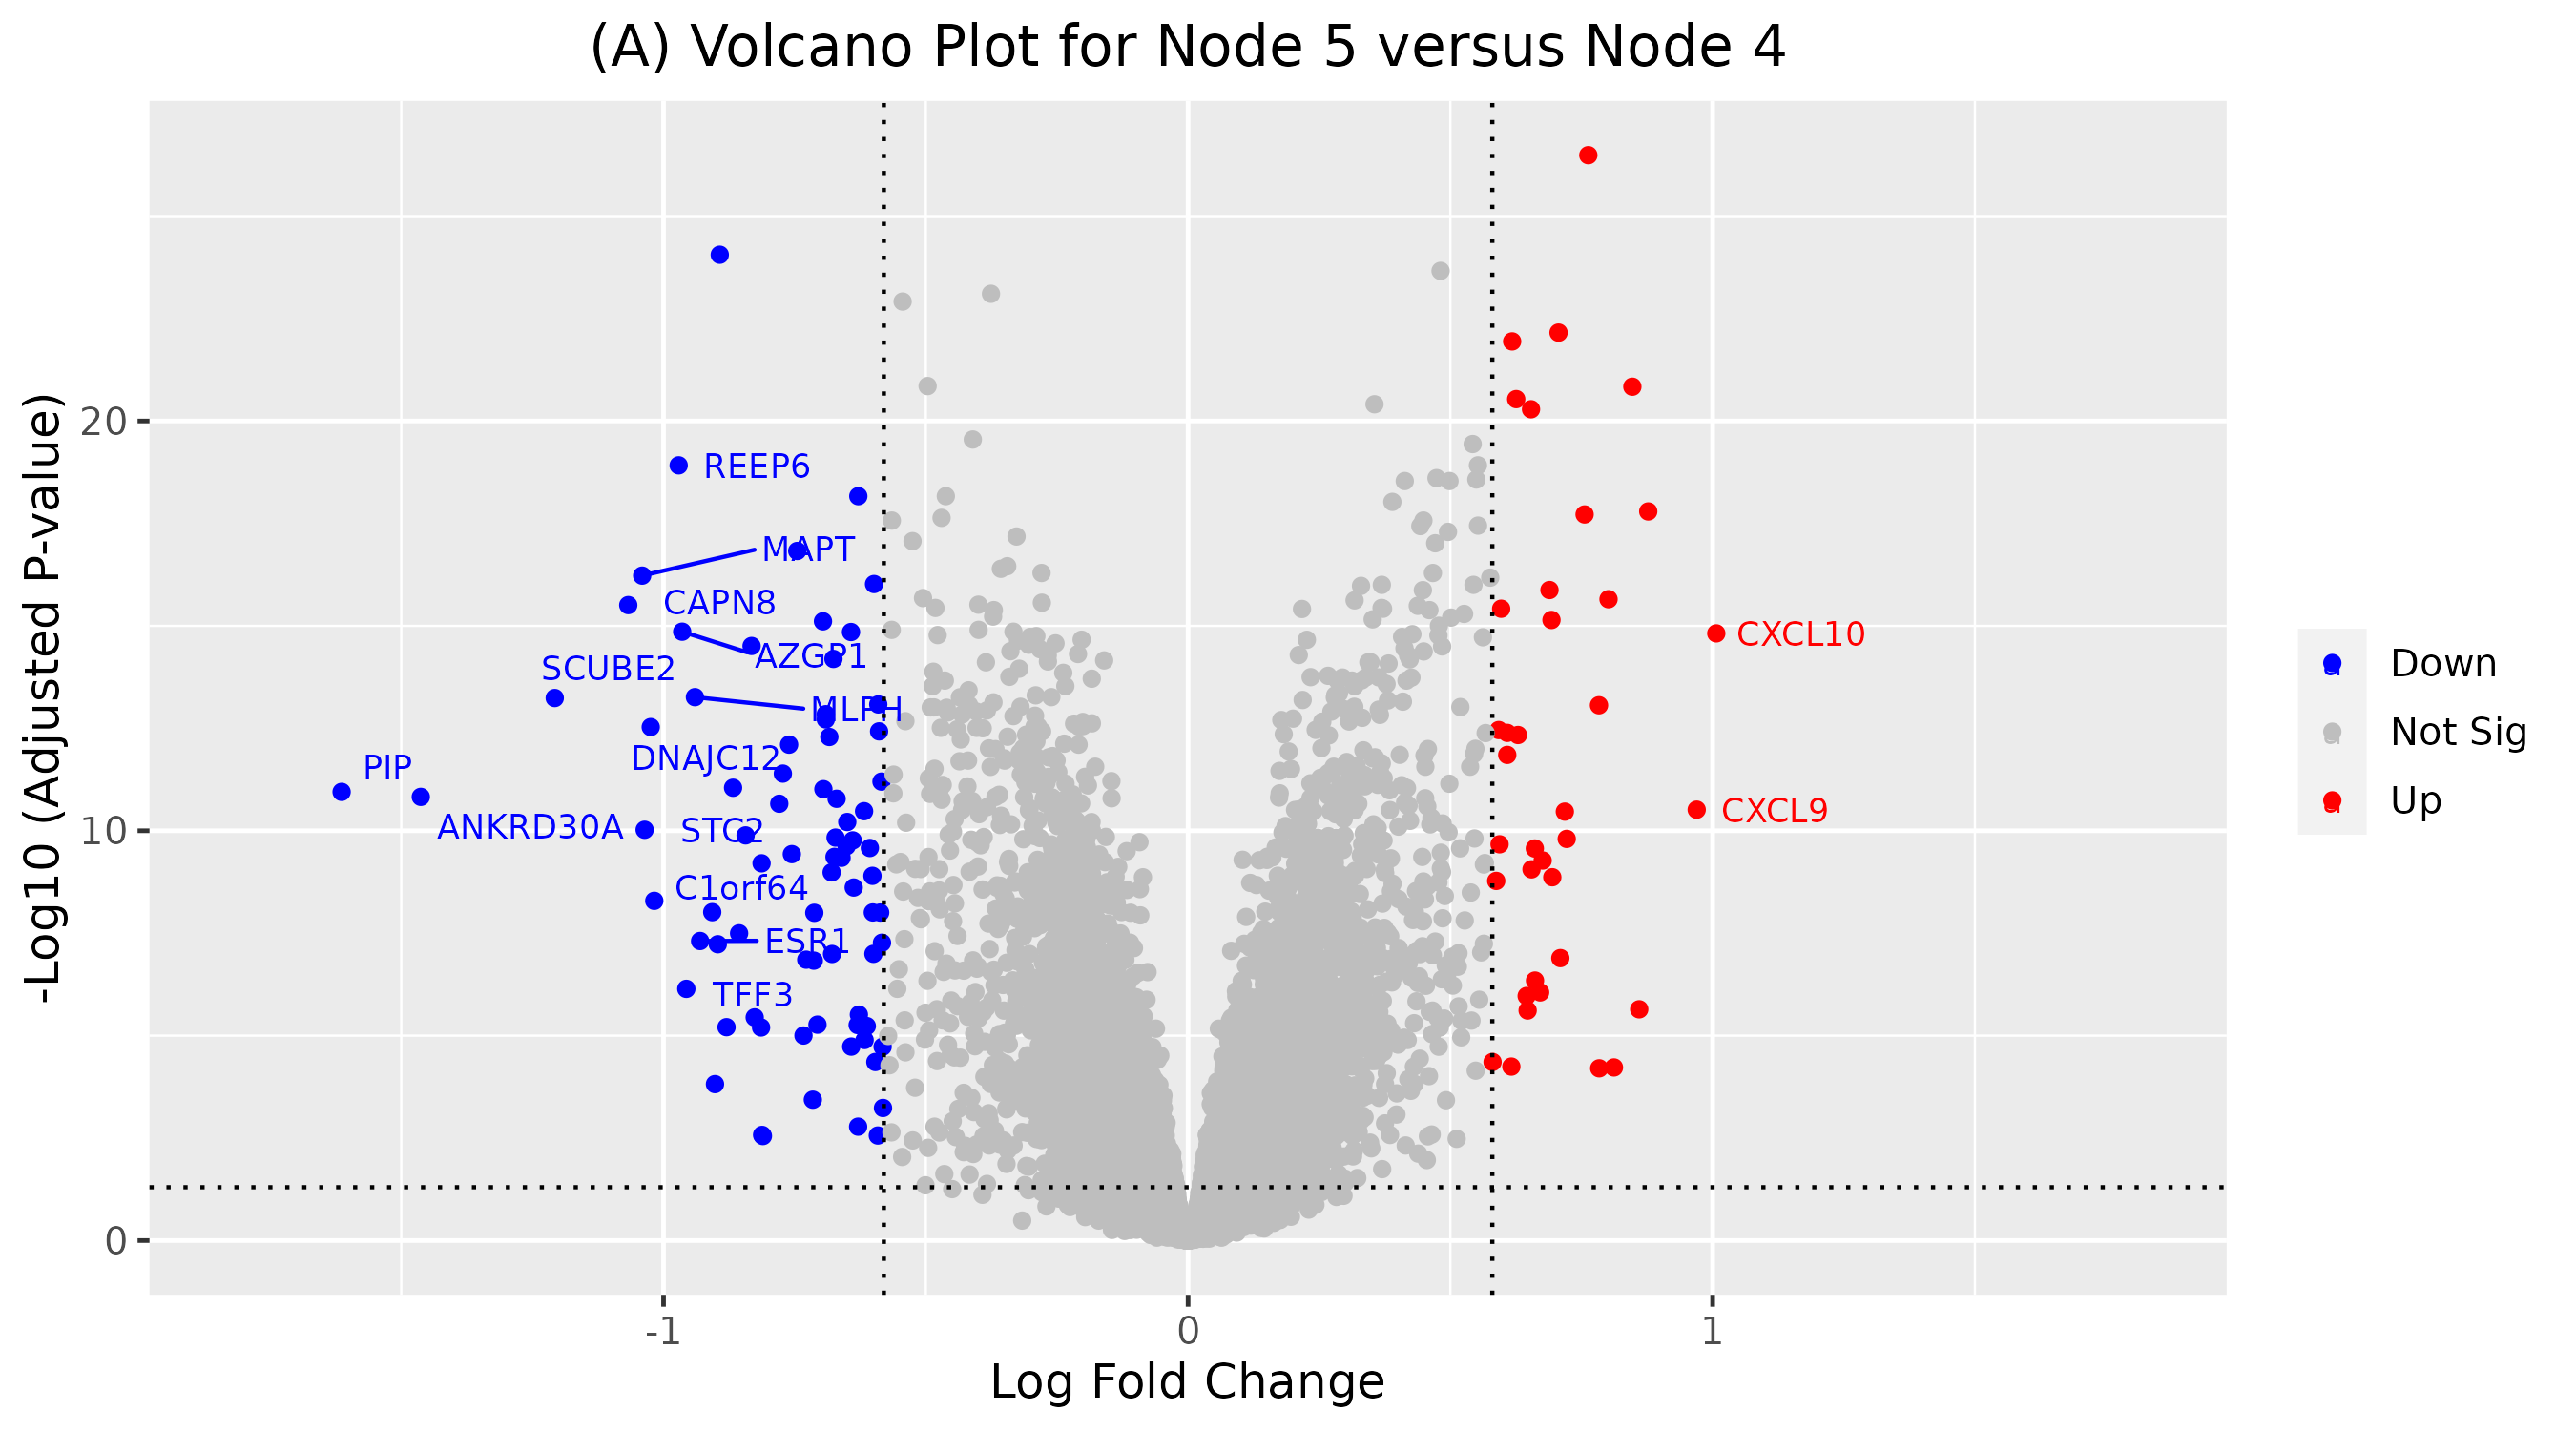
\includegraphics[width=1\linewidth]{../figures/Chapter_4/Volcano_1.png}\par 
    
\end{multicols}
\begin{multicols}{2}    
	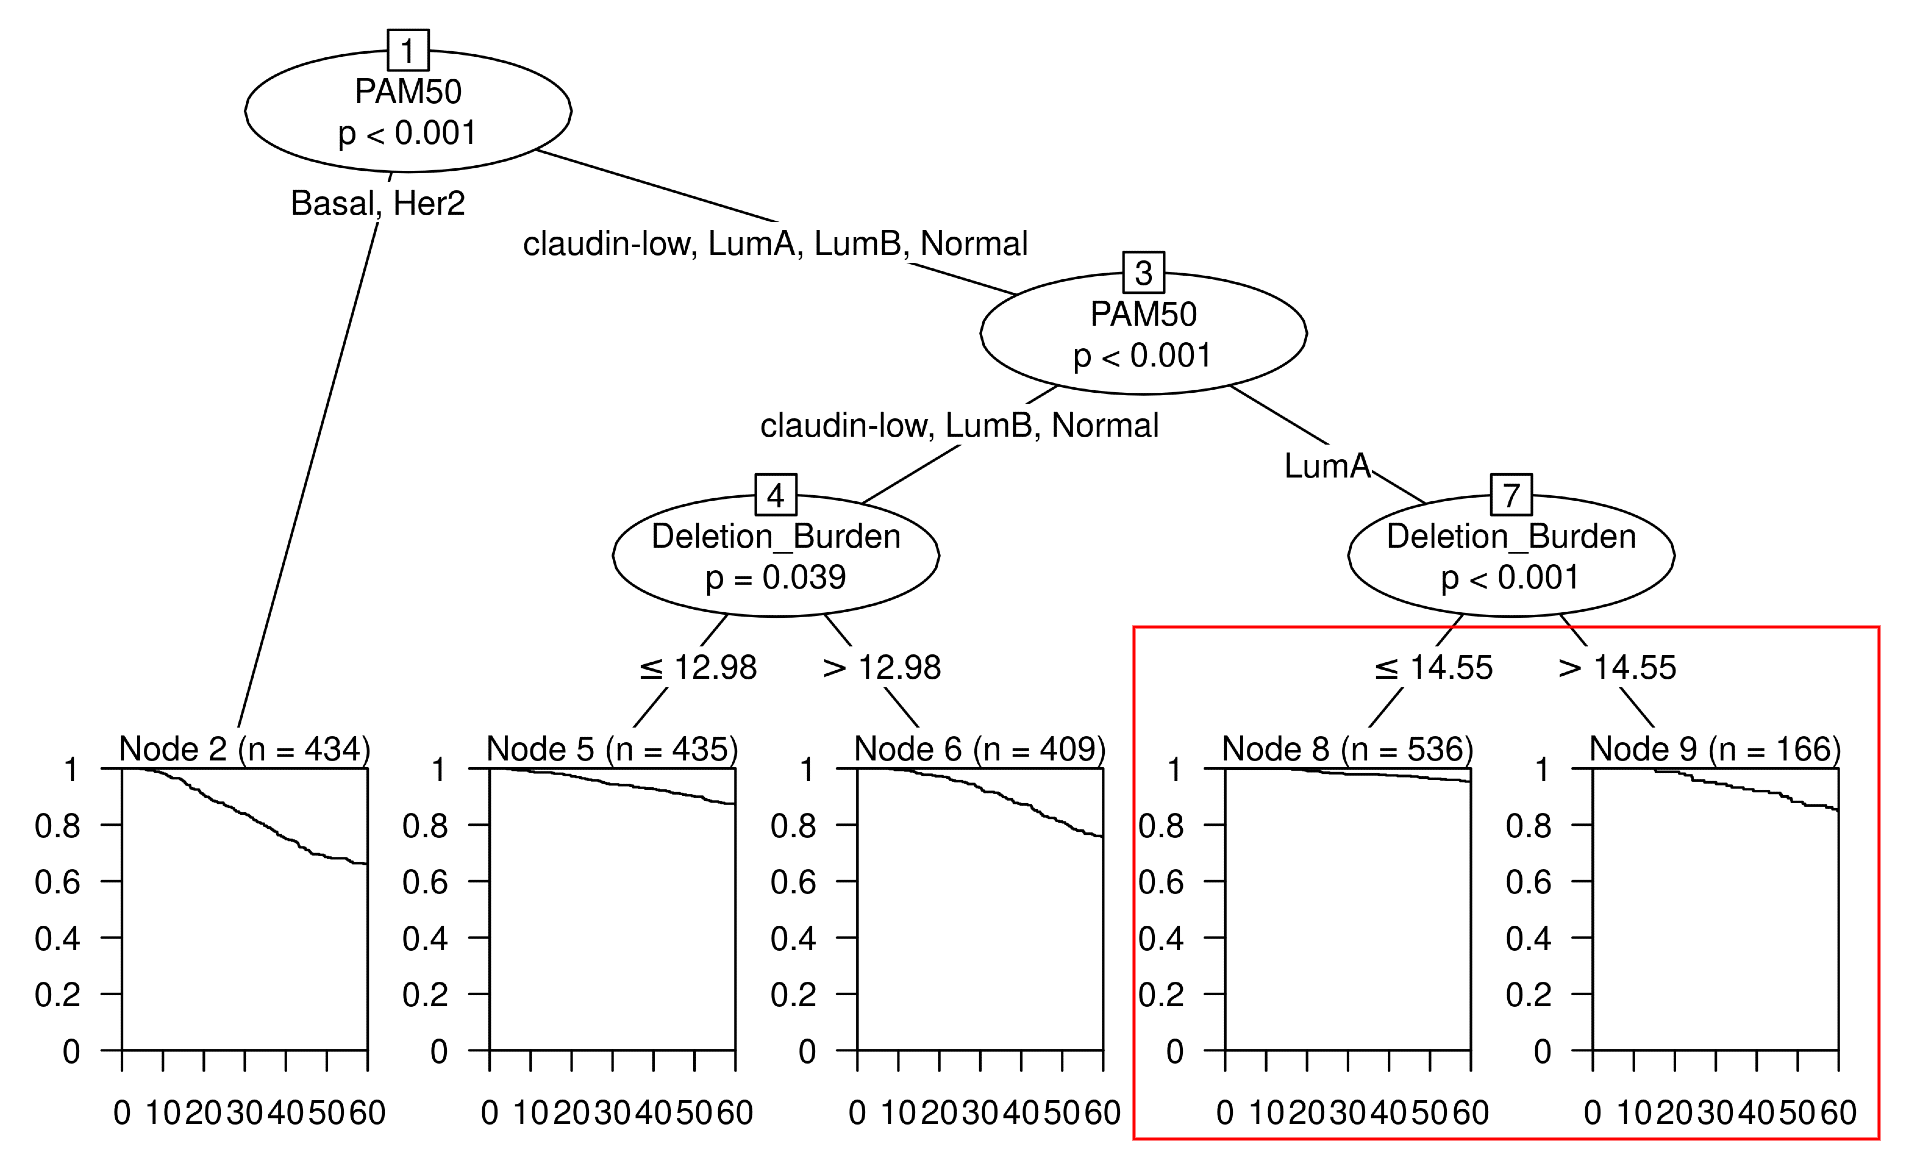
\includegraphics[width=1\linewidth]{../figures/Chapter_4/Ctree_Survival_Burden_FiveYearDSS_PAM50_Ann.png}\par 
    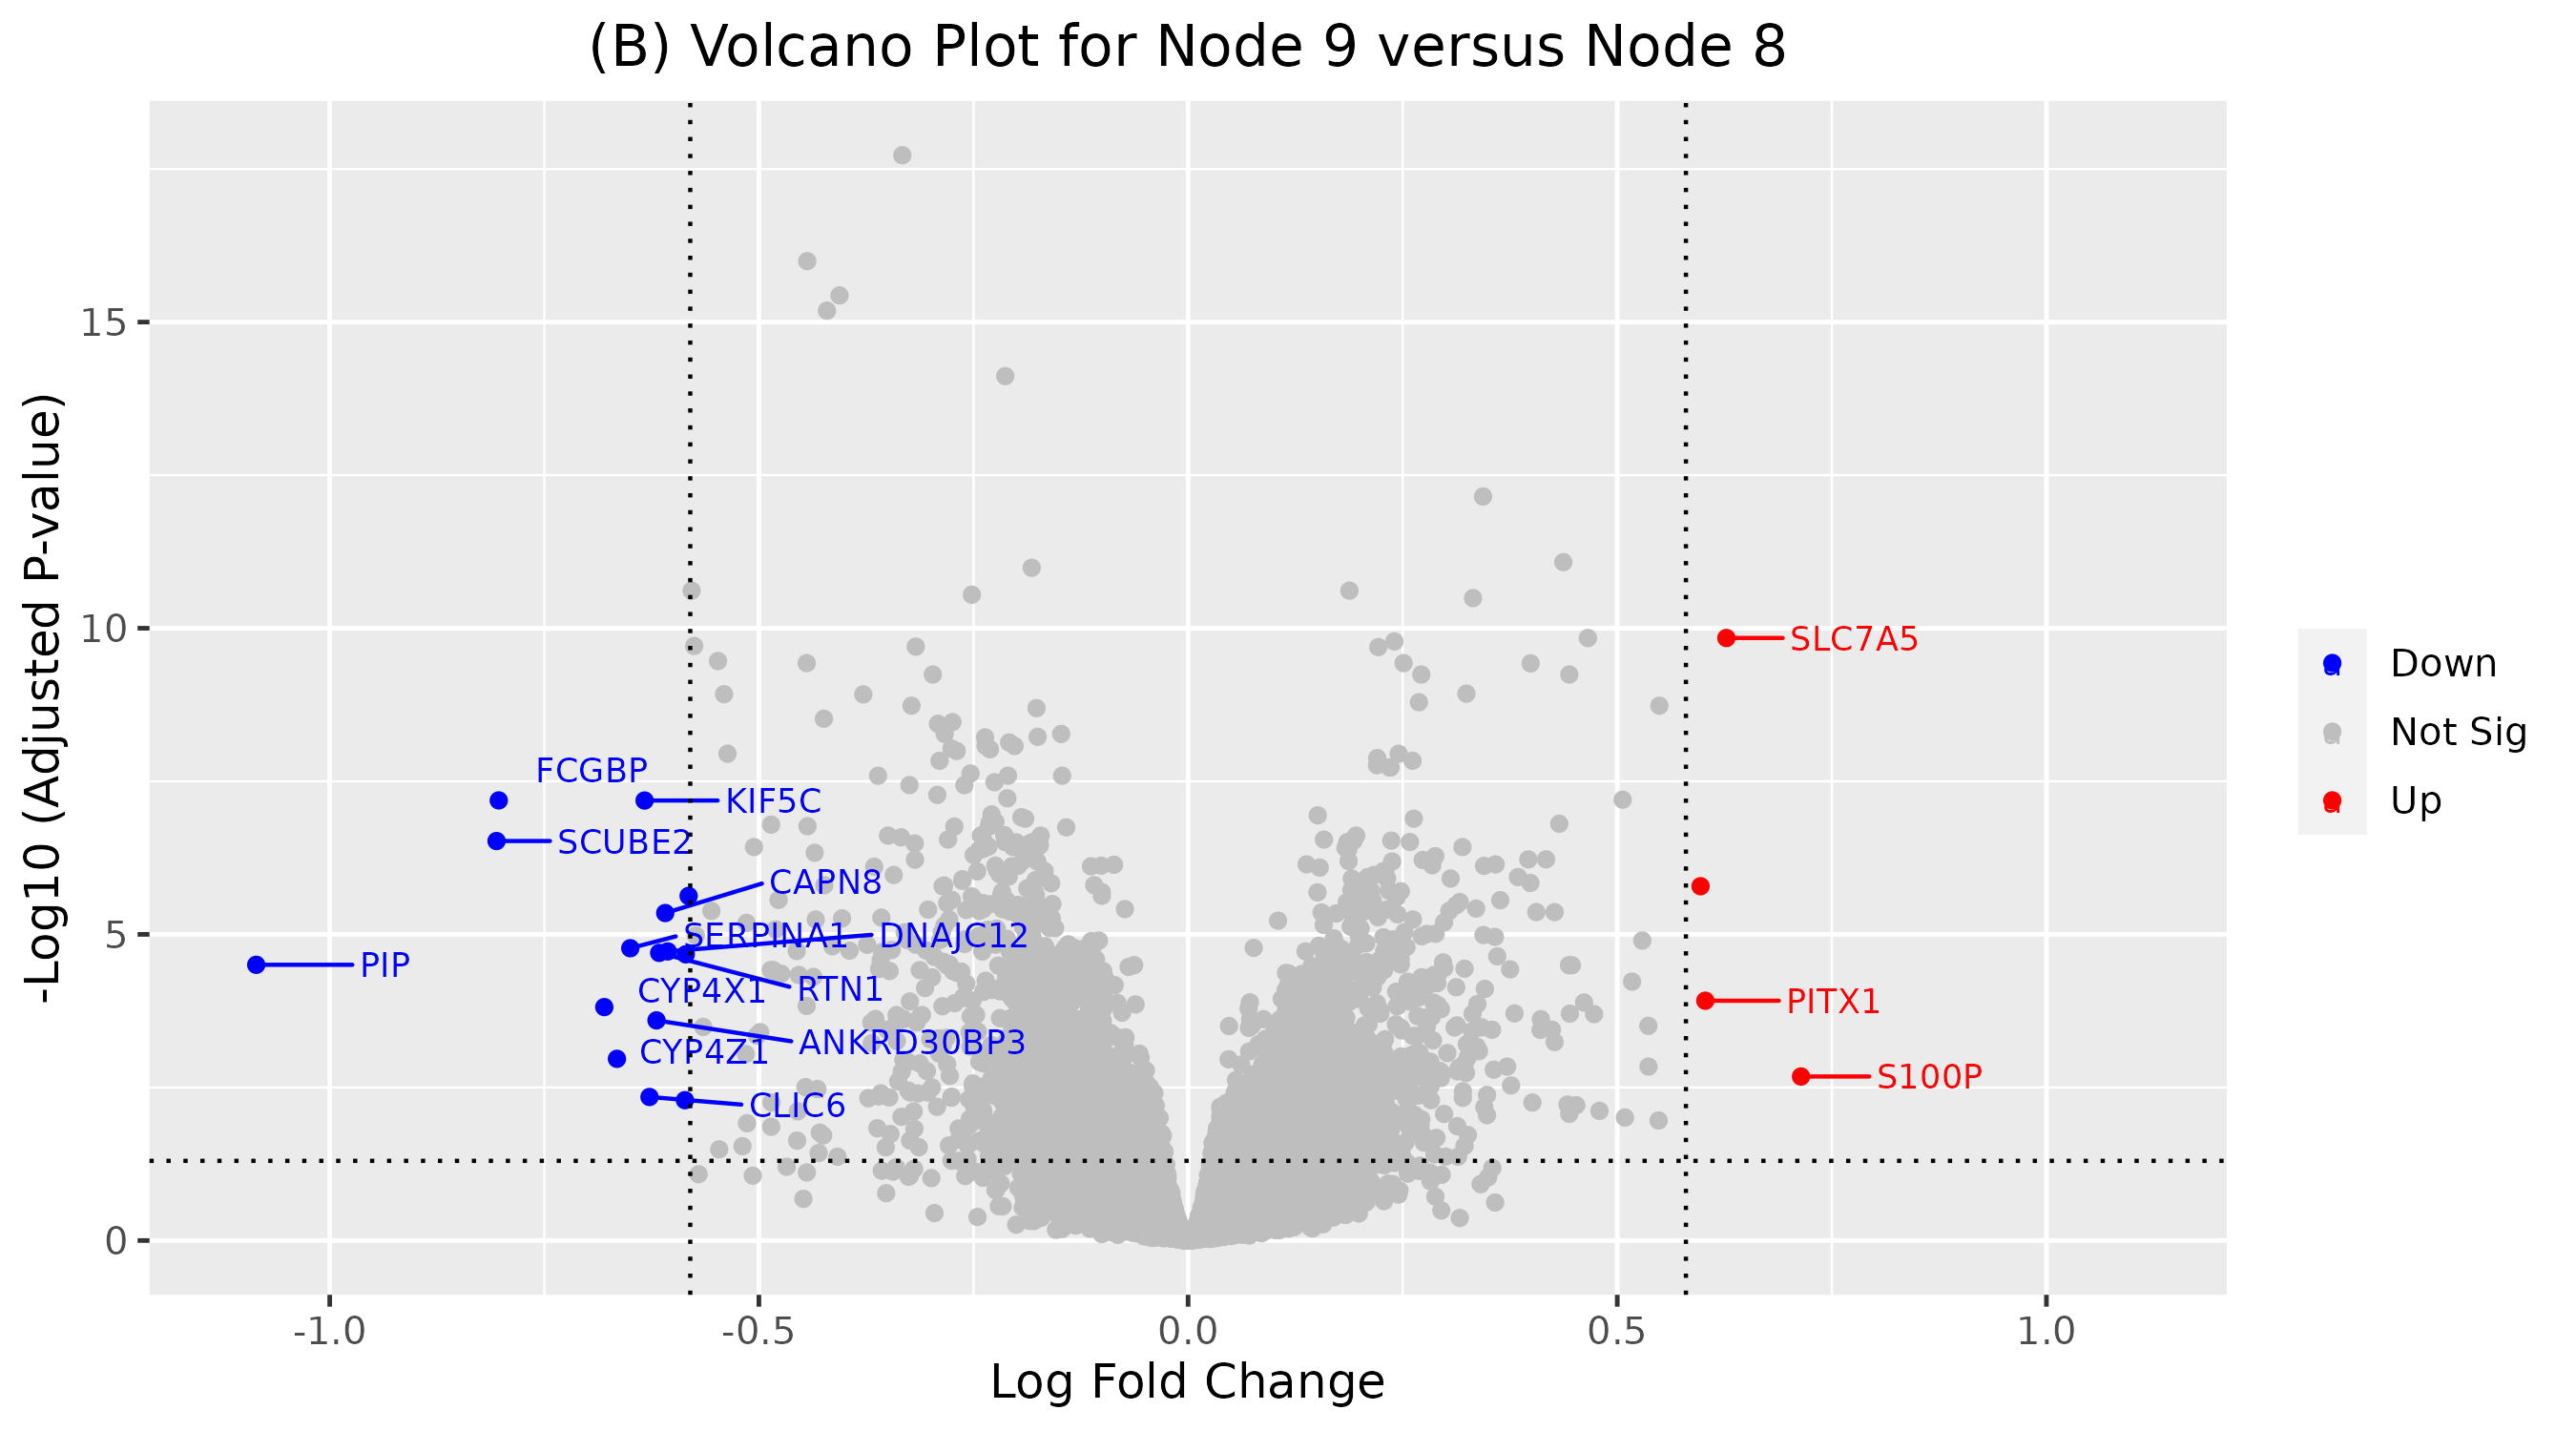
\includegraphics[width=1\linewidth]{../figures/Chapter_4/Volcano_2.png}\par 

\end{multicols}
\caption[Volcano plots resulting from DGEA applied to compare nodes informed by global CNA Burden metrics and PAM50 subtype.]{Volcano plots resulting from DGEA applied to compare nodes informed by global CNA Burden metrics and PAM50 subtype. Plots show differentially expressed genes between (A) Node 4 and Node 5 of the ctree DSS survival tree and (B) Node 8 and Node 9 of the ctree 5-year DSS survival tree.}
\label{fig:DGEA_Global_VP_PAM50}
\end{center}
\end{figure}
\vfill 

\begin{figure}[!ht]
\begin{center}
\begin{multicols}{2}
    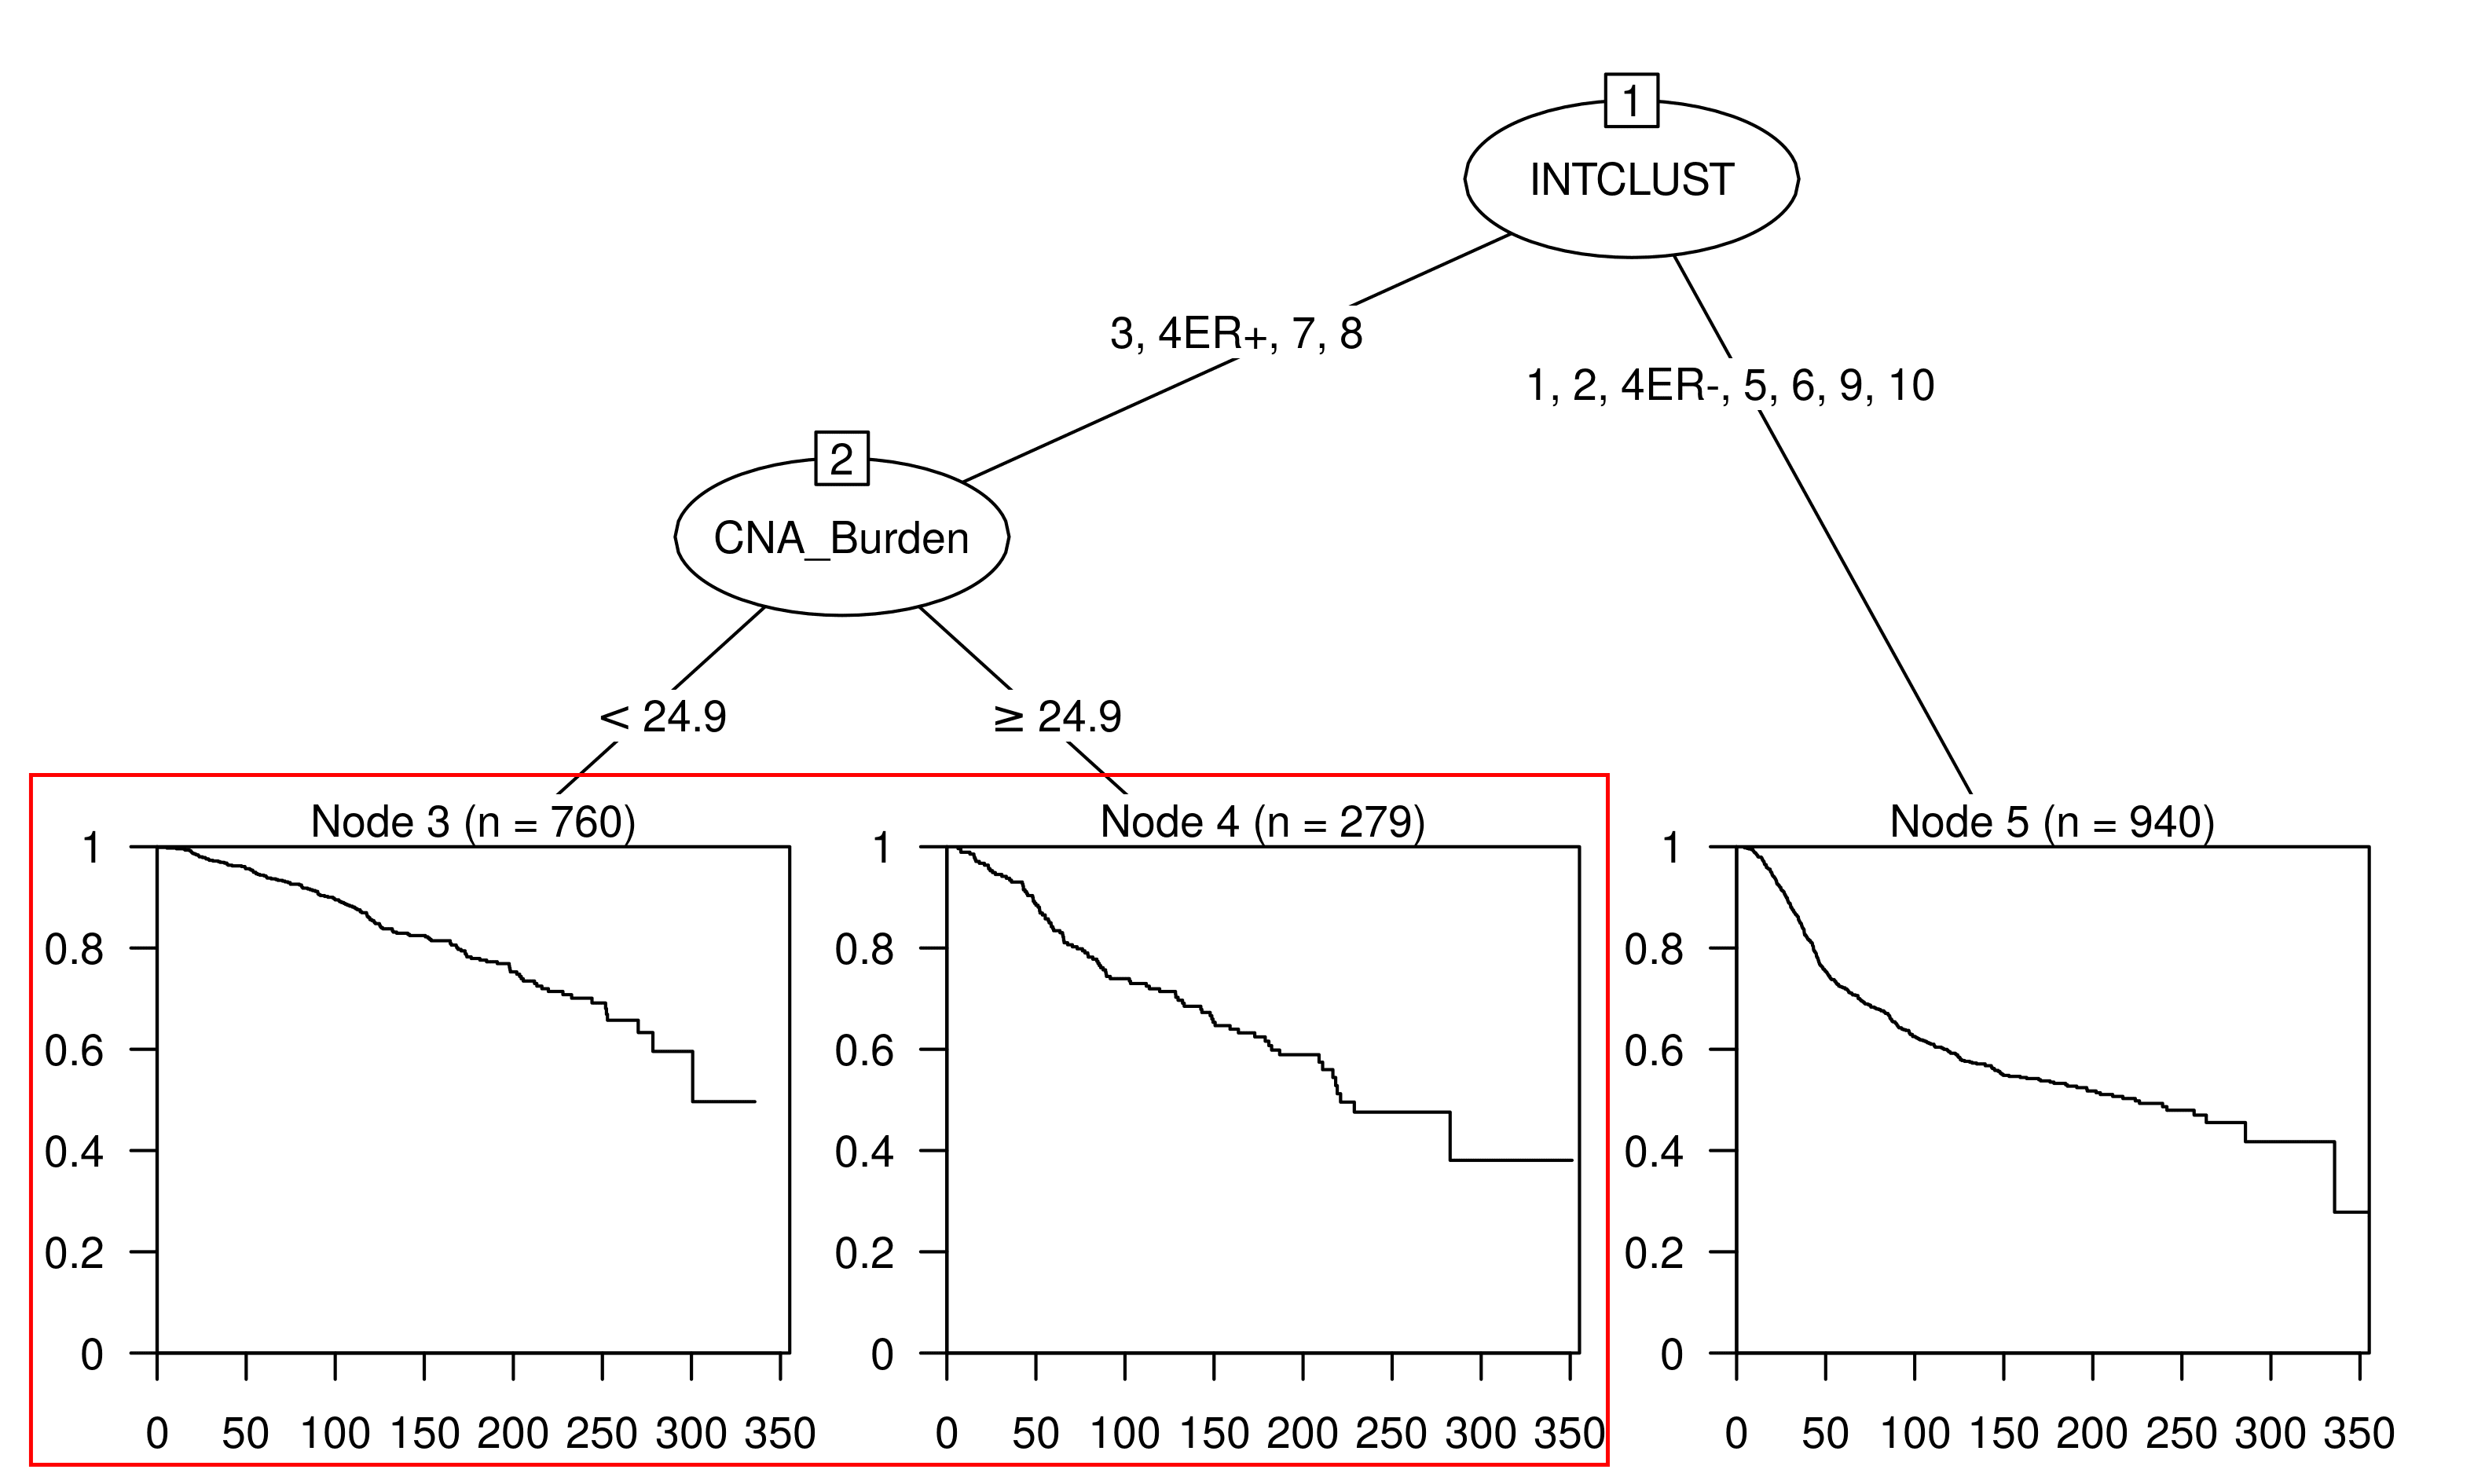
\includegraphics[width=1\linewidth]{../figures/Chapter_4/Partykit_Survival_Burden_DSS_INTCLUST_Ann.png}\par 
    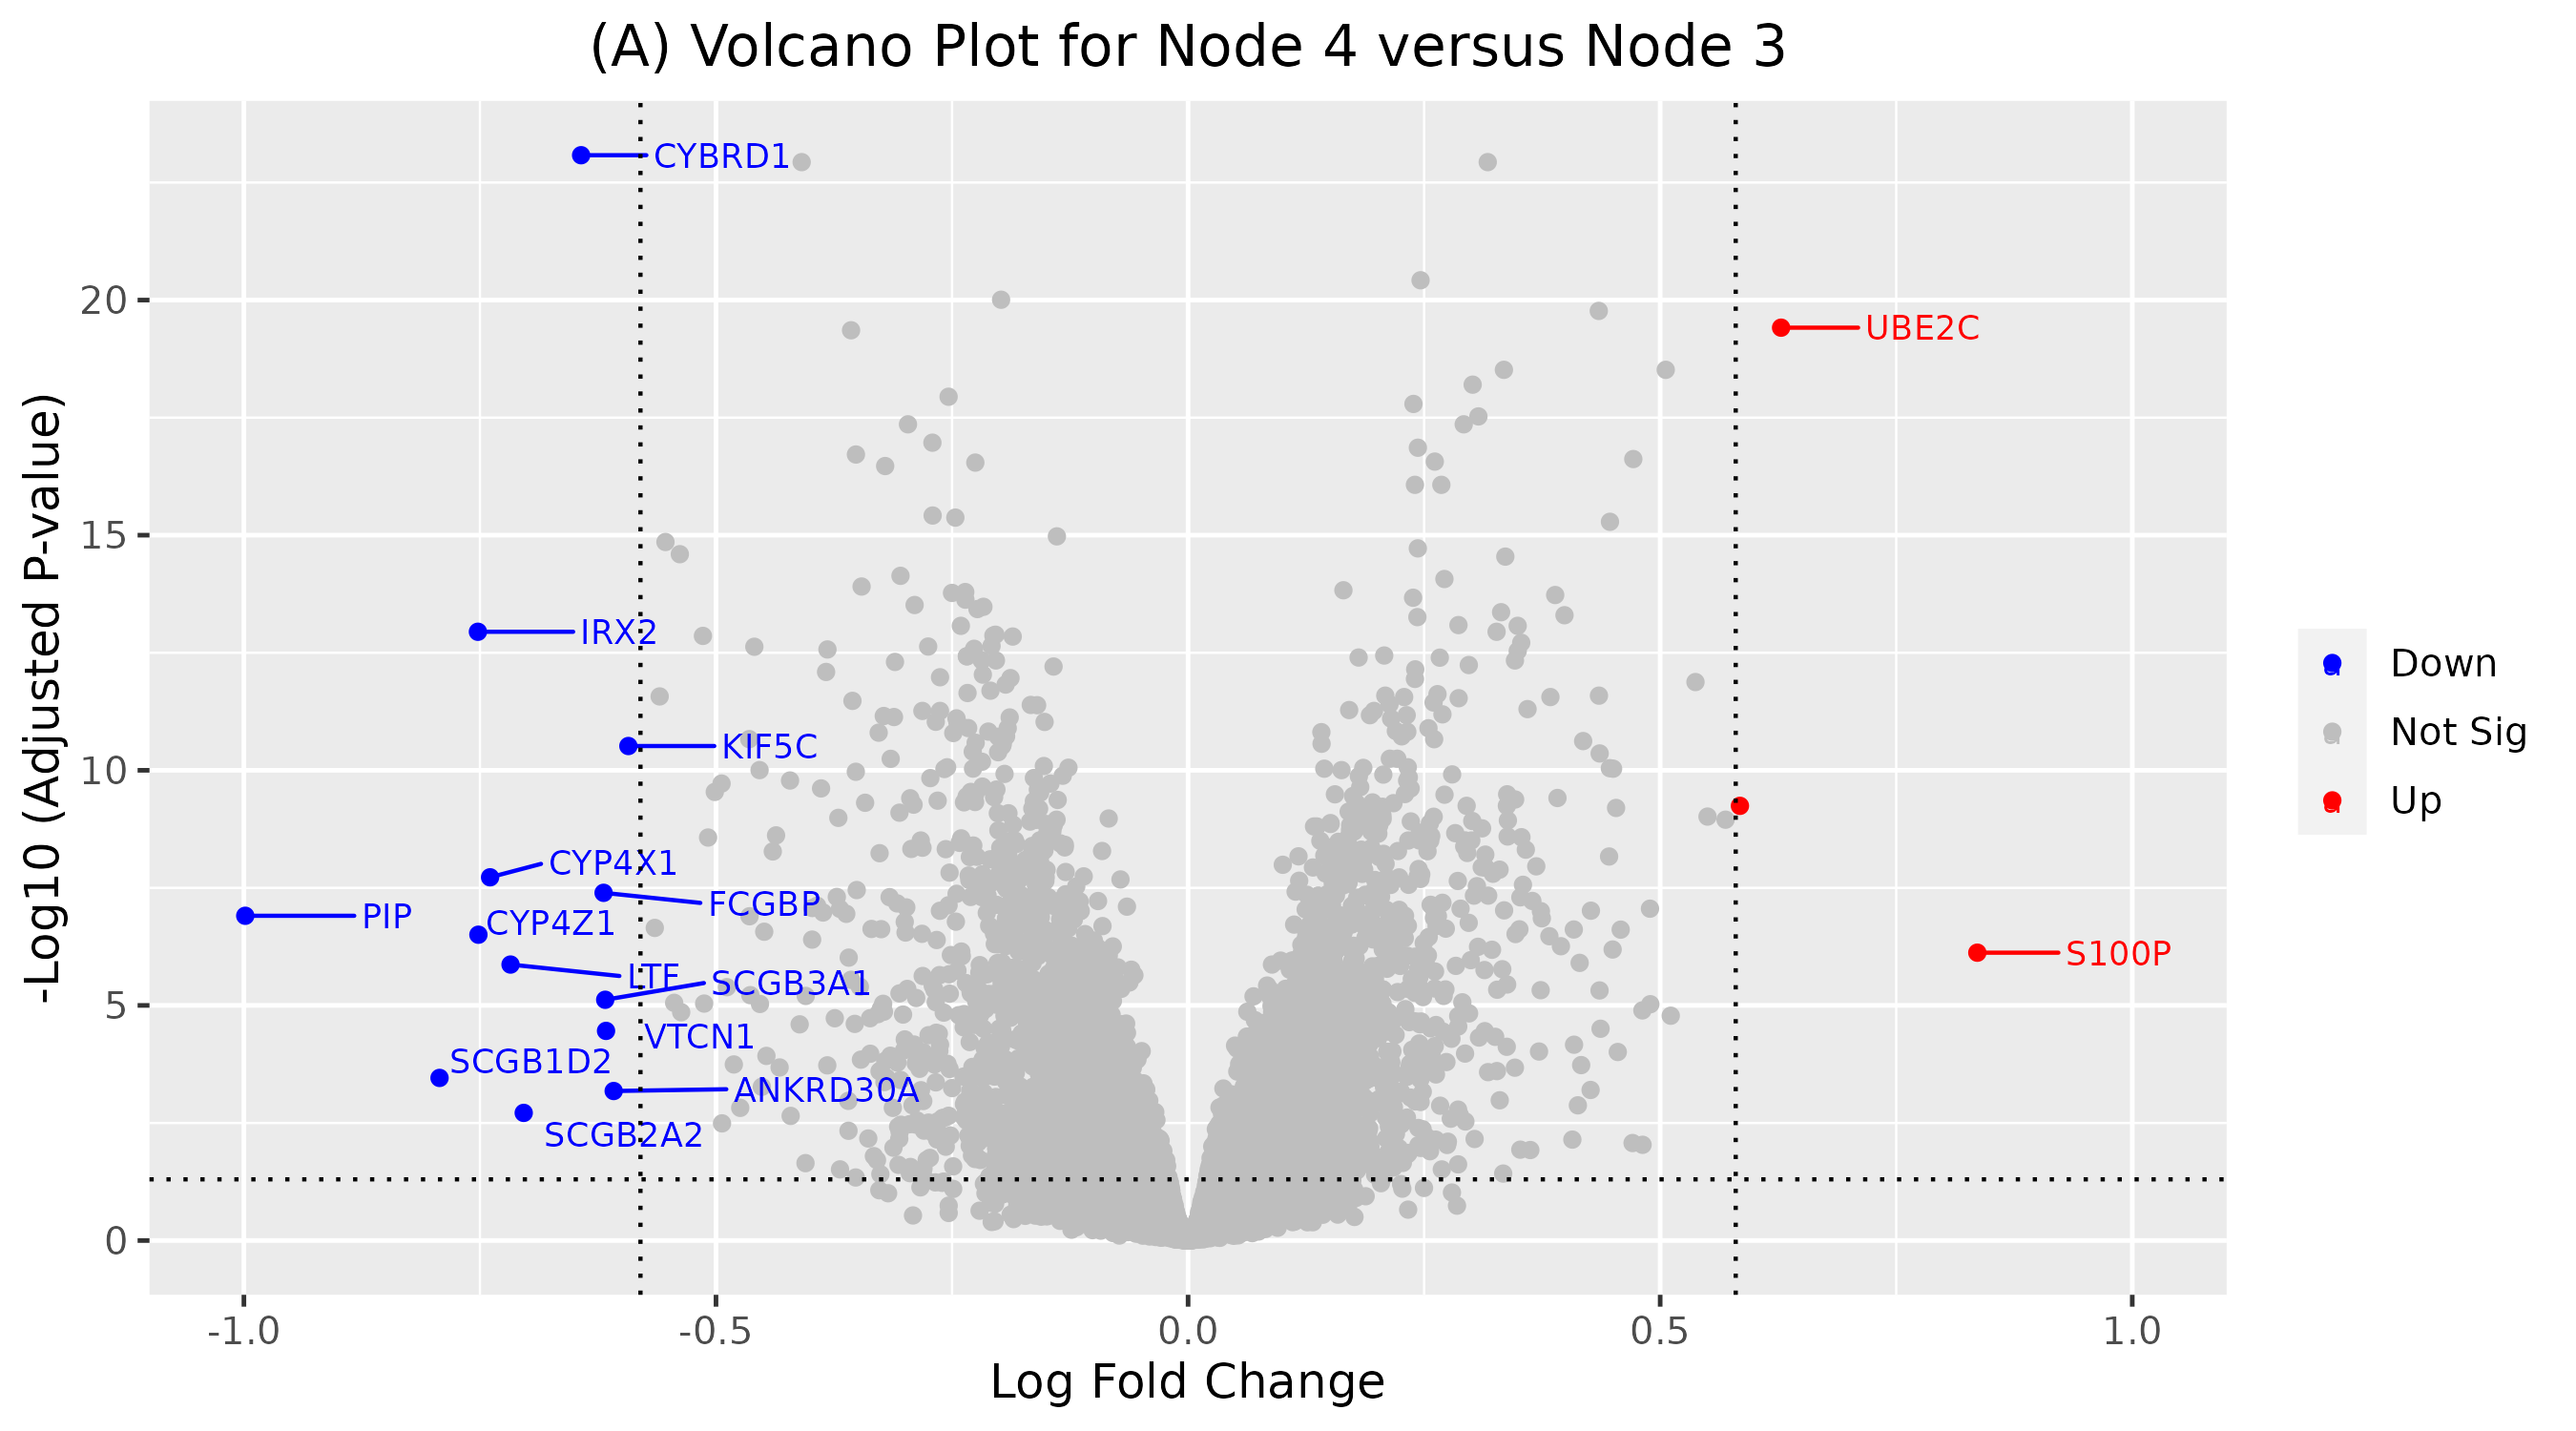
\includegraphics[width=1\linewidth]{../figures/Chapter_4/Volcano_3.png}\par 
\end{multicols}
\begin{multicols}{2}    
	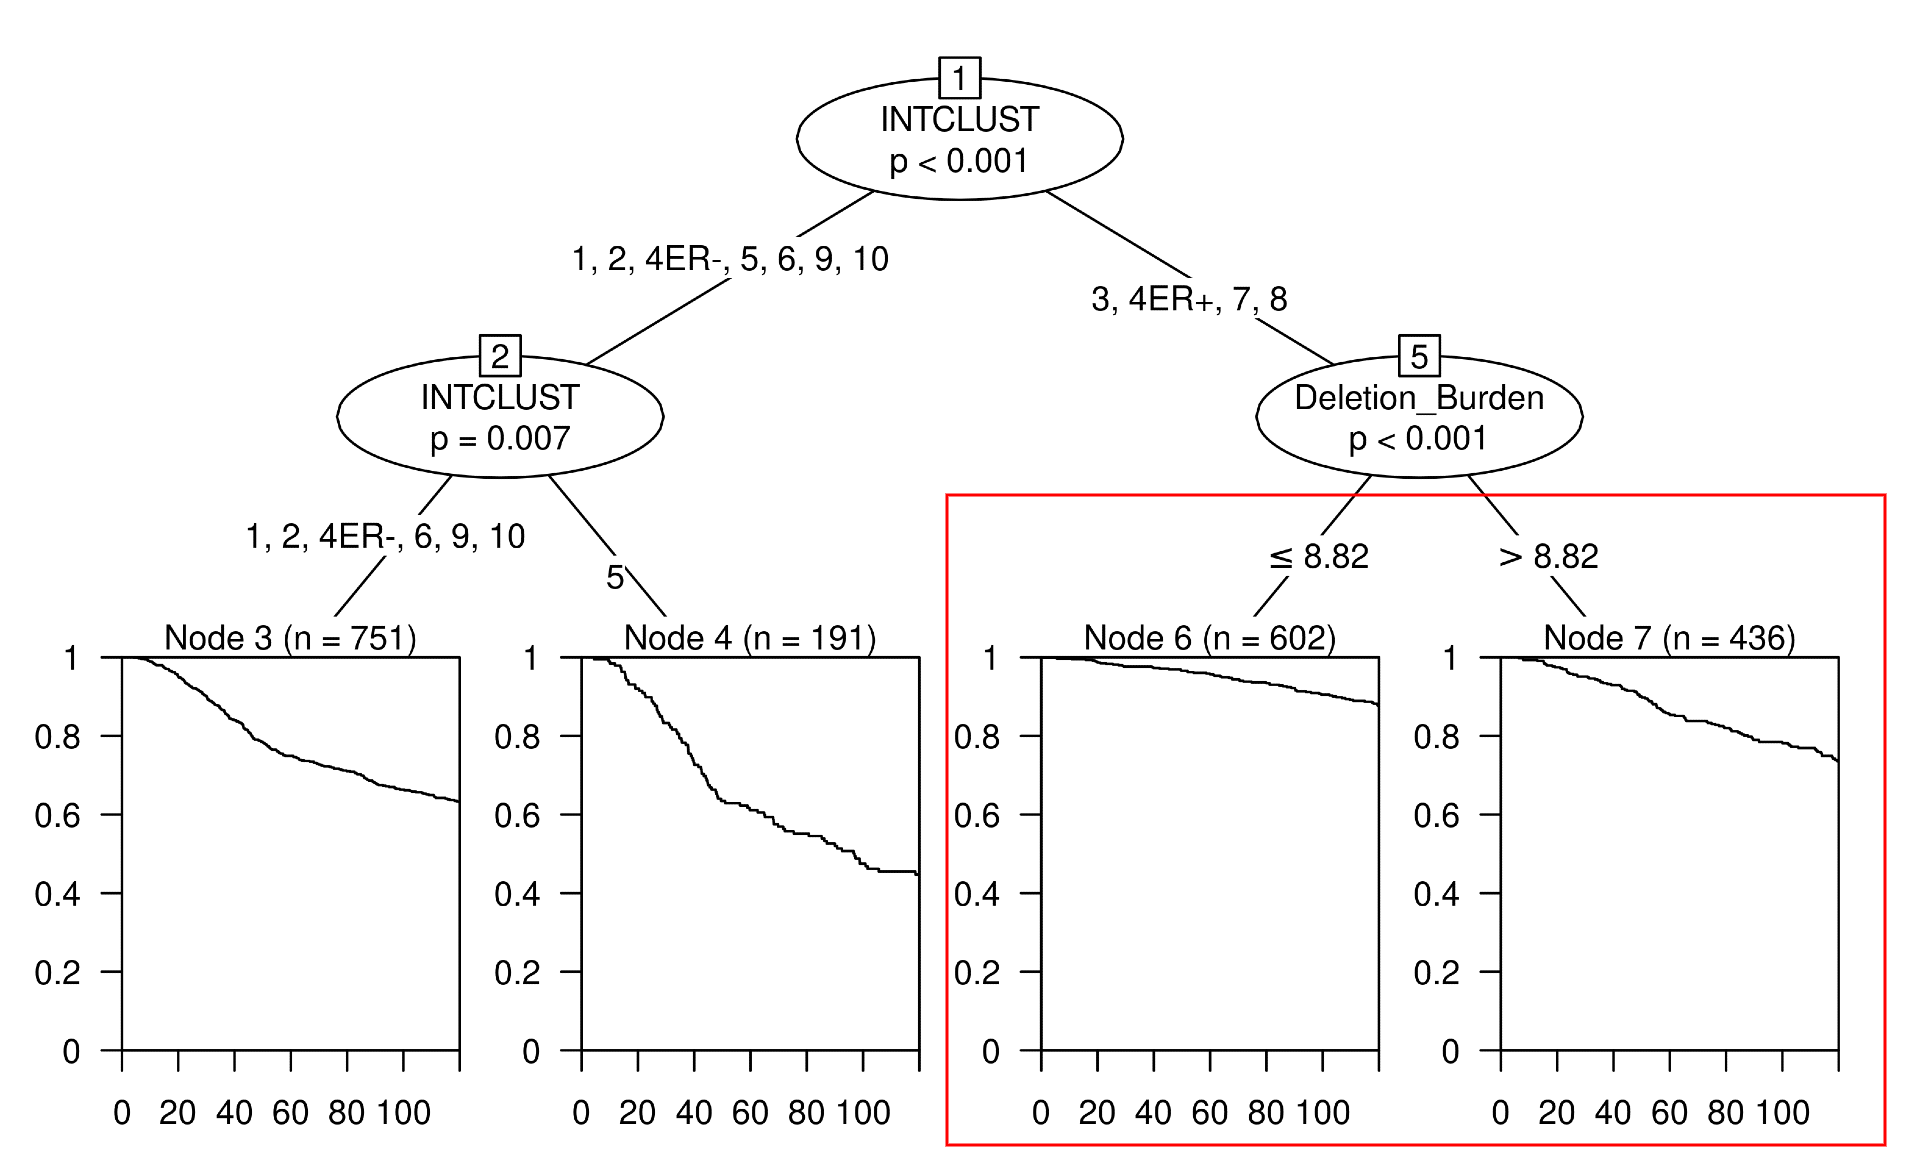
\includegraphics[width=1\linewidth]{../figures/Chapter_4/Ctree_Survival_Burden_TenYearDSS_INTCLUST_Ann.png}\par
    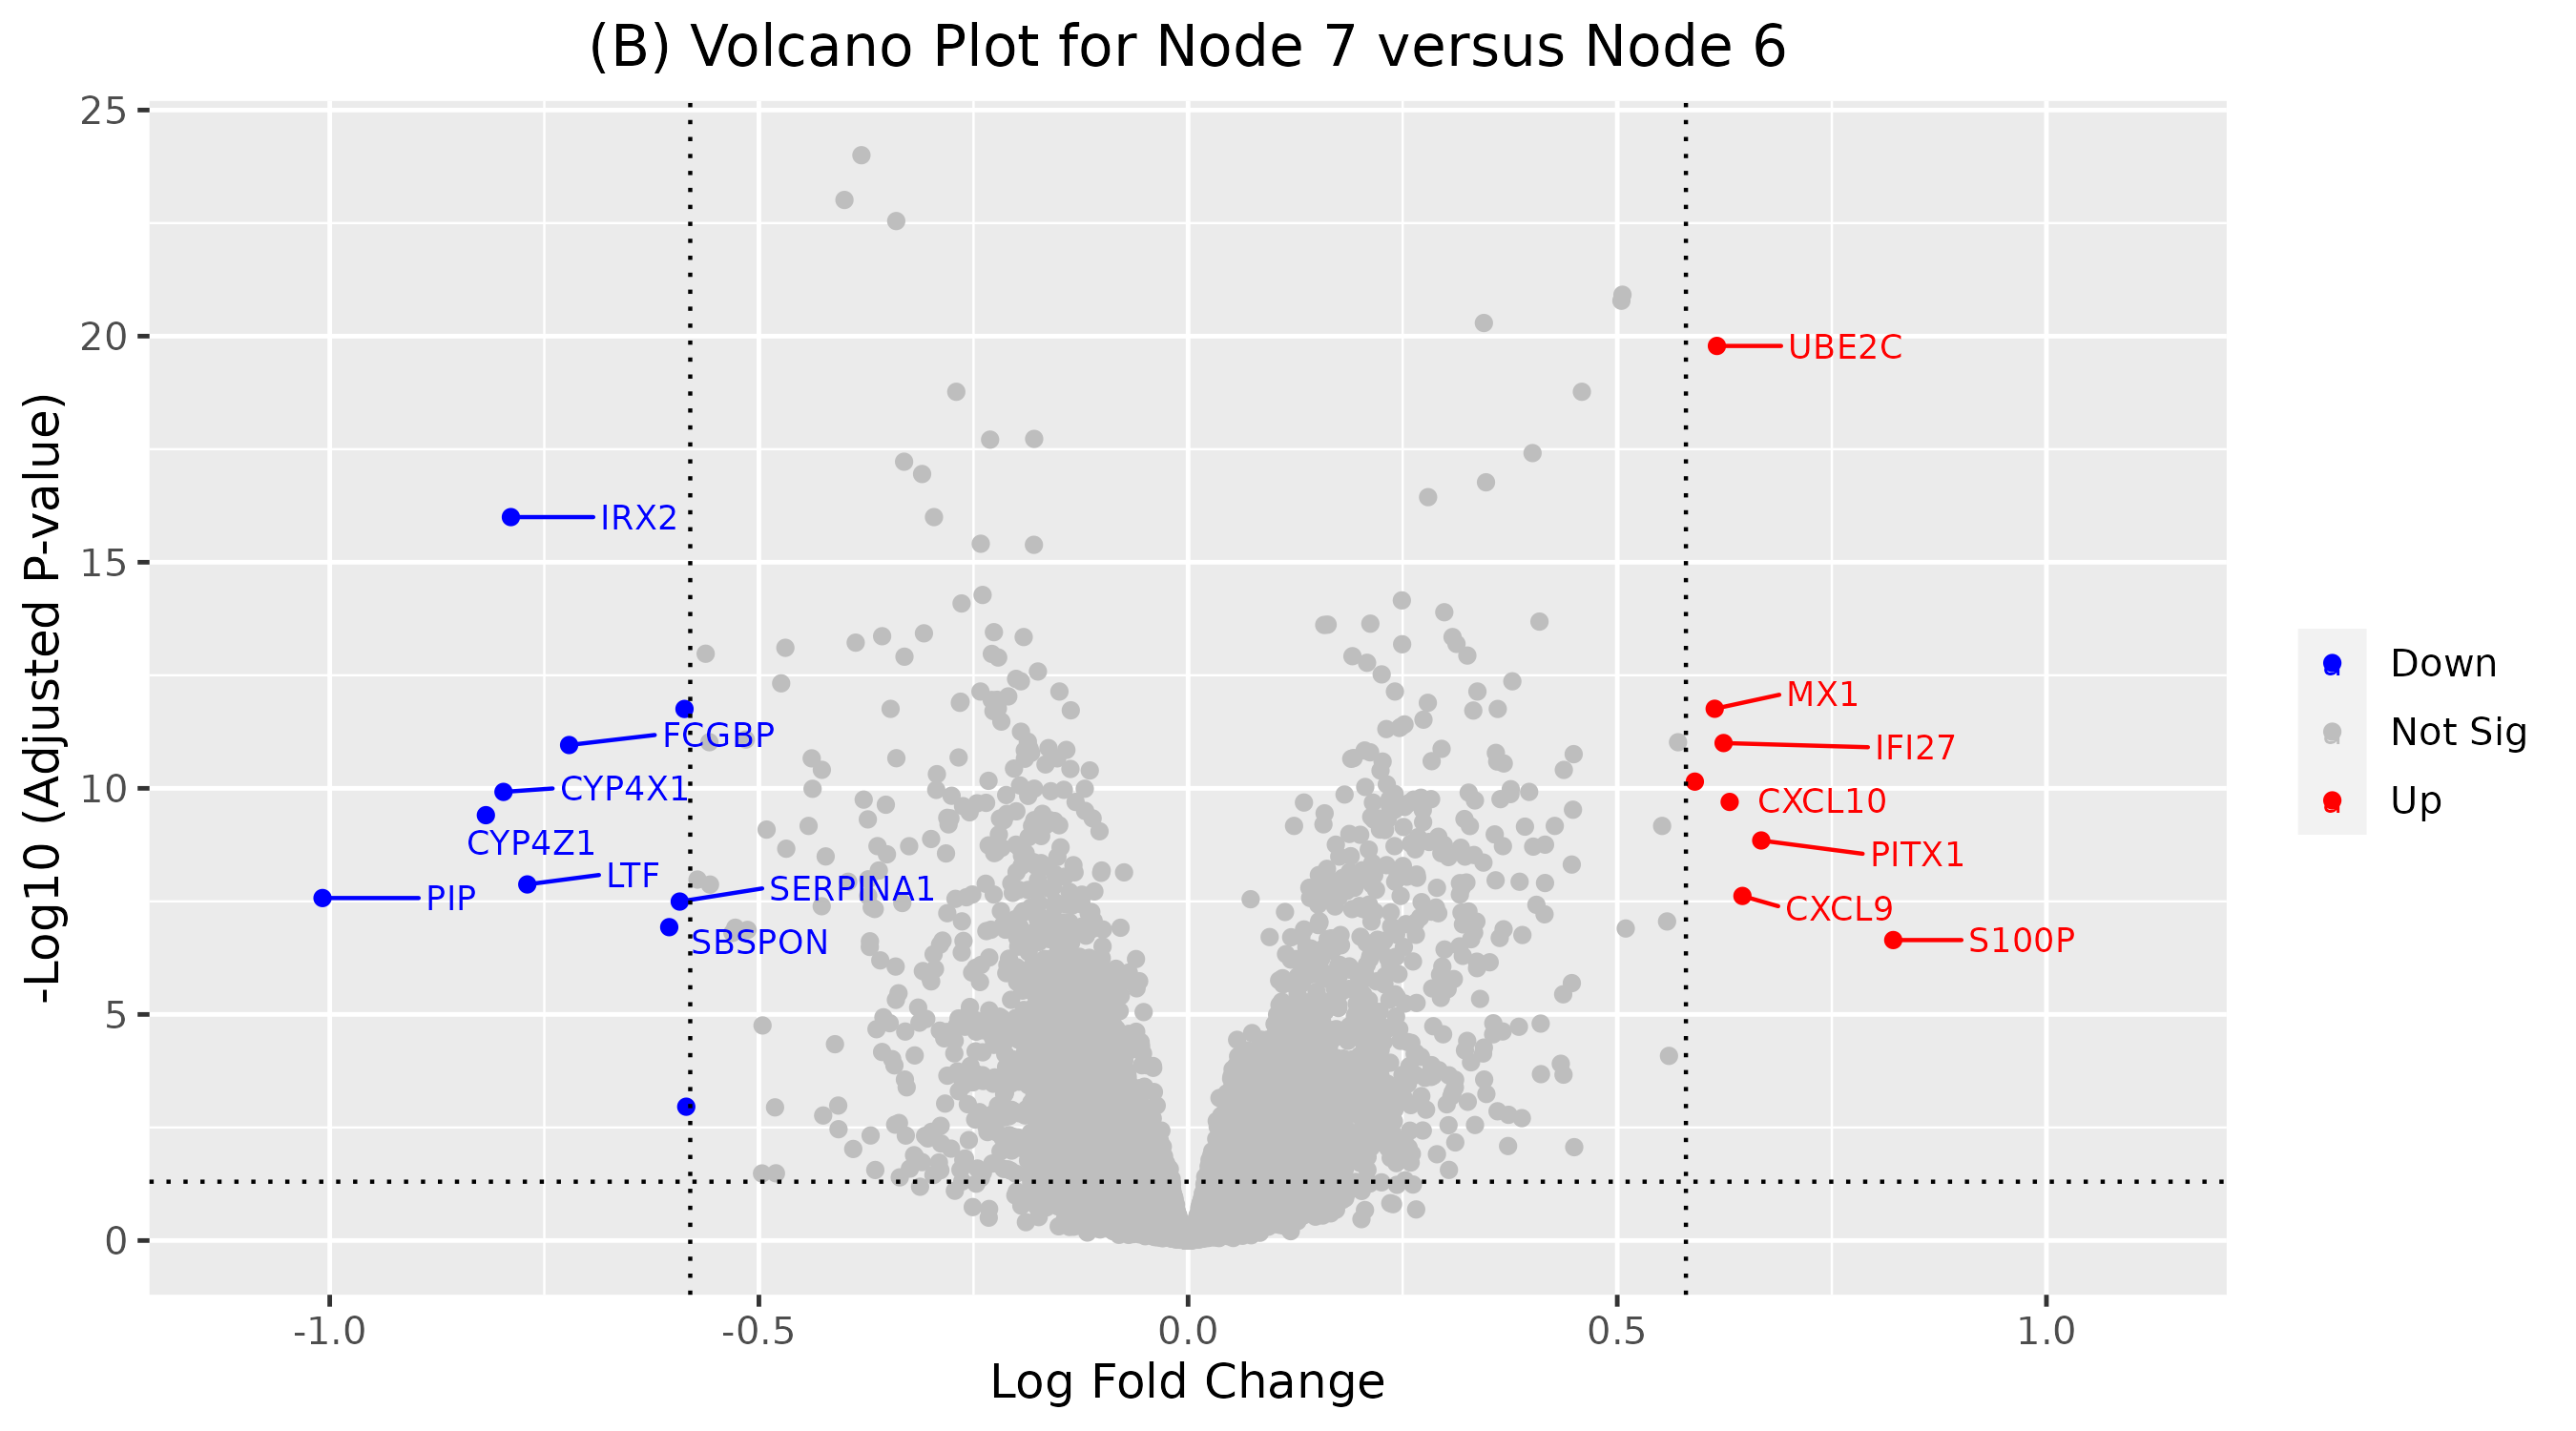
\includegraphics[width=1\linewidth]{../figures/Chapter_4/Volcano_4.png}\par 
 
\end{multicols}
\caption[Volcano plots resulting from DGEA applied to compare nodes informed by global CNA Burden metrics and IntClust.]{Volcano plots resulting from DGEA applied to compare nodes informed by global CNA Burden metrics and IntClust. Plots show differentially expressed genes between (A) Node 3 and Node 4 of the rpart DSS survival tree and (B) Node 6 and Node 7 of the ctree 10-year DSS survival tree.}
\label{fig:DGEA_Global_VP_IC}
\end{center}
\end{figure}

\subsubsection{Differential Gene Expression Analysis of Chromosome Arm CNA Metric Survival Tree Nodes}
\label{Sec_limma_2}
Section \ref{Trees_Arm} provided survival trees where splits into stratified groups of patients were informed by chromosome arm CNA burden metrics. DGEA is applied to three survival trees of particular interest. The DSS ctree survival tree utilising the PAM50 subtype molecular classification (Figure \ref{fig:PAM50_PA_CNA_Burden_DSS}) indicated that Luminal A and Claudin-low patients can be further stratified into two nodes: Node 4 and Node 5, classified by CNA Del Burden of chromosome 3p. Higher chromosome 3p CNA Del Burden, above an optimised threshold of 30.21\%, partitioned patients into Node 5 with poorer DSS survival profile. DGEA comparing gene expression between Node 4 (low CNA Del Burden on chromosome 3p) and Node 5 (high CNA Del Burden on chromosome 3p), indicates that the genes LZTFL1, IMPDH2, ZMYND10, LRIG1, P4HTM, FLNB, MST1, GPD1L, KCTD6, ACOX2, LTF, located on chromosome 3p, are down-regulated in Node 5 compared to Node 4 (Figure \ref{fig:Volcano_chr_total}A and B). 

The DSS rpart survival tree utilising the IntClust molecular classification (Figure \ref{fig:INTCLUST_PA_CNA_Burden_DSS}) indicated that for IntClust 3, 4ER+, 7 and 8 patients, CNA Del Burden on chromosome 18q partitions patients into Node 3, CNA Del Burden $<69.78\%$ with better DSS outcome and Node 4, CNA Del Burden $\geq 69.78\%$ with poorer DSS outcome. DGEA comparing gene expression between Node 3 (low CNA Del Burden on chromosome 18q) and Node 4 (high CNA Del Burden on chromosome 18q), indicates that 23 genes are down-regulated and 19 are up-regulated in Node 4 compared to Node 3. There is one gene located on chromosome 18q that is classified as down-regulated in patients with higher levels of deletions on chromosome 18q, BCL2. 

The 5-year DSS rpart survival tree utilsiing the PAM50 subtype molecular classification (Figure \ref{fig:PAM50_PA_CNA_Burden_FiveYearDSS}) indicated that for Luminal A patients, CNA Del Burden on chromosome 11p, above 7.72\%, is associated with poorer 5-year DSS outcome. DGEA comparing gene expression between Node 3 (low CNA Del Burden on chromosome 11p) and Node 4 (high CNA Del Burden on chromosome 11p), indicates that no genes, located on chromosome 11p, are differentially expressed in Node 4 compared to Node 3. 

Comparing the gene expression profiles of the survival tree nodes for focused examples of interest, produced using the global and chromosome arm CNA Burden metrics, indicates there is widespread differential gene expression between Node partitions. 

\vfill
\begin{figure}[H]
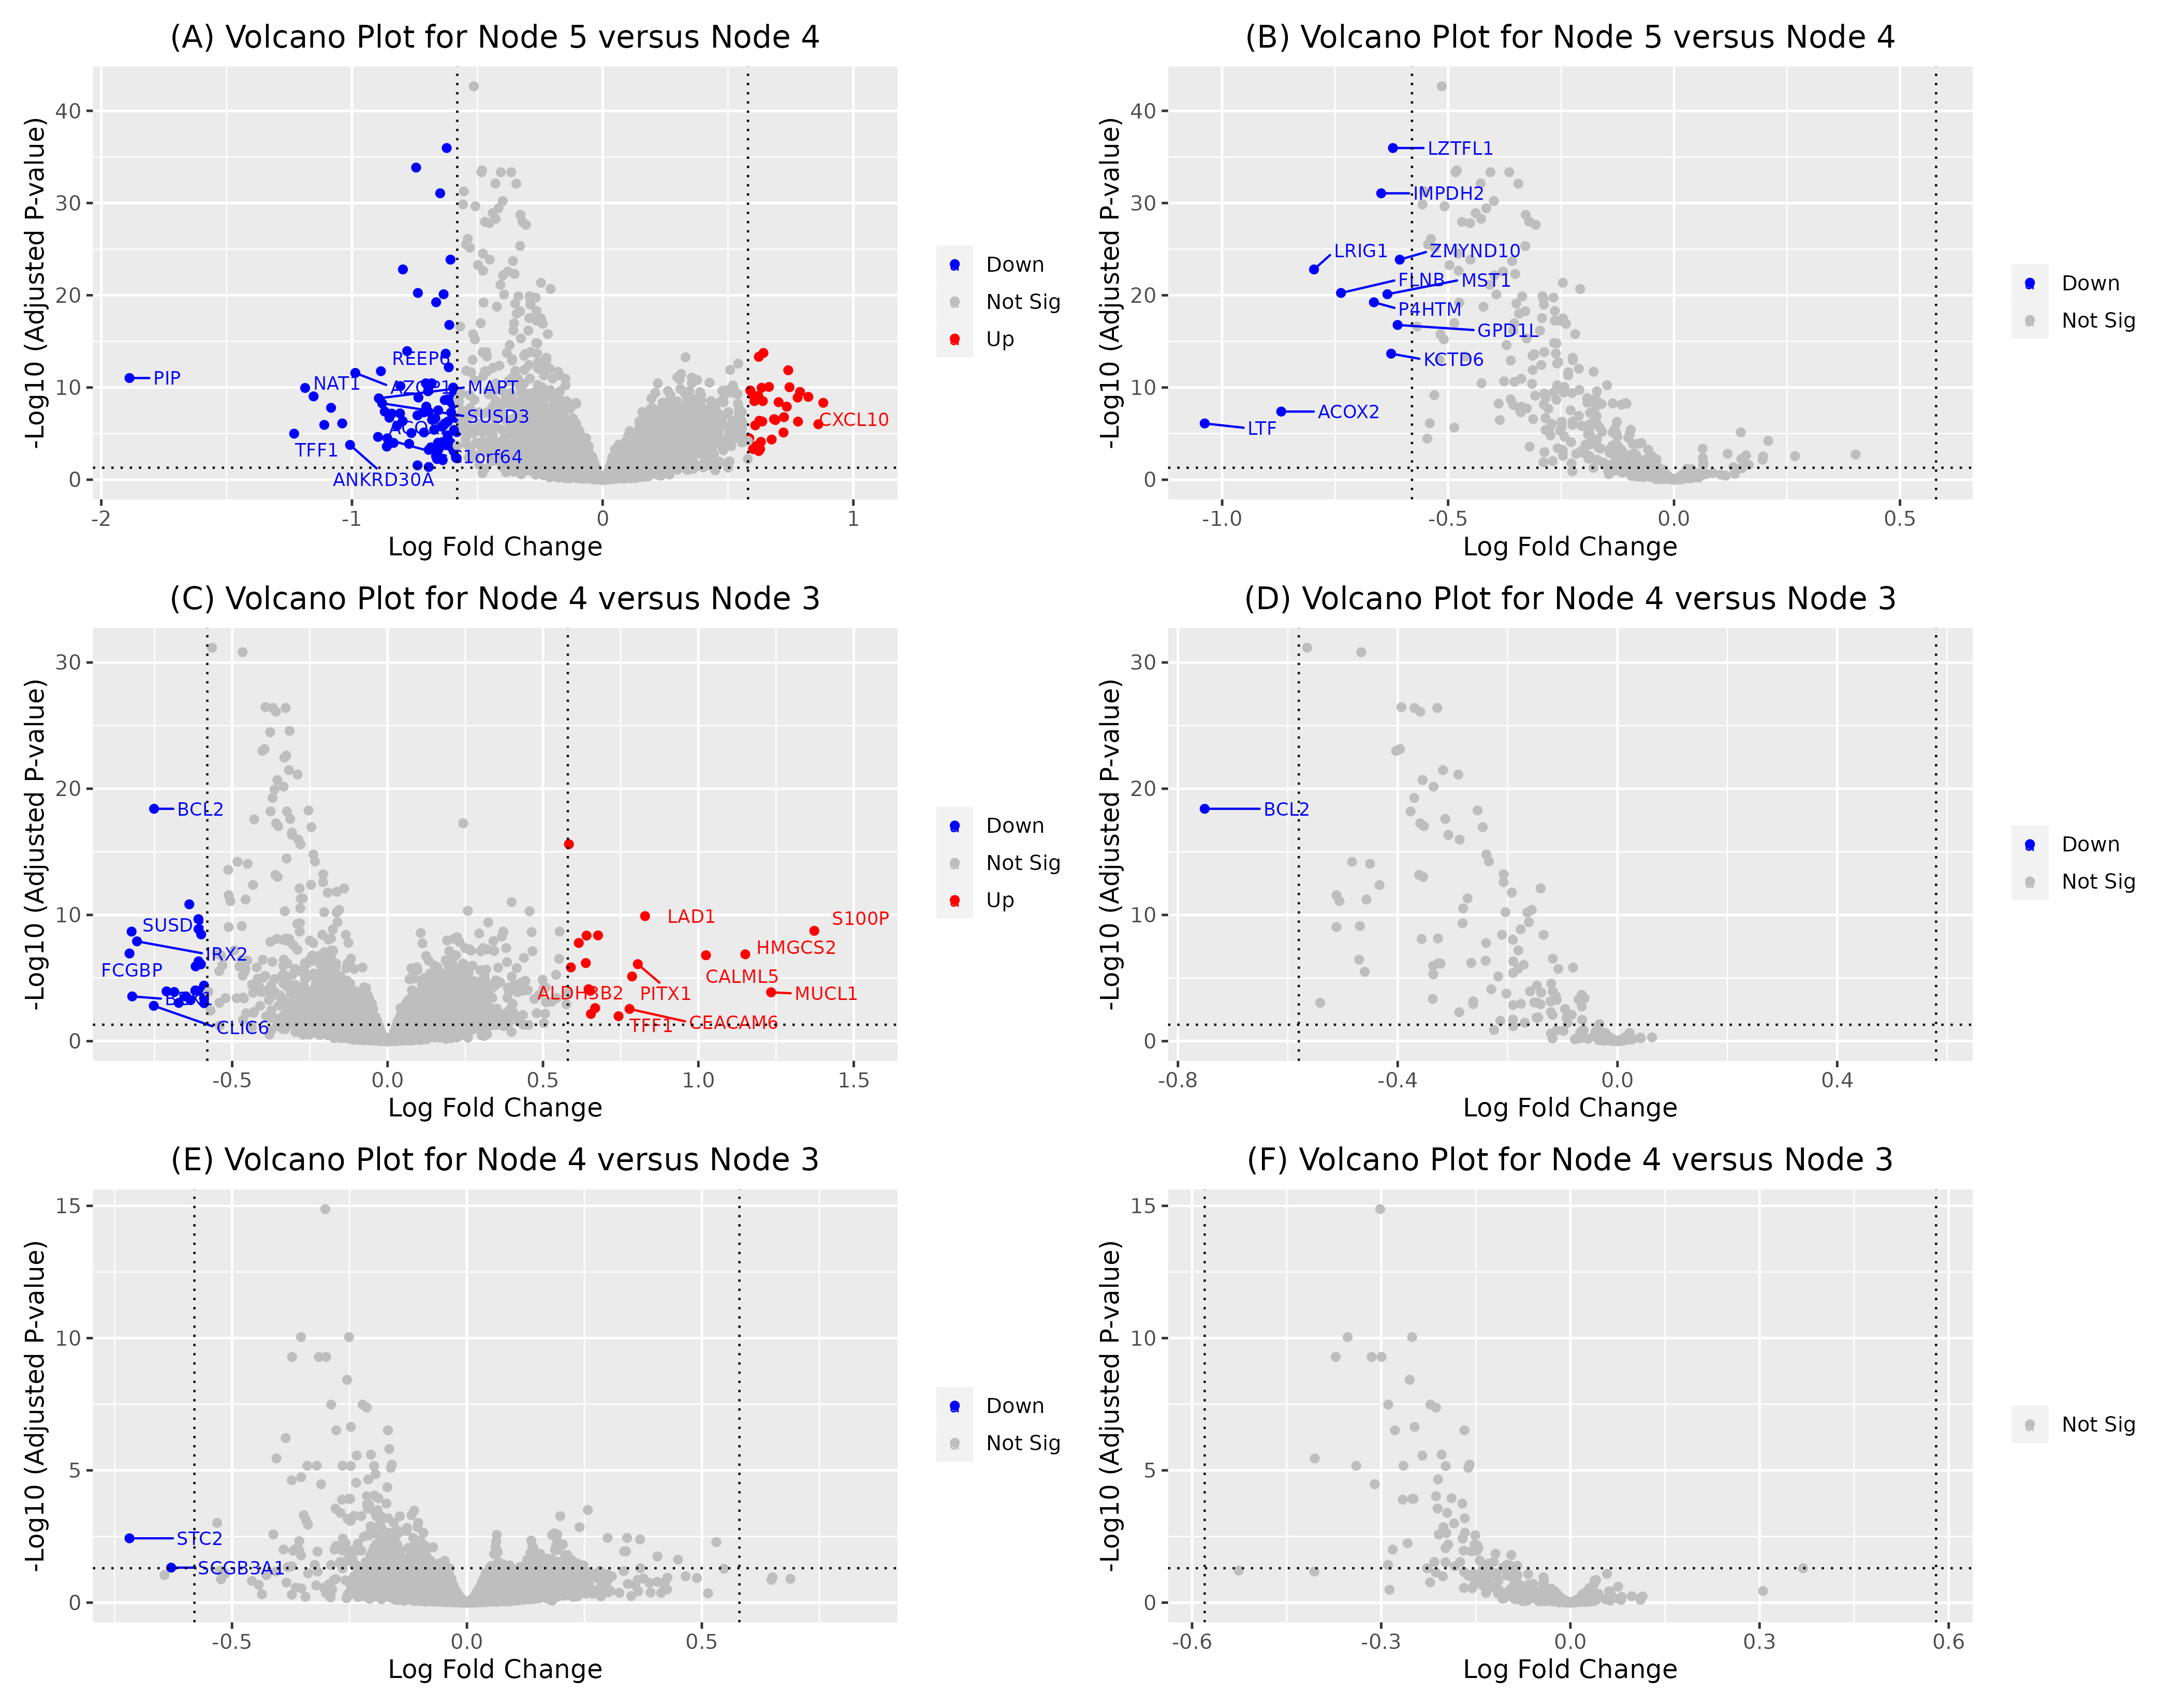
\includegraphics[width=1\linewidth]{../figures/Chapter_4/Volcano_Chr_Total.png}
\caption[Volcano plots resulting from DGEA applied to compare Nodes informed by chromosome arm specific CNA Burden metrics.]{Volcano plots resulting from DGEA applied to compare Nodes informed by chromosome arm specific CNA Burden metrics. Plots show differentially expressed genes between: (A) Node 5 and Node 4 of the ctree DSS survival tree, (C) Node 4 and Node 3 of the rpart 5-year DSS survival tree, and (E) Node 4 and Node 3 of the rpart 10-year DSS survival tree. Plots (B), (D) and (F) correspond to plots (A), (C) and (E), but only show the genes present on the chromosome arm of interest.}
\label{fig:Volcano_chr_total}
\end{figure}
\vfill

\subsubsection{Differential Gene Expression Analysis of CNA States}
The CNA metrics are a cumulative measure over all genes. To explore the direct relationship between the gene's individual CNA and the gene's expression we propose, fit and use a modified DGEA model. Applications of DGEA using limma usually applies the same design matrix for all genes:

$$\mathbf{\text{Gene Expression}}_{g} = \mathbf{X} \mathbf{\beta}_{g} + \mathbf{\epsilon}_{g}$$ 

where $\textbf{X}$ is the design matrix and is the same for each gene $g$, $\beta$ is the vector of parameters and $\epsilon$ is the error vector. However, when the CNA states of the gene is the explanatory variable, a patient may have different CNA states for different genes, requiring gene-specific model design matrices. For example, patient MB.0010 may have an amplification (+2) in the gene ACTL8 and should be placed in the amplification group with the other patients displaying an amplification in this gene, but this patient may also have a hemizygous deletion (-1) in the gene MFSD2 and therefore should also be placed in the deletion group with the other patients displaying a deletion in this gene. Here, the CNA state of a gene is one of \textit{amplification, gain, neutral, hemizygous deletion} or \textit{homozygous deletion}, and is considered as predictor in a model with gene expression as the response, proposing the following model specification: 

$$\text{Gene Expression}_{gi} = \beta_{0g} + \beta_{1g}\text{CNA State}_{gi} + \epsilon_{gi}$$ 

where $\text{CNA State}_{gi}$, for gene $g$ and patient $i$, can either take on one of three states, i.e. amplification, neutral or deletion, or one of five states, i.e. amplification, gain, neutral, hemizygous deletion and homozygous deletion, depending on the specification. This five-state specification corresponds to the CNA States assigned by \citep{pmid22522925}. A three-state specification is derived from this, grouping hemizygous and homozygous deletions together, and gains and amplifications together. 

Focusing first on the three-state model specification, and the contrast of patients who exhibit a CNA Amplification in a particular gene, to those who exhibit no alteration, CNA Neutral, 772 genes including GRB7, ERBB2 (HER2) and PGAP3, are significantly up-regulated for the amplification state (Figure \ref{fig:Volcano3}A). Comparing the expression of genes with CNA Deletions to genes without alteration, CNA Neutral, 362 genes are differentially expressed (Figure \ref{fig:Volcano3}C). In this case, 345 are down-regulated, including FOXA1, IL6ST and EEF1A2. These plots suggests that the presence of a CNA in a gene has the potential to impact the expression of that gene. Figure \ref{fig:Volcano4}A, B, C and D show that in the five-state specification many genes that have a gain or amplification present are significantly up-regulated, while Figure \ref{fig:Volcano4}E, F, G and H show that in the five-state specification many genes that have a hemizygous or homozygous deletion present are significantly down-regulated. 

The number of genes filtered out of the three-state model results, comparing patients who exhibit a CNA Deletion in a particular gene, to those who exhibit no alteration (i.e. CNA Neutral) is low (418 out of 18,739 filtered from the results). Similarly, the number of genes filtered out of the three-state model results, comparing patients who exhibit a CNA Amplification in a particular gene, to those who exhibit no alteration (i.e. CNA Neutral) is also negligible with 99 genes out of 18,739 being filtered from the results. However, in the five-state specification the impact of small sample size alteration groups is much more pronounced, particularly in the amplification and homozygous deletion groups. The number of genes filtered out when comparing the CNA Gain to CNA Neutral group, CNA Amplification to CNA Neutral group, CNA Hemizygous Deletion to CNA Neutral group and CNA Homozygous Deletion to CNA Neutral group are 129, 9,780, 422 and 18,617, respectively.  

Two gene sets, ModLim3 and ModLim5, containing differentially expressed genes of sufficiently large sample size, i.e. genes with an adjusted p-value below 0.05 and absolute log fold change above 0.58 in at least one contrast, in the three- and five-state specification are defined. 

\vfill 
\begin{figure}[!h]
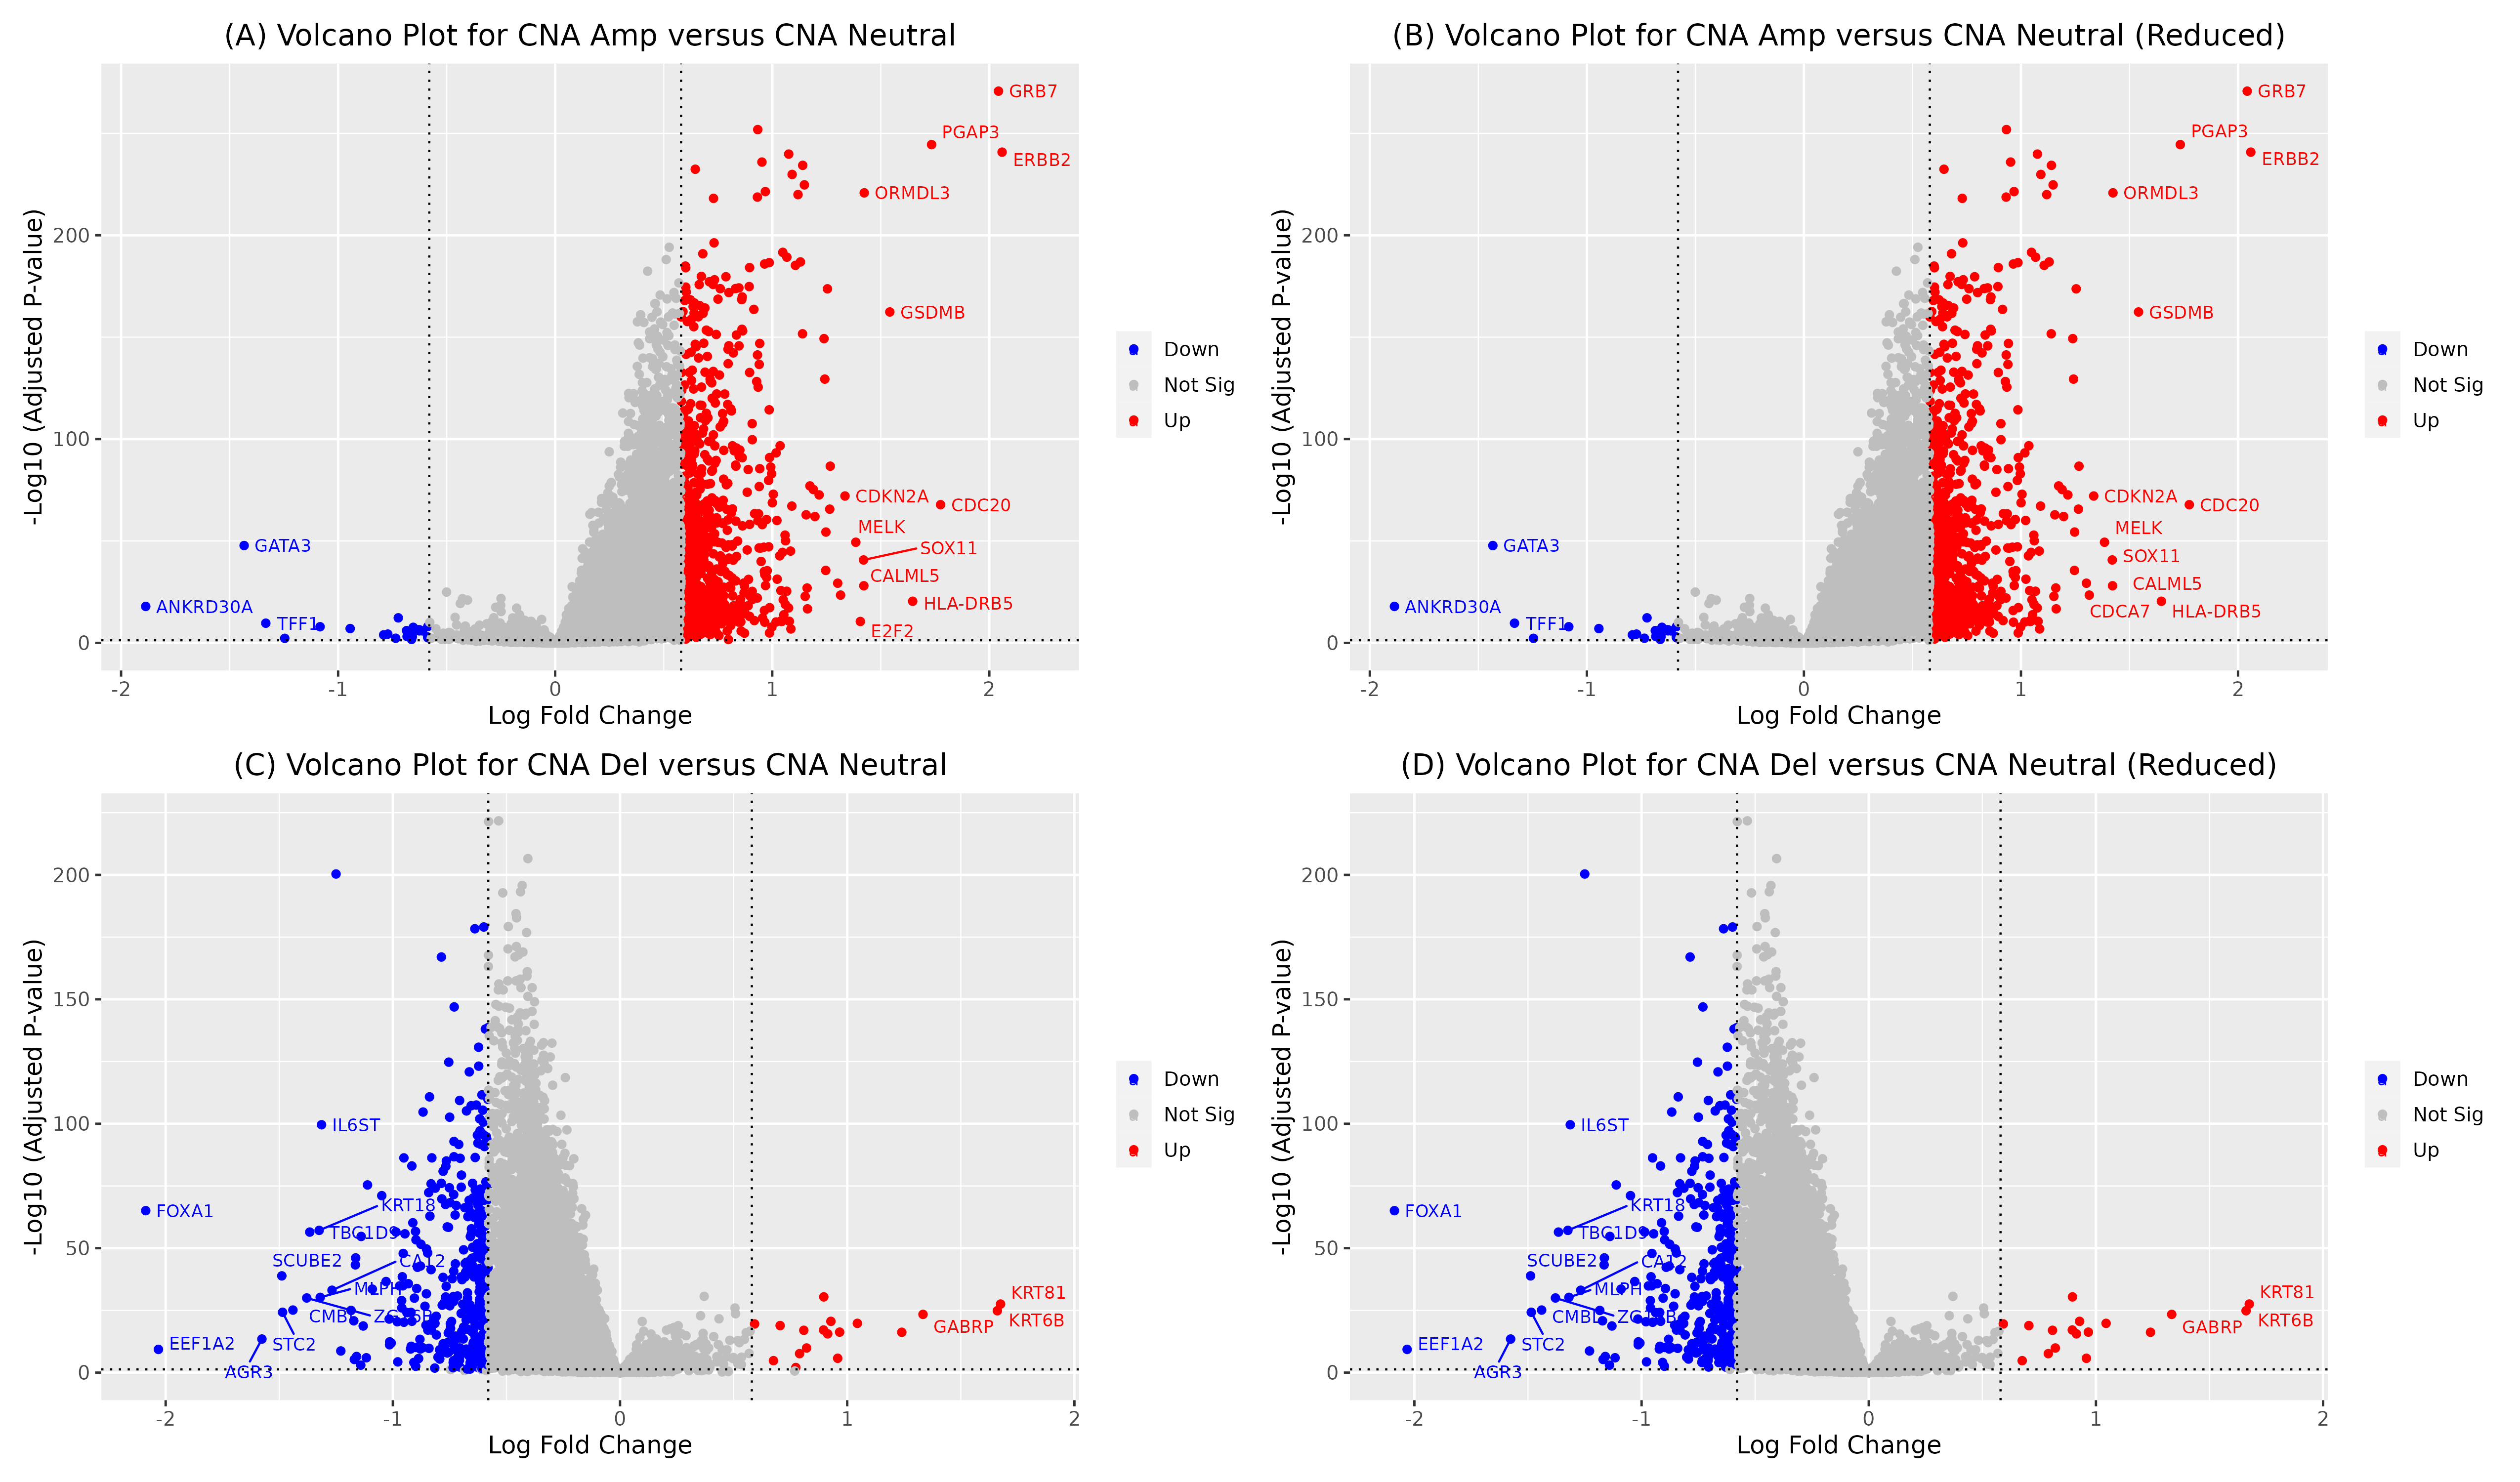
\includegraphics[width=1\textwidth]{../figures/Chapter_4/Volcano_CNA_3State.png}
\caption[Volcano plot showing differentially expressed genes comparing CNA three-state specifications.]{Volcano plot showing differentially expressed genes comparing CNA three-state specifications. Plots denote (A) the CNA Amplification and CNA Neutral states, where all genes are shown (B) the CNA Amplification and CNA Neutral states, where only the genes displaying sufficient numbers of patients with an amplification are shown (C) the CNA Deletion and CNA Neutral states, where all genes are shown (D) the CNA Deletion and CNA Neutral states, where only the genes displaying sufficient numbers of patients with an deletion are shown.}
\label{fig:Volcano3}
\end{figure}
\vfill 

\vfill 
\begin{figure}[!h]
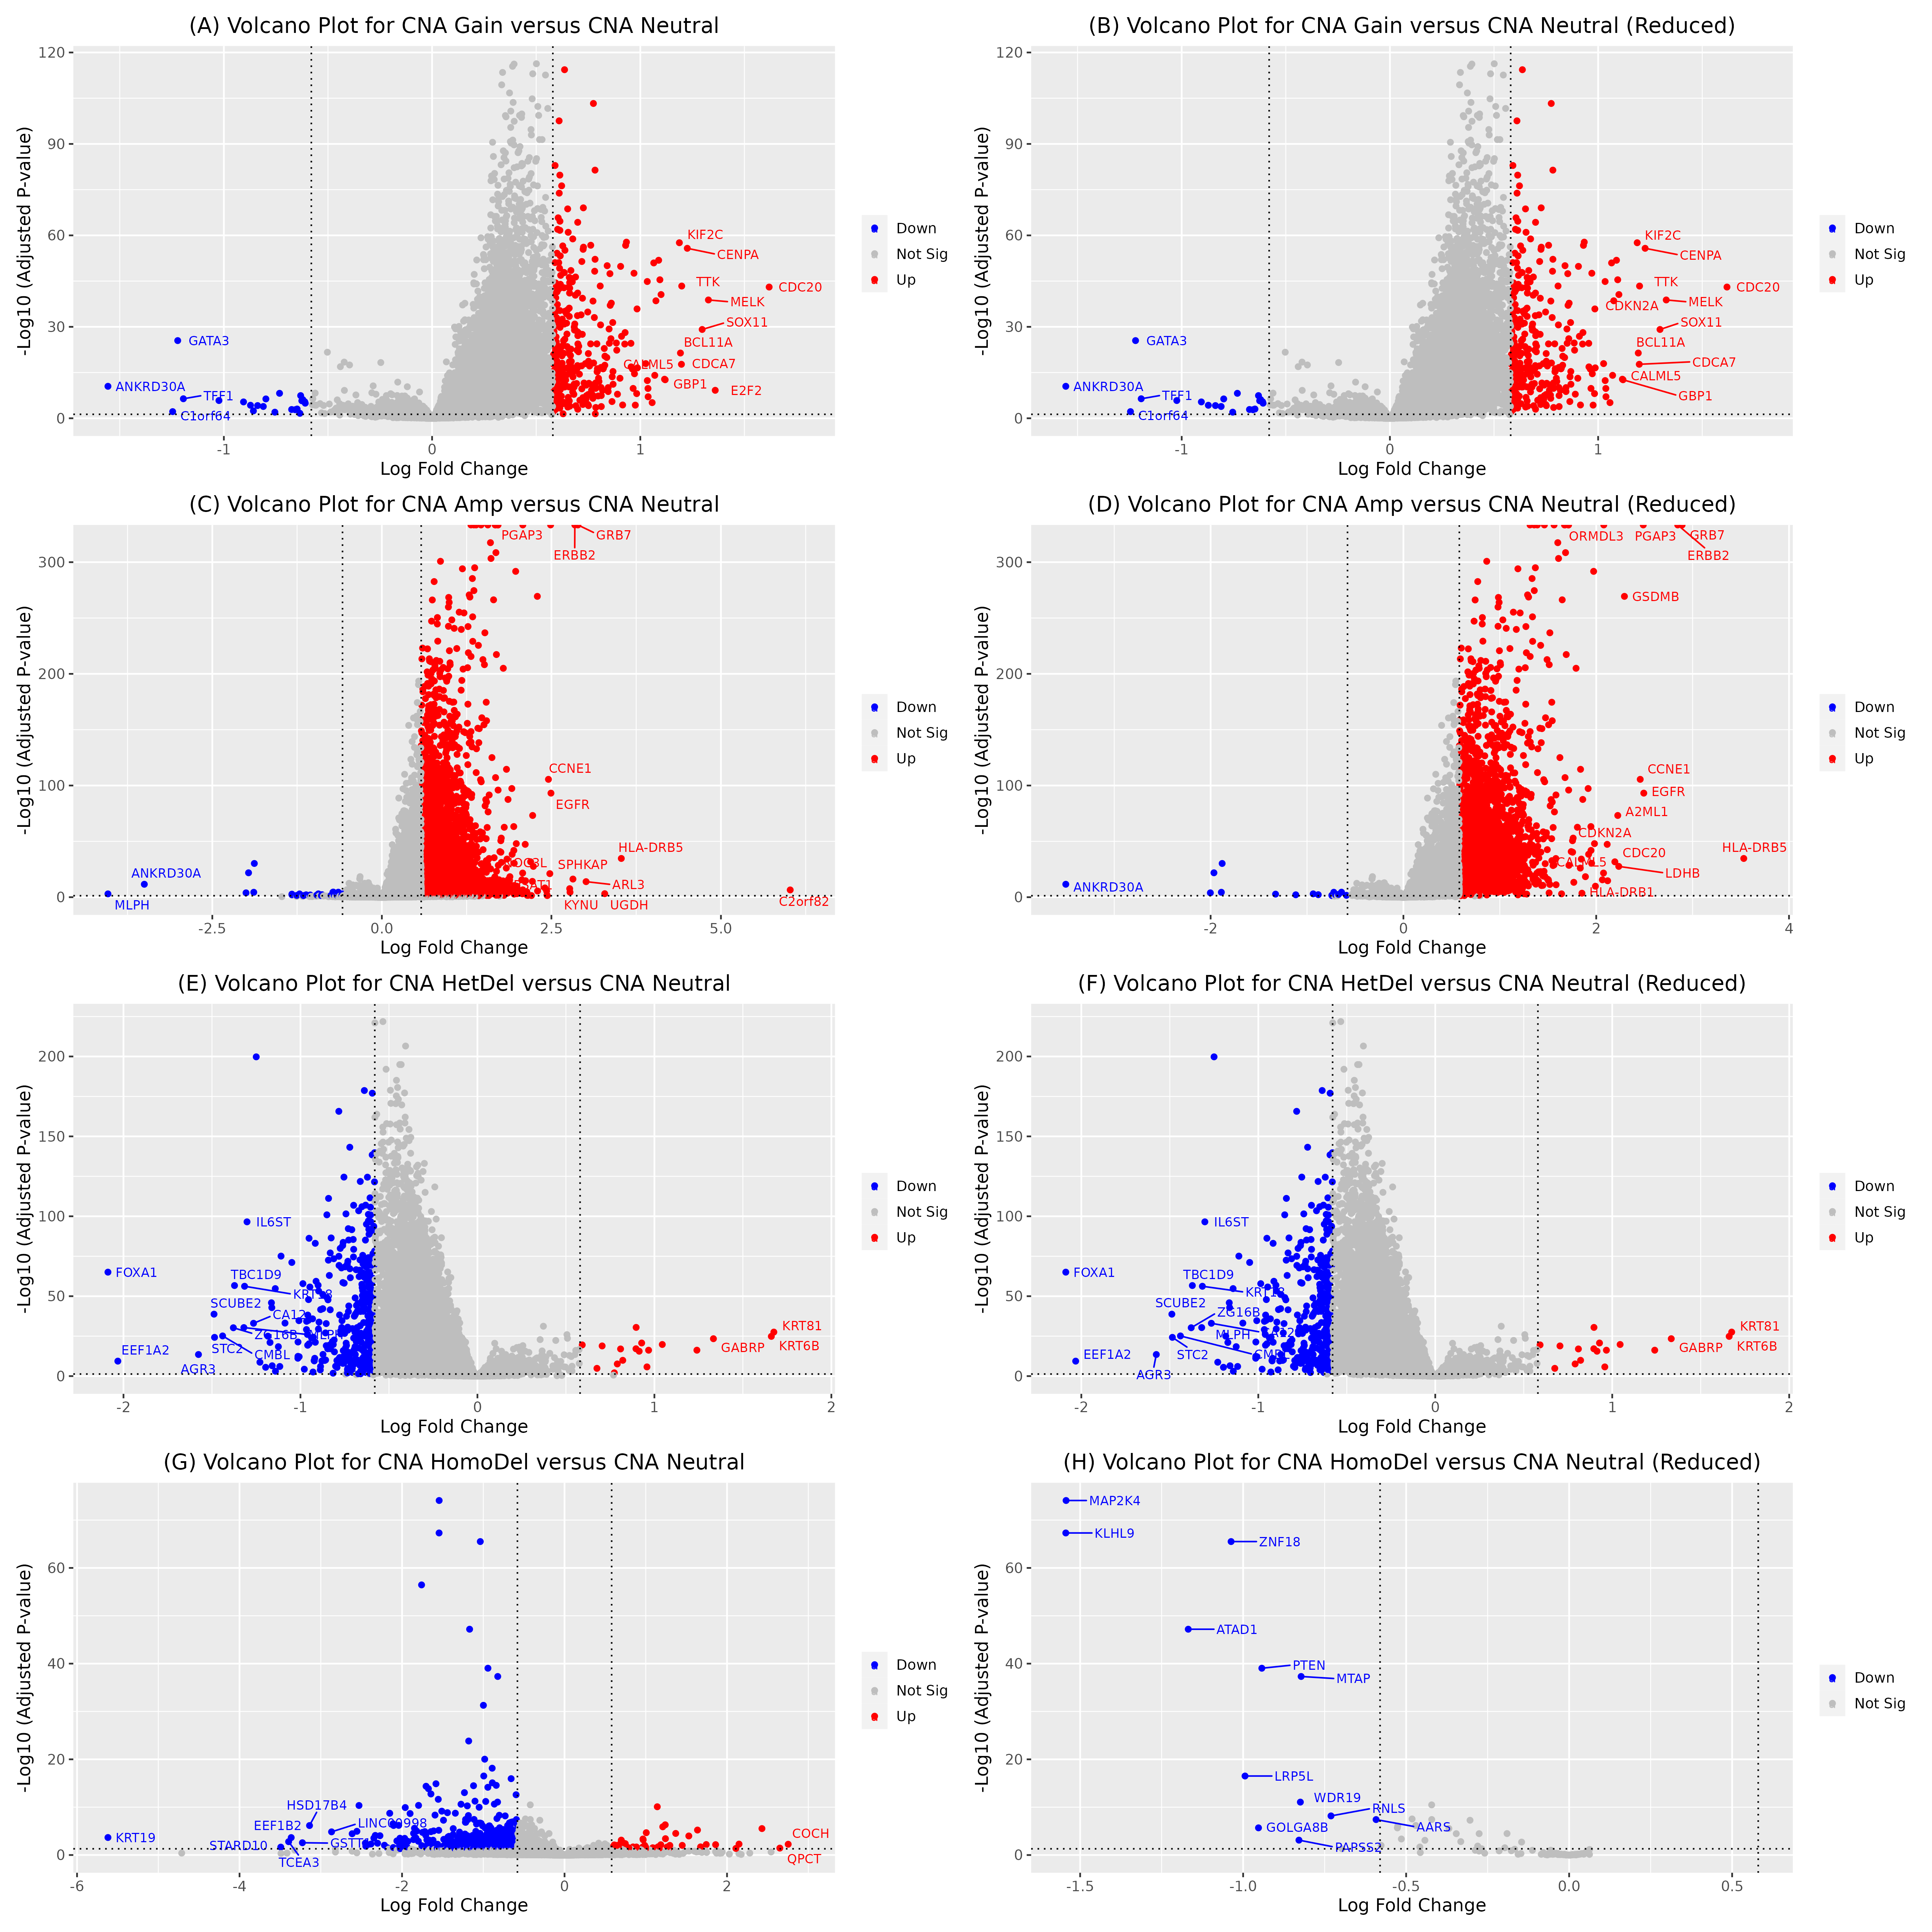
\includegraphics[width=1\textwidth]{../figures/Chapter_4/Volcano_CNA_5State.png}
\caption[Volcano plot showing differentially expressed genes comparing CNA five-state specifications.]{Volcano plot showing differentially expressed genes comparing CNA five-state specifications. Plots denote (A) the CNA Gain and CNA Neutral states, where all genes are shown (C) the CNA Amplification and CNA Neutral, where all genes are shown (E) the CNA Hemizygous Deletion and CNA Neutral states, where all genes are shown and (G) the CNA Homozygous Deletion and CNA Neutral states, where all genes are shown. Figures (B), (D), (F) and (H) correspond to (A), (C), (E) and (G), where only the genes displaying sufficient numbers of patients with a CNA are shown.}
\label{fig:Volcano4}
\end{figure}
\vfill 
\clearpage
\subsection{Comparative Study}
To explore the level of congruence and whether new gene identifications arise in our ModLim3 and ModLim5 differentially expressed gene sets, a comparative study is conducted against some established molecular classification, prognostic and predictive assays reported in the literature. The prognostic and predictive assays selected for comparison are Oncotype DX, MammaPrint, Prosigna (PAM50) and BCI, and molecular classifications, PAM50 and IntClust.

Oncotype DX is a reverse transcription polymerase chain reaction (RT-PCR) based 21 gene signature used to predict the probability of disease recurrence and to help identify patients who are likely to benefit from adjuvant chemotherapy. Of these 21 genes, 16 are linked to cancer and 5 are used as controls (see Appendix C). The expression of these 21 genes is measured and based on the relative expression of the cancer associated genes to the control genes, a score called recurrence score is calculated. This recurrence score, which ranges from 0 to 100, categorises patients into 3 subgroups. Patients with recurrence score less than 18 are assigned as low risk of recurrence, patients with recurrence score 18-30 are assigned as intermediate risk of recurrence and patients with recurrence score greater than 30 are assigned as high risk of recurrence \citep{pmid15591335, pmid28882552}. 

MammaPrint is a microarray-based assay that predicts the probability of disease recurrence and helps guide treatment decision making in breast cancer patients \citep{pmid11823860, pmid12490681, pmid20204499, pmid28882552}. This assay uses the combined expression of 70 genes (the Amsterdam 70-gene expression profile, Appendix C) to categorise tumours as low or high risk for disease recurrence or metastasis. MammaPrint can be used as a prognostic and predictive biomarker in patients with newly diagnosed lymph node-negative or lymph node-positive (1-3 metastatic nodes) invasive breast cancer. 

The Prosigna test, formerly known as PAM50, is a microarray-based assay that predicts the probability of disease recurrence, helps guide treatment decision making in hormone-receptor-positive, HER2-negative breast cancer patients and can classify breast cancers into intrinsic molecular subtypes. The assay measures the expression of 58 genes; the 50 PAM50 genes and eight control genes for normalisation (see Appendix C). Based on the relative expression of these genes, a risk score ranging from 0-100 is produced. Using this risk score, patients with node-negative breast cancer are split into low (0-40), intermediate (41-60), or high risk (61-100) categories, while node-positive breast cancer patients are split into low (0-40) or high risk (41-100) categories \citep{DUFFY2017284, pmid28882552}.   

BCI is a microarray-based assay that predicts outcome and helps guide adjuvant treatment decision making in lymph node-negative, HR+ and HER2- patients. This assay measures the expression of 11 genes, 7 test genes and 4 control genes (see Appendix C). The development of this assay was based on the combination of two previously identified molecular assays, the HOXB13:IL17BR ratio and the Molecular Grade Index. The HOXB13:IL17BR ratio is a two-gene expression assay that can predict disease-free survival in early-stage breast cancer \citep{pmid15193263} and the Molecular Grade Index is a five-gene expression assay, comprising genes related to histological grade and tumour progression that helps predict risk of distant metastasis in ER+, lymph node-negative patients \citep{pmid18451222}.  

Table \ref{Tab:Tcr} provides information on the number of genes measured within each assay/molecular classification and any differences in availability compared to the processed METABRIC CNA and gene expression data, while Figures \ref{fig:VD_Compare} and \ref{fig:lo} provide results of comparative study.

High congruence is observed when comparing ModLim3 and ModLim5 gene sets (Figure \ref{fig:VD_Compare}). Approximately 92\% of genes identified as differentially expressed in the three-state specification were also differentially expressed in the five-state specification. Owing to this high congruence, focus was given to the ModLim5 gene set and its congruence with established molecular classification, prognostic and predictive gene sets. 

\vfill
\begin{table}[!h]
\caption{Table containing gene set information for each assay and availability in the METABRIC data.}
\resizebox{\textwidth}{!}{
\begin{tabular}{|l|c|c|c|}
\hline
\multicolumn{1}{|c|}{\textbf{Gene Assay}} & \textbf{No. Genes Measured} & \textbf{\thead{No. of genes in METABRIC data in \\ common with comparative assay}} & \textbf{Missing Genes} \\ 
\hline
Oncotype DX & 21 & 21 & - \\ 
\hline
MammaPrint & 70 (66 unique) & 62 & \begin{tabular}[c]{@{}c@{}}
 EBF4 (missing from gene expression data) \\
 SERF1A (missing from gene expression data) \\
 KDM7A (missing from gene expression data) \\
 GPR126 (missing from gene expression and CNA data) \\
 LOC100288906 (missing from gene expression and CNA data) \\
 LOC730018 (missing from gene expression and CNA data) \\
 AA555029\_RC (missing from gene expression and CNA data) \\
 LOC100131053 (missing from gene expression and CNA data)
\end{tabular} \\ 
\hline
PAM50\_Prosigna & 50 (58) & 58 & - \\ 
\hline
BCI & 11 & 11 & - \\ 
\hline
IntClust & 1,000 & 959 & see Appendix D for full list \\ 
\hline
\end{tabular}}
\label{Tab:Tcr}
\end{table}
\vspace{1.5cm}
\begin{figure}[!h]
\centering
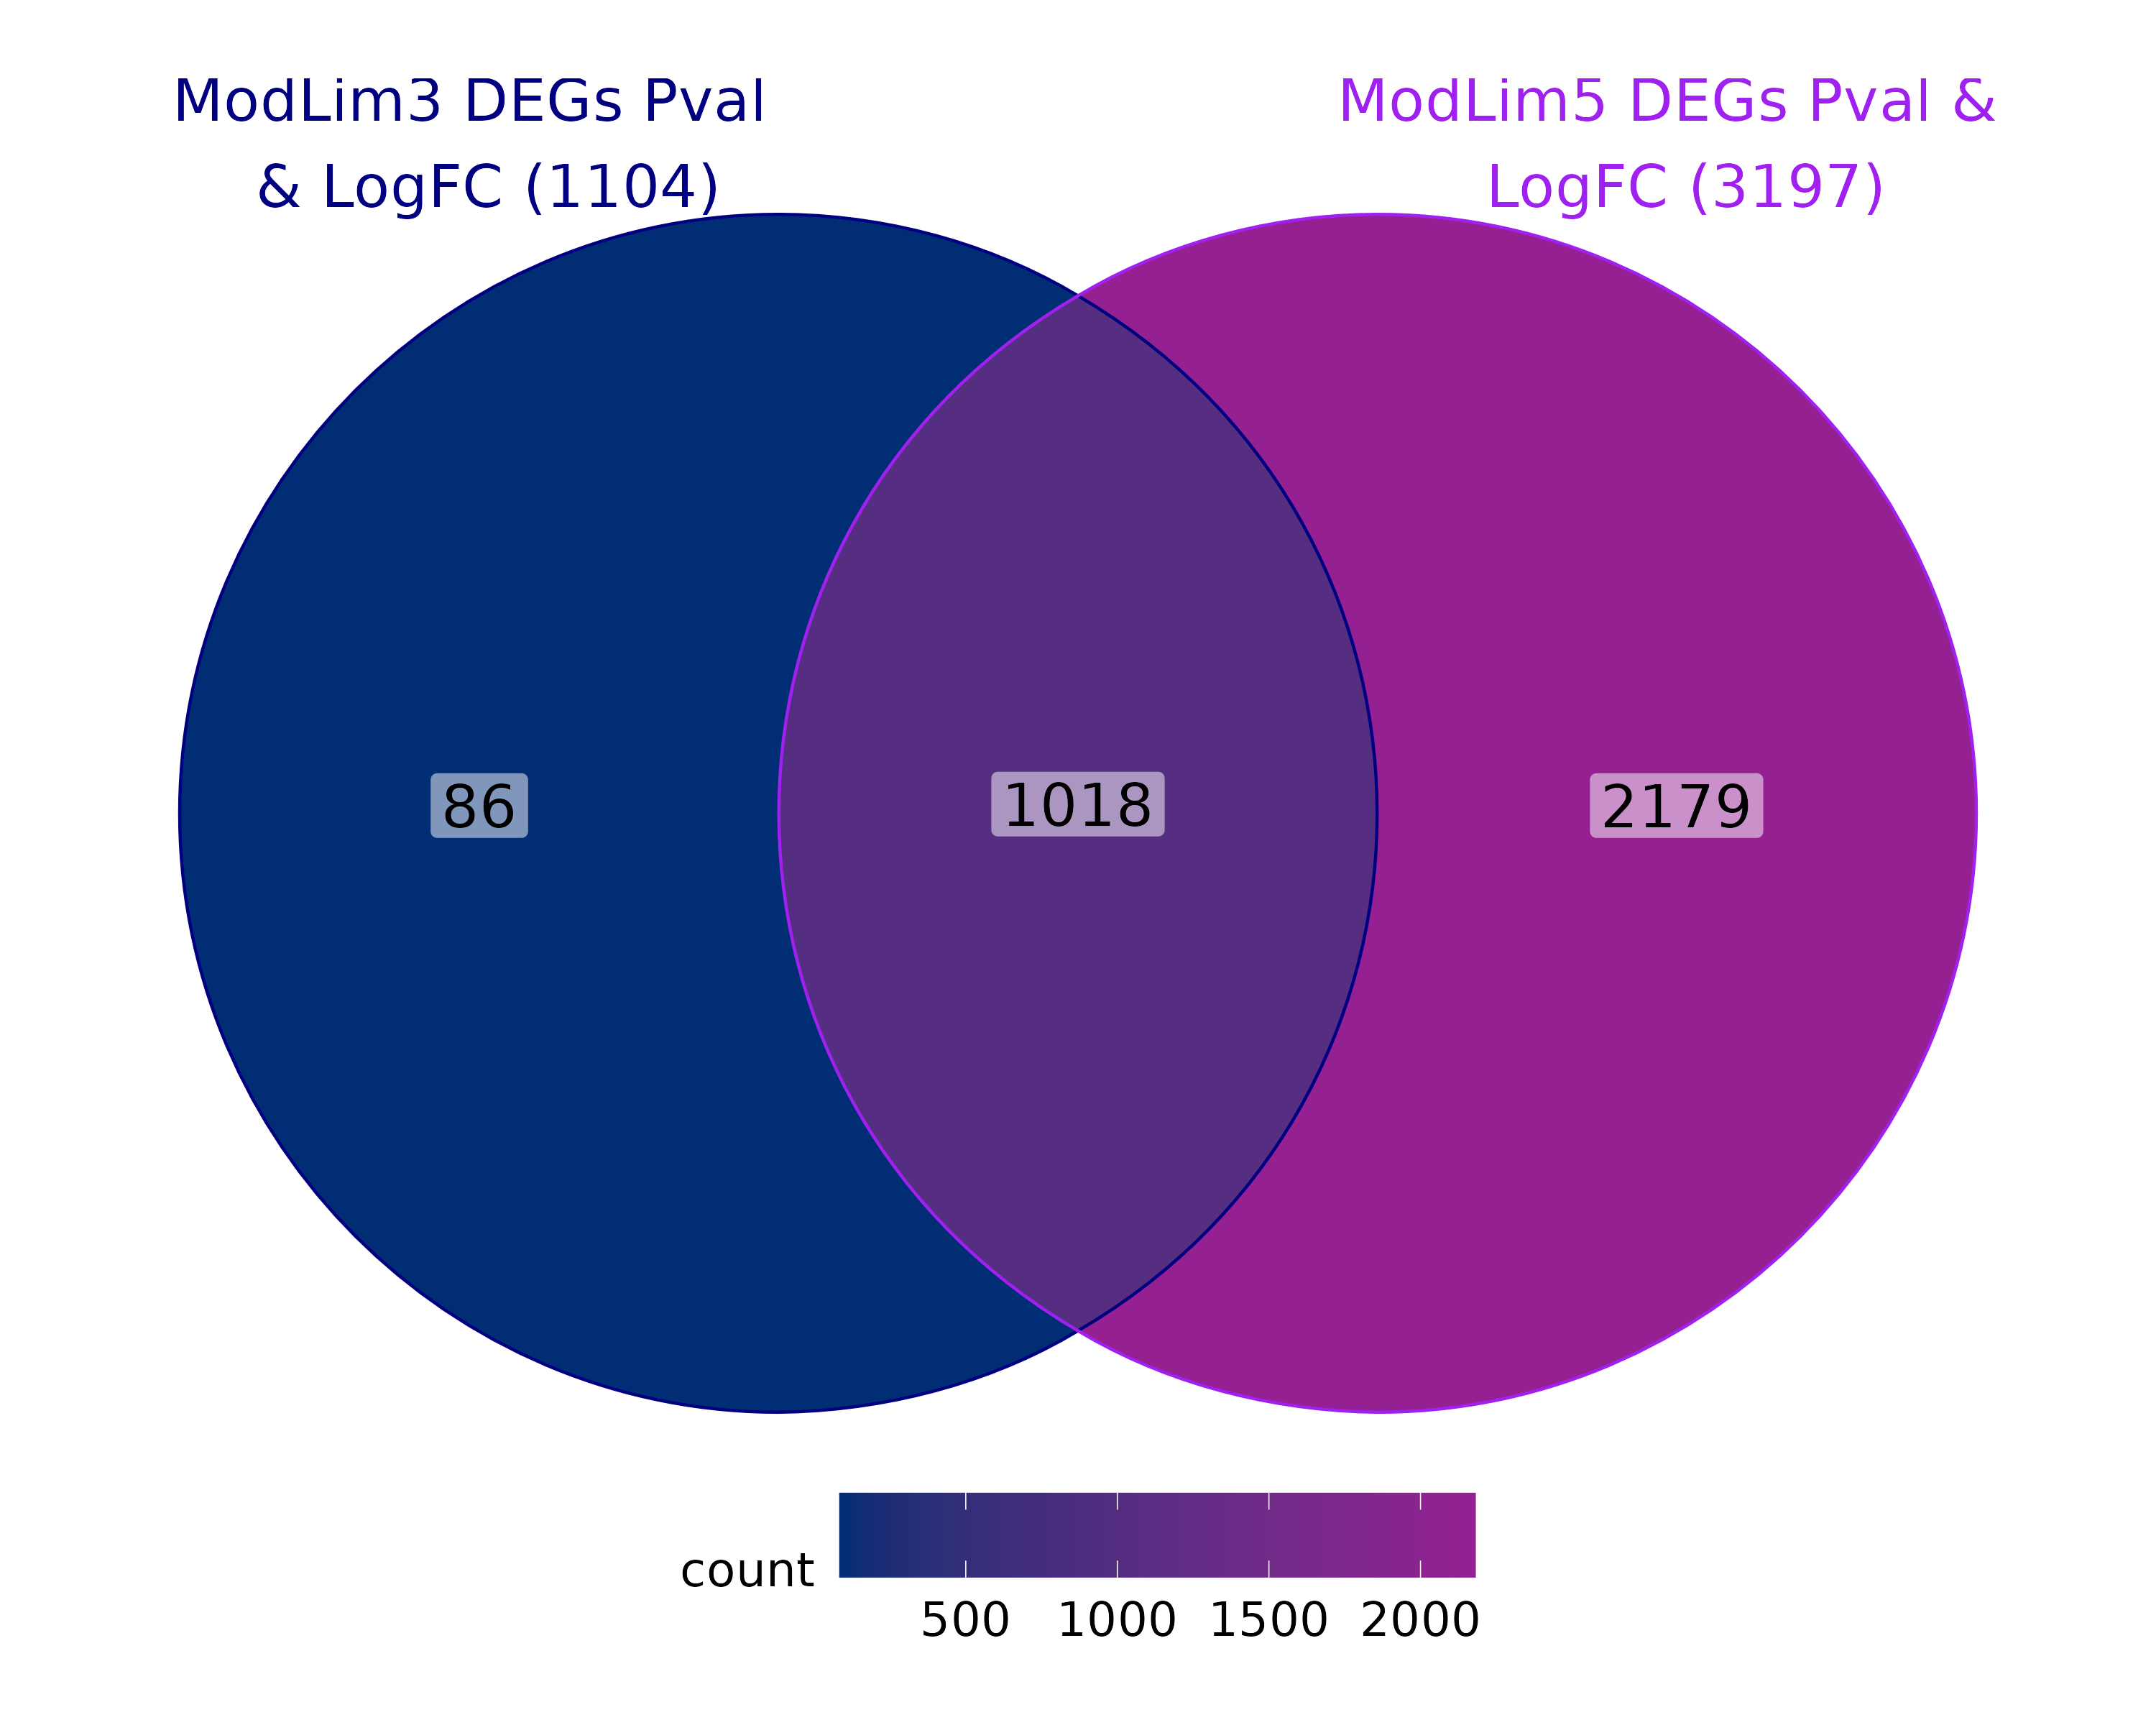
\includegraphics[width=0.7\textwidth]{../figures/Chapter_4/Venn_3State_5State.png}
\caption{Venn diagram showing gene set congruence between the ModLim3 and ModLim5 gene sets.}
\label{fig:VD_Compare}
\end{figure}
\vfill
\newpage 

\captionsetup[subfigure]{font={bf,small}, margin=3.8cm, singlelinecheck=false}

\begin{figure}[H]
\centering

\vspace{1cm}
\subfloat[]{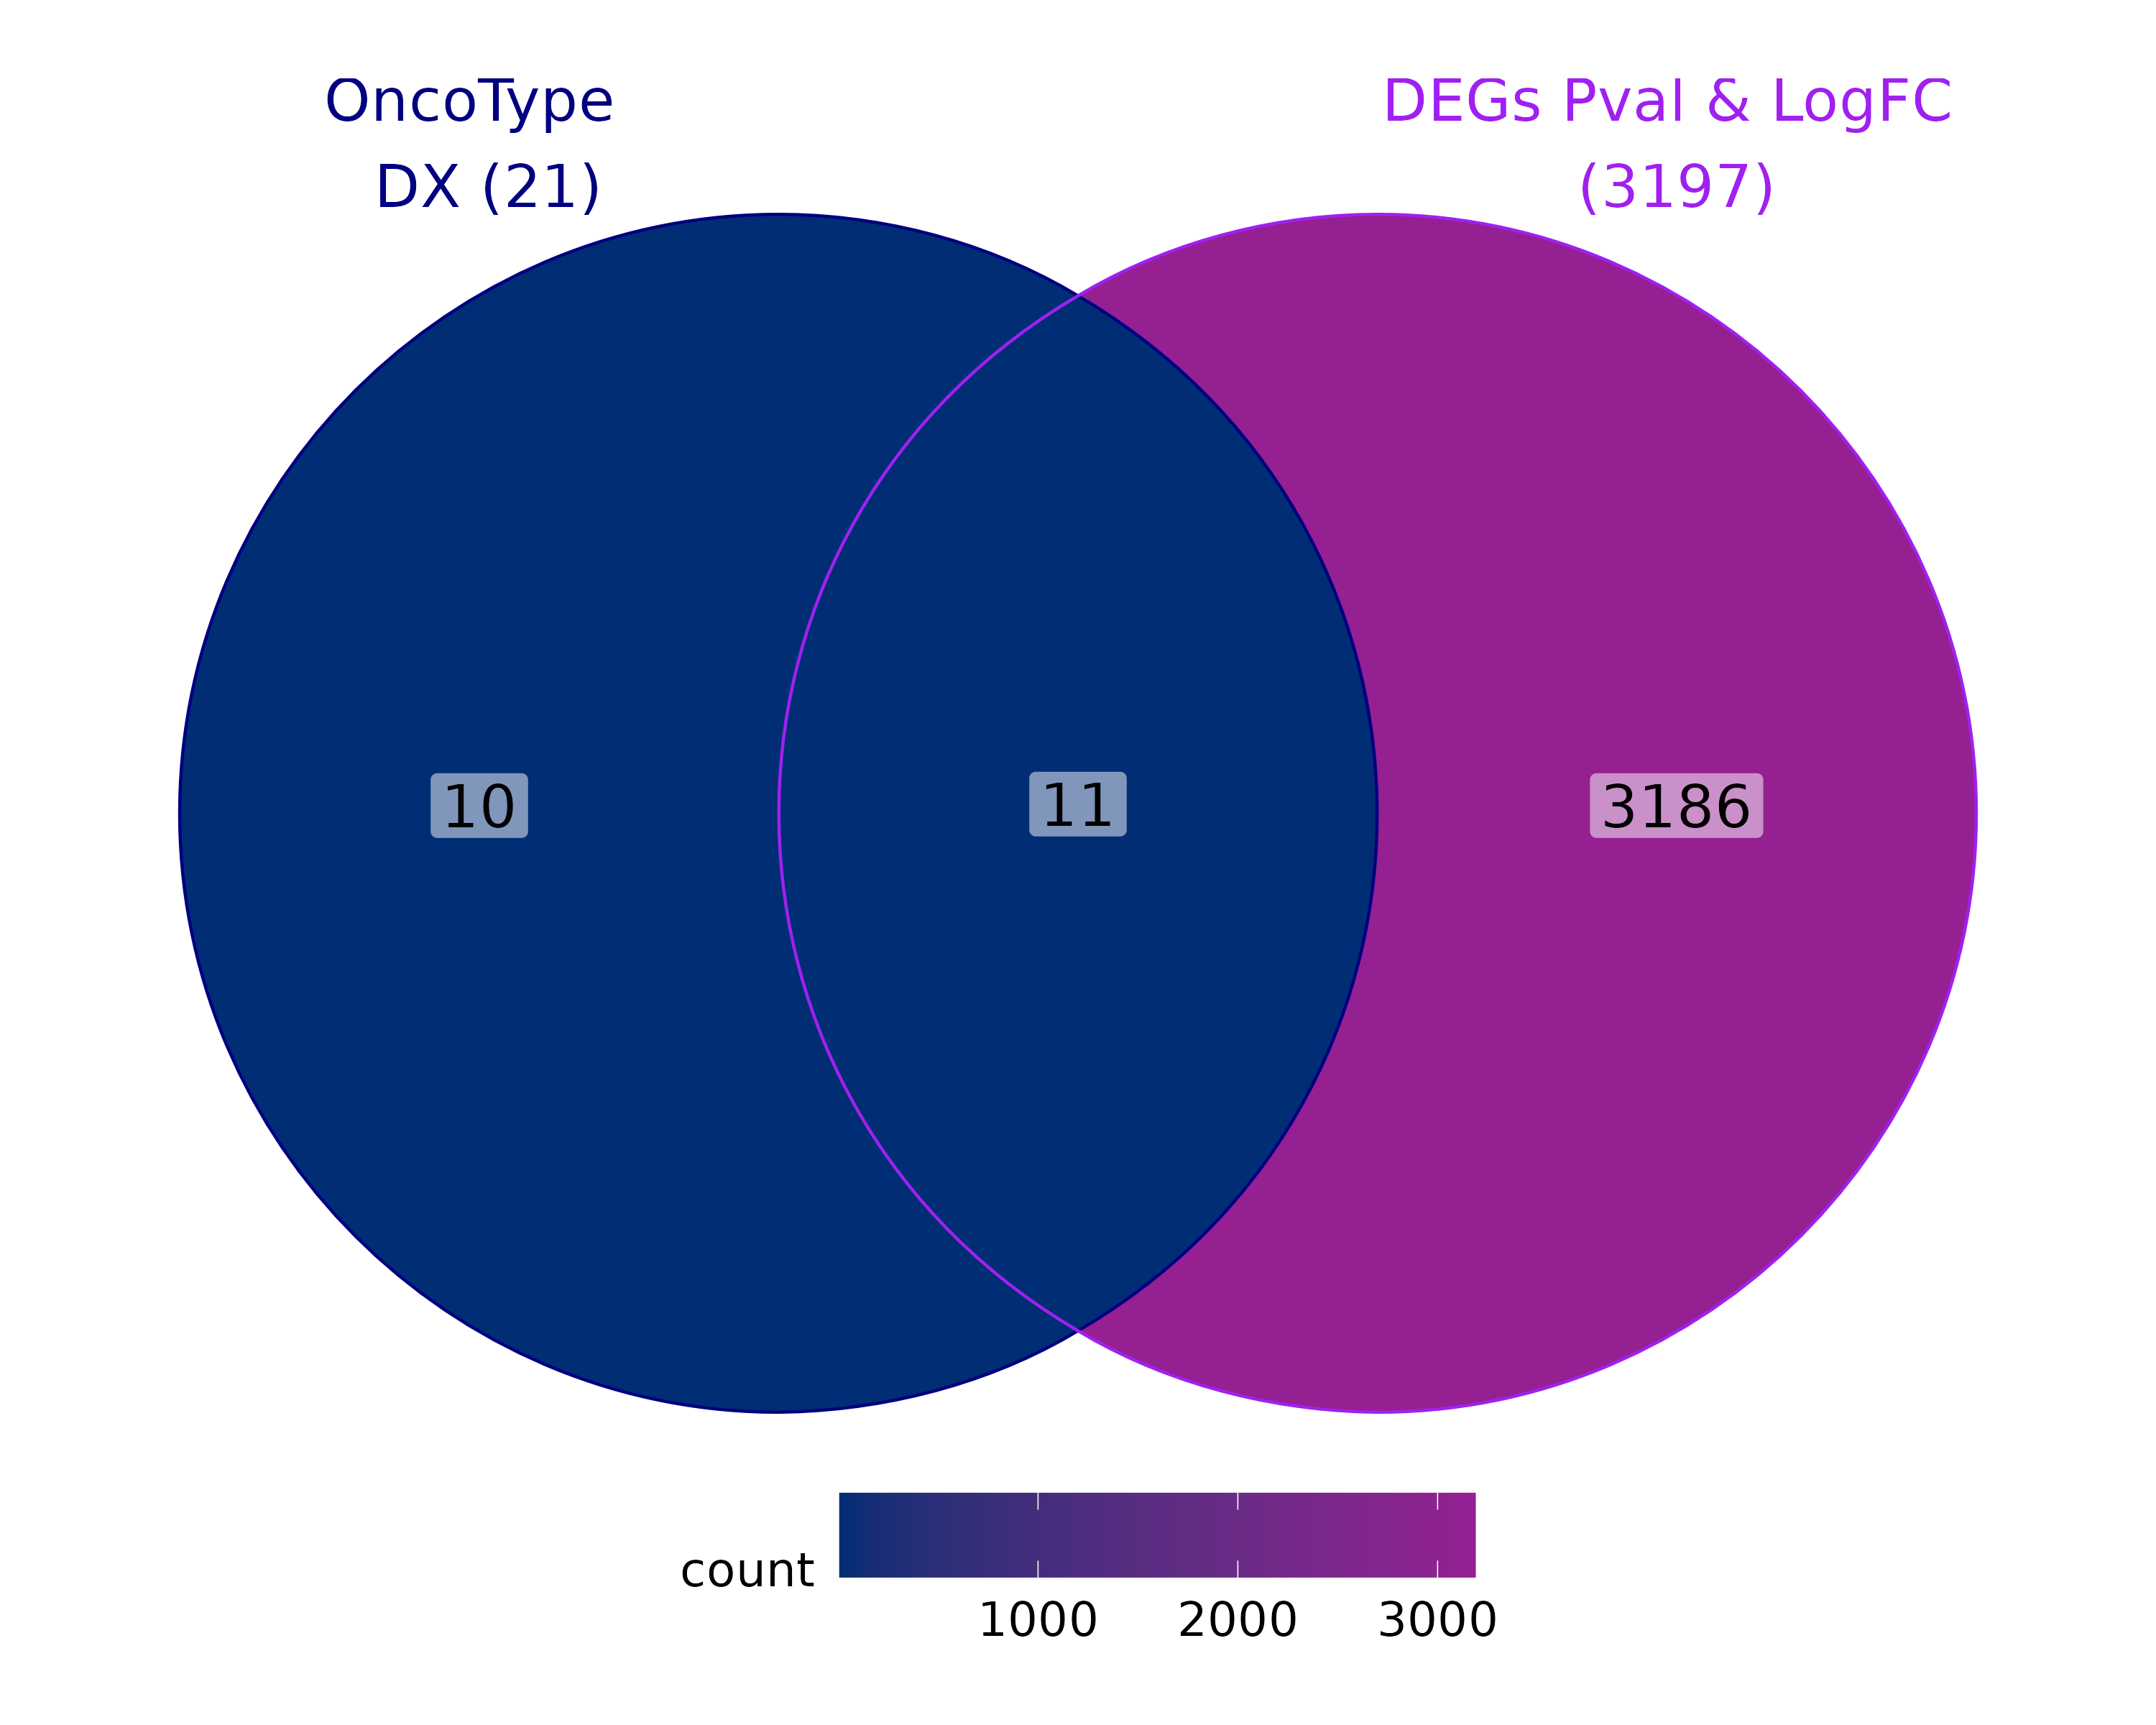
\includegraphics[width=0.5\textwidth]{../figures/Chapter_4/Venn_Onco_Ours.png}}\hfill
\subfloat[]{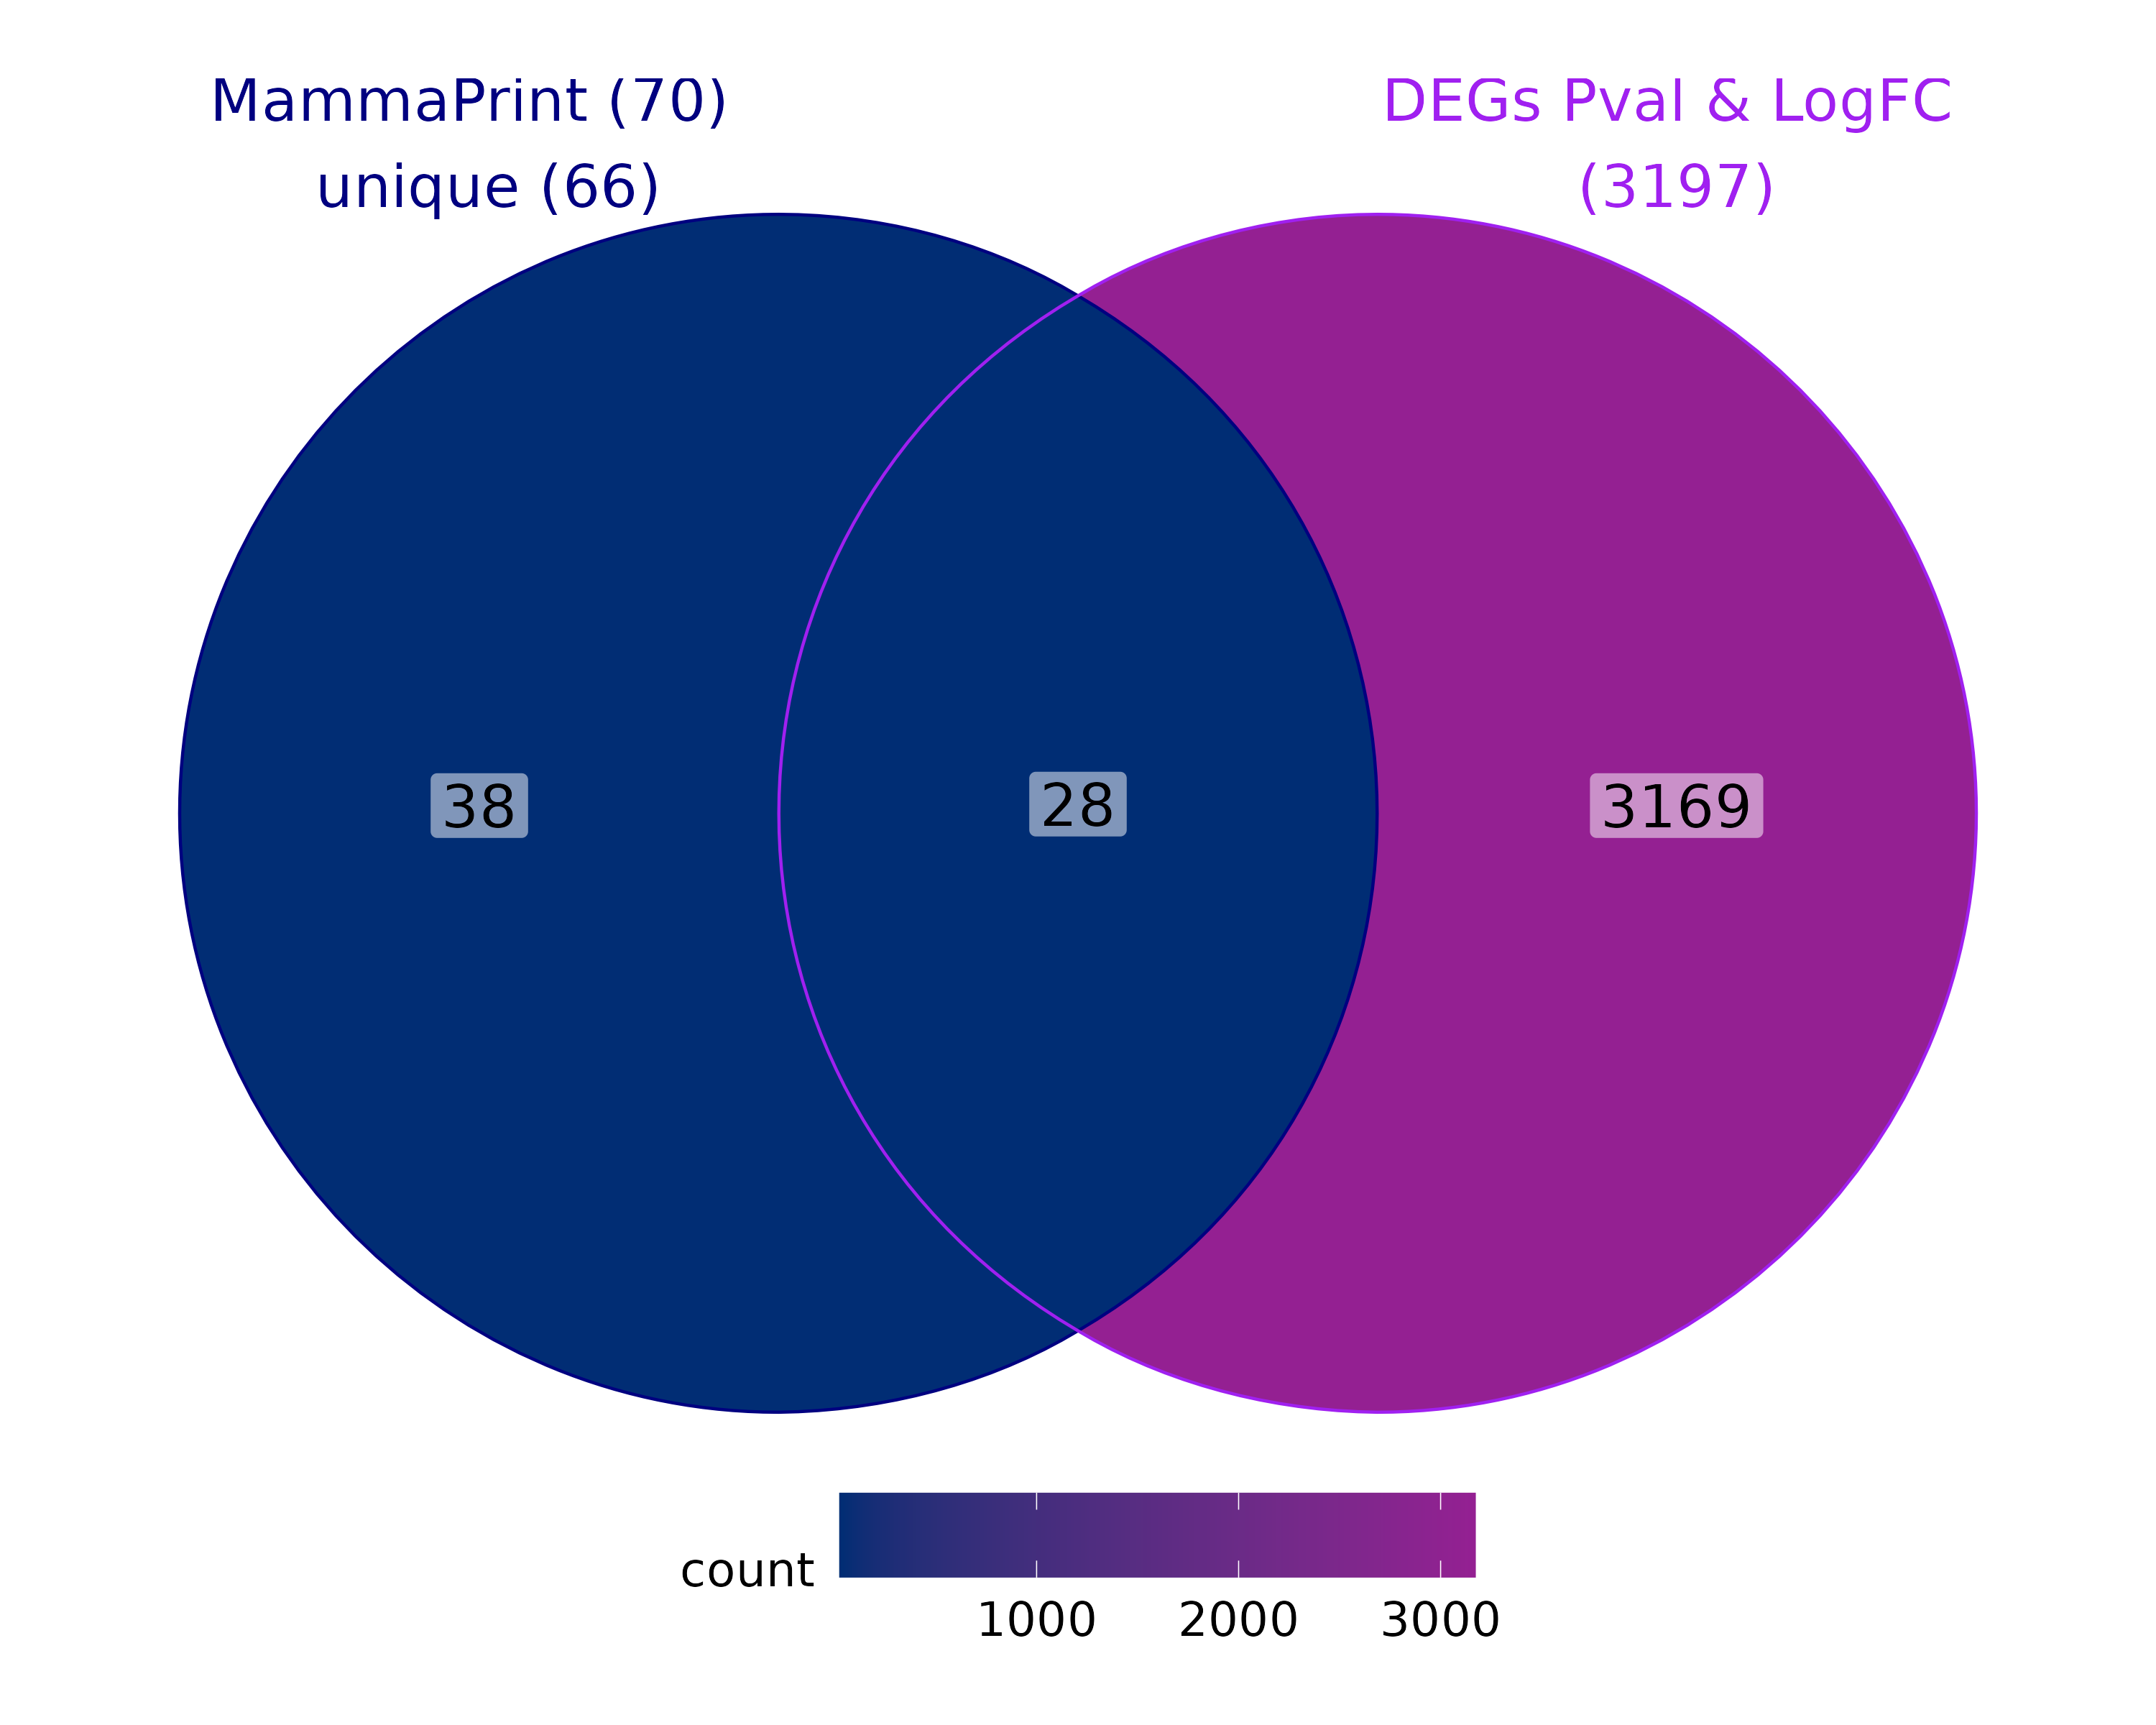
\includegraphics[width=0.5\textwidth]{../figures/Chapter_4/Venn_Mamma_Ours.png}}

\subfloat[]{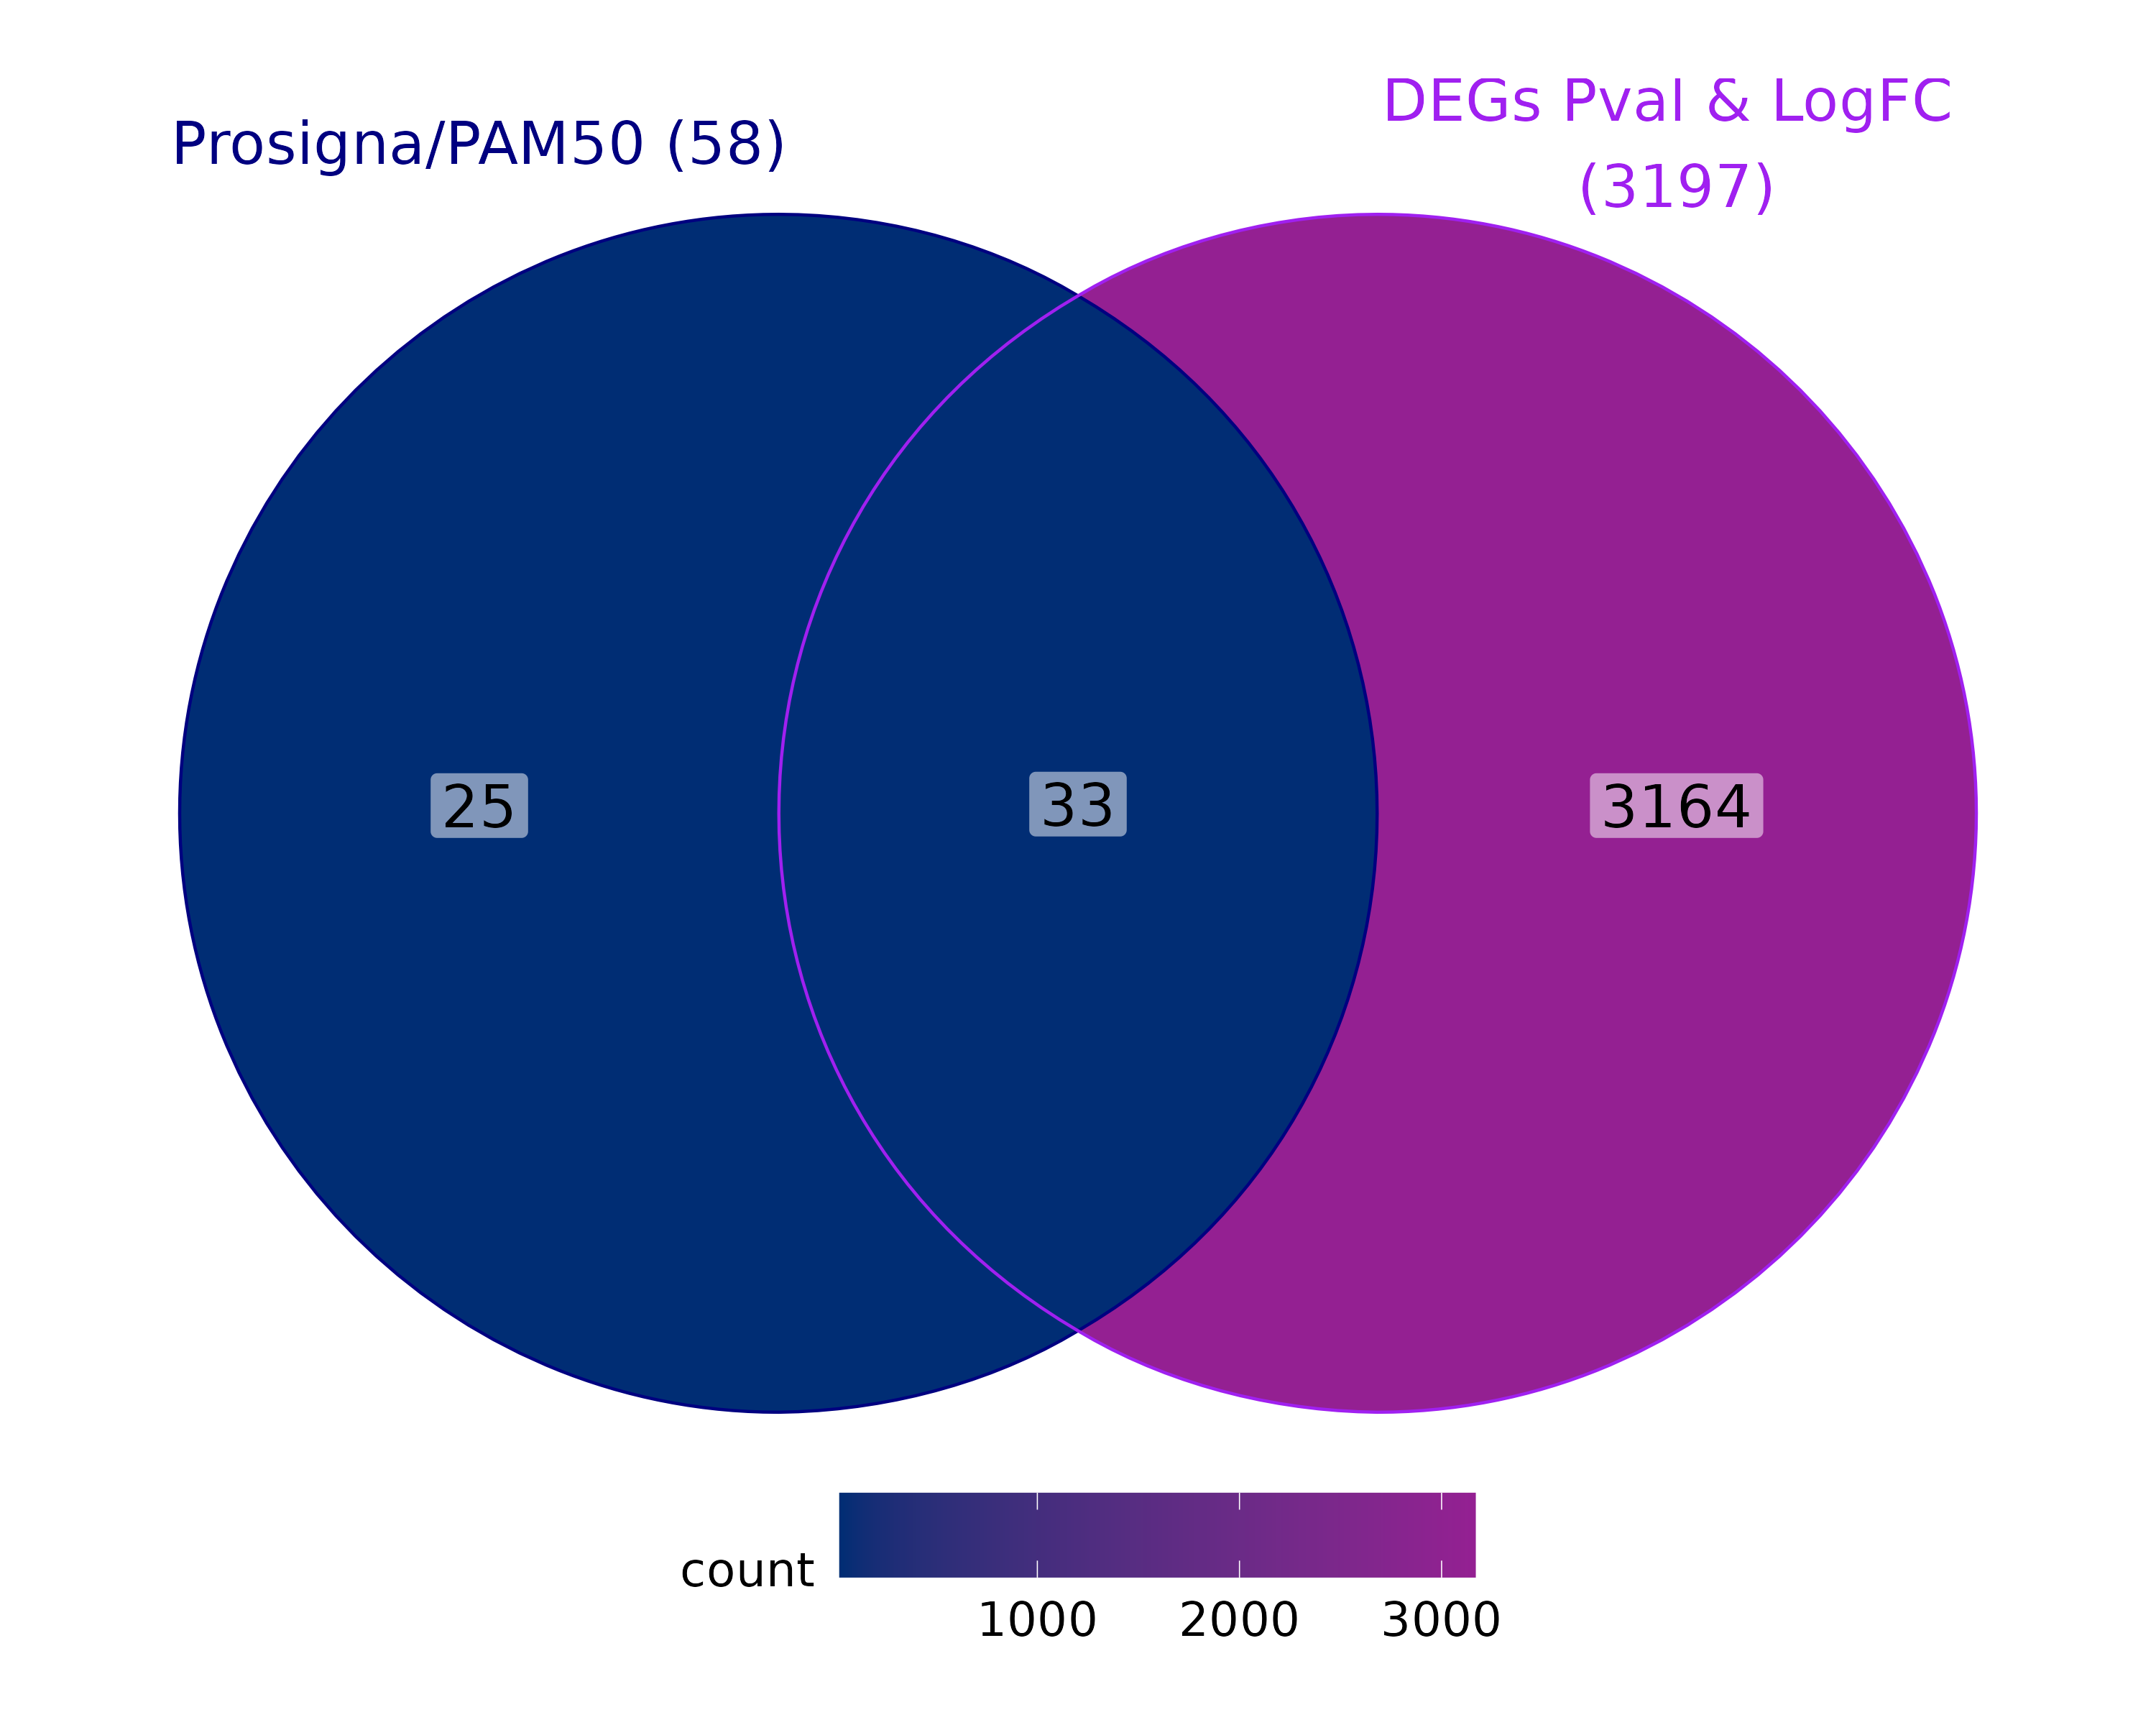
\includegraphics[width=0.5\textwidth]{../figures/Chapter_4/Venn_Prosig_PAM5_Ours.png}}
\subfloat[]{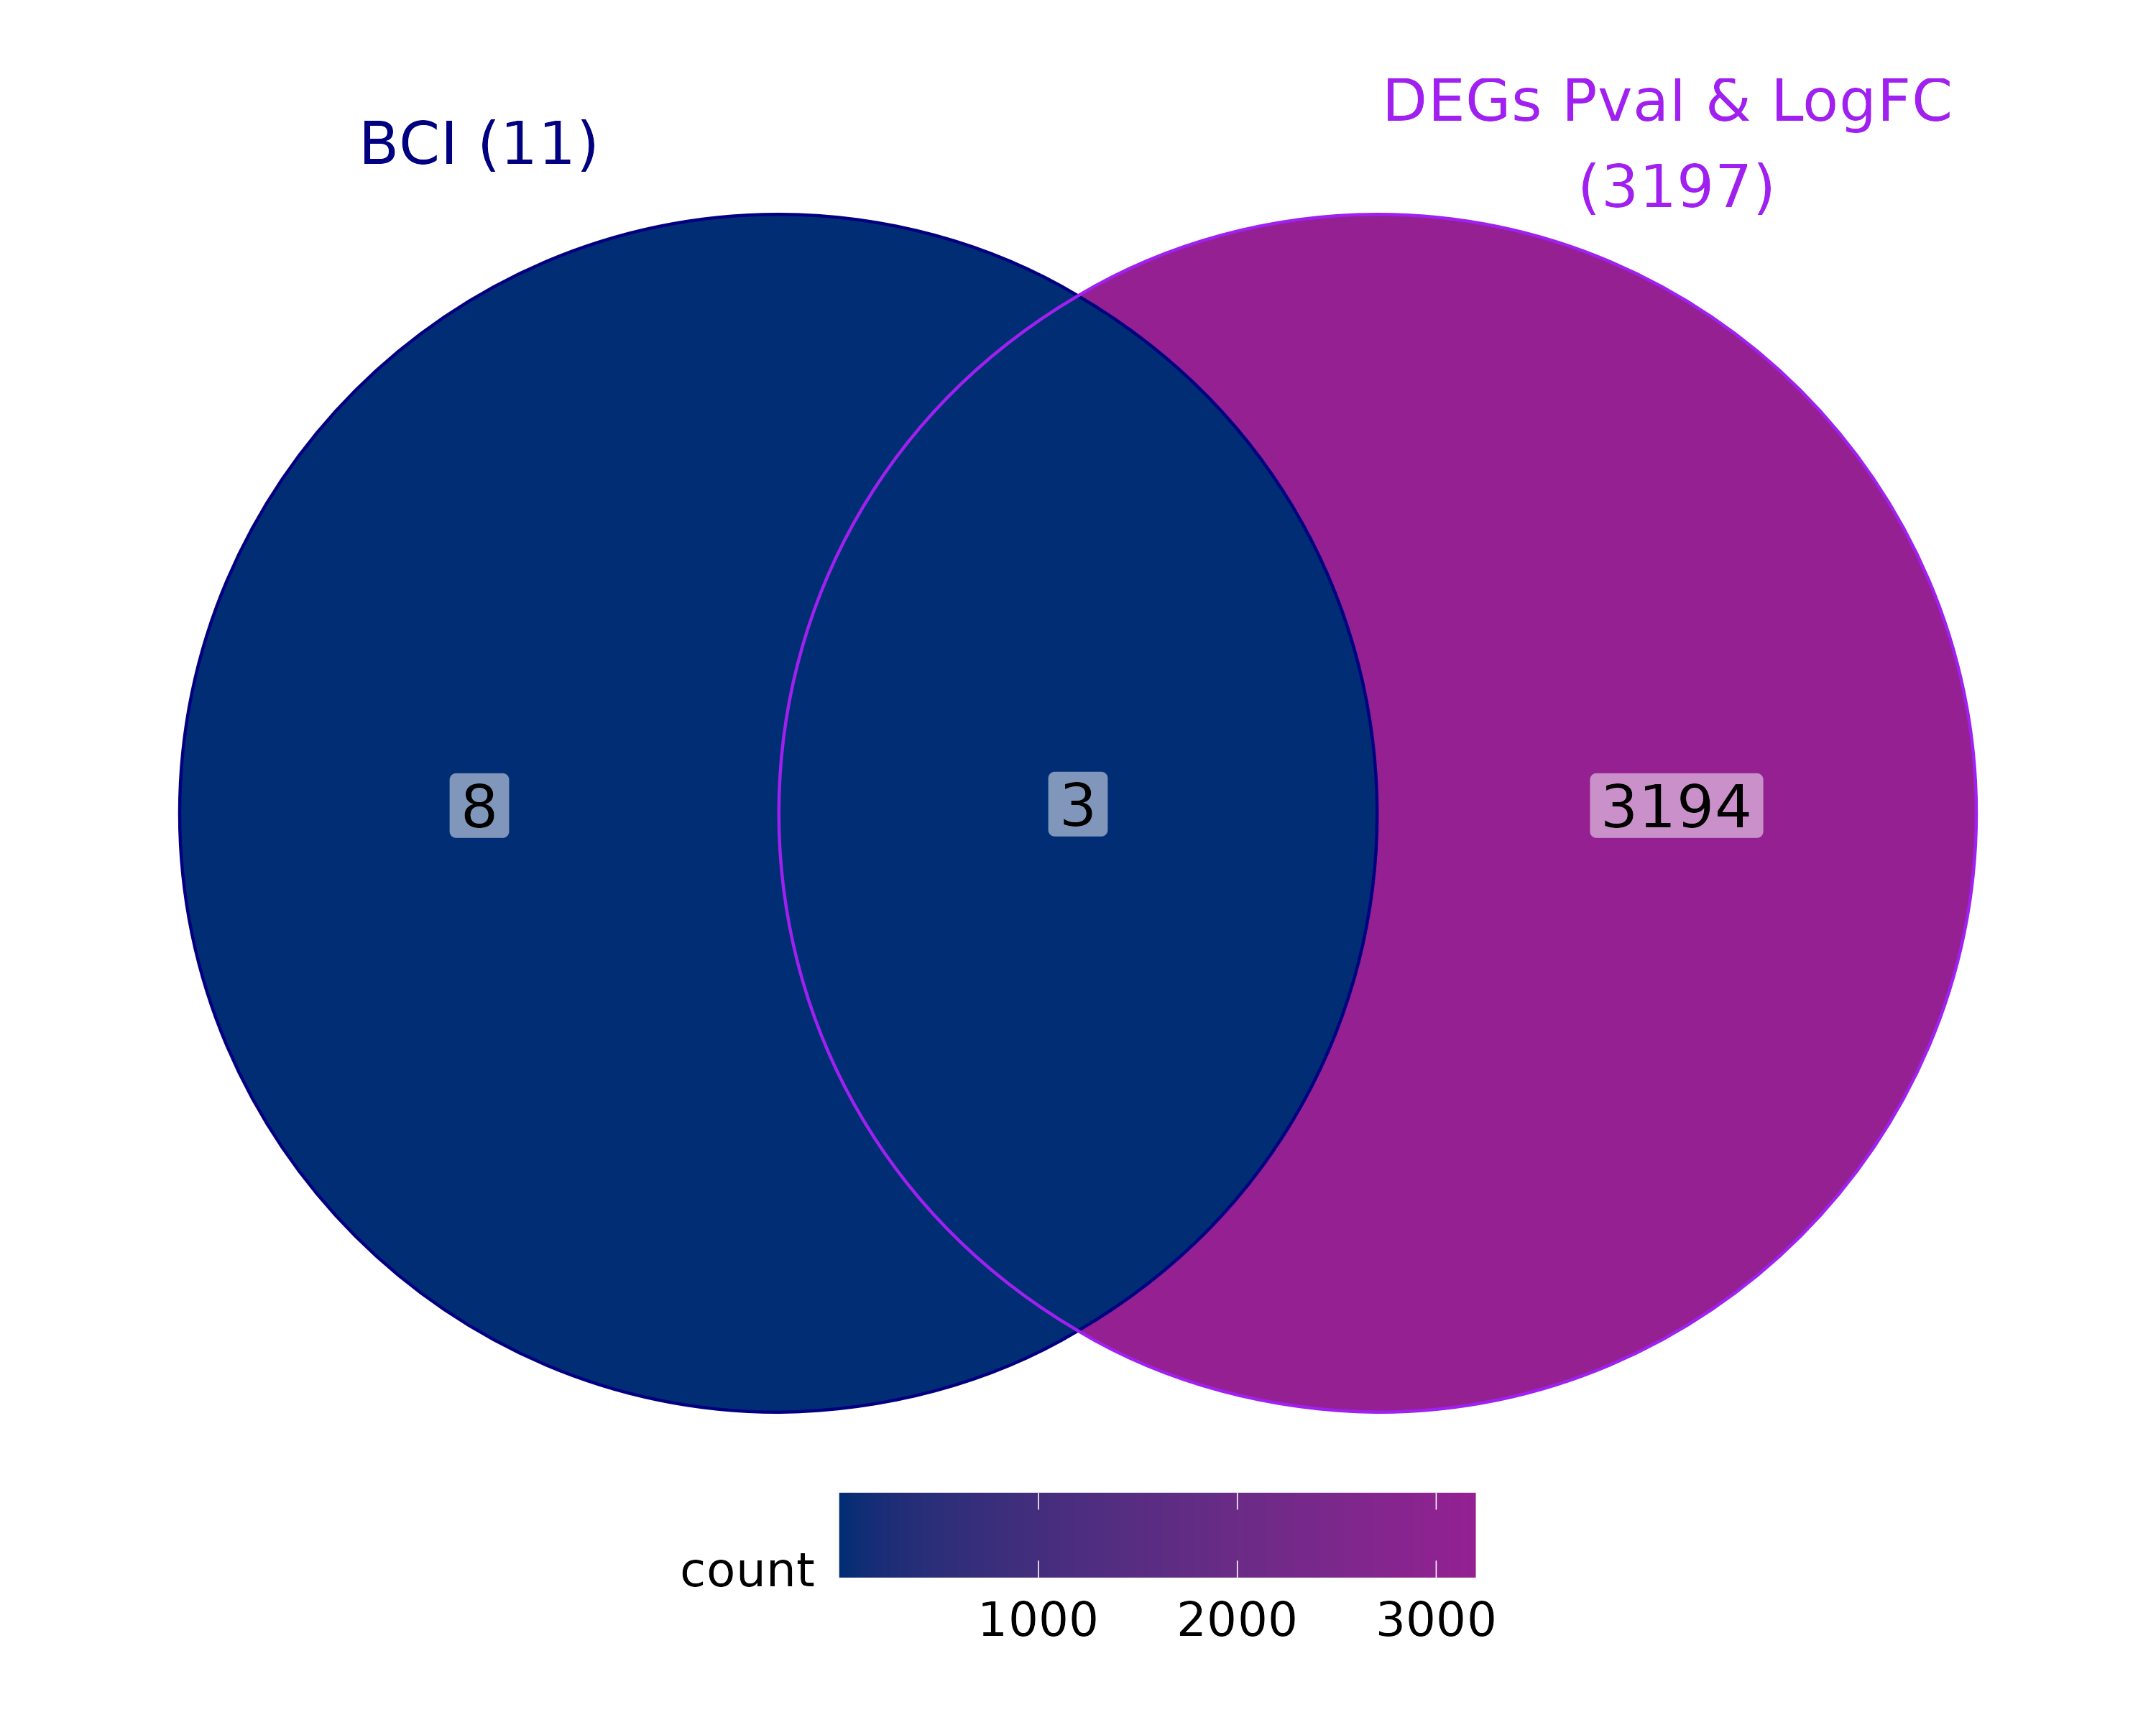
\includegraphics[width=0.5\textwidth]{../figures/Chapter_4/Venn_BCI_Ours.png}}

\subfloat[]{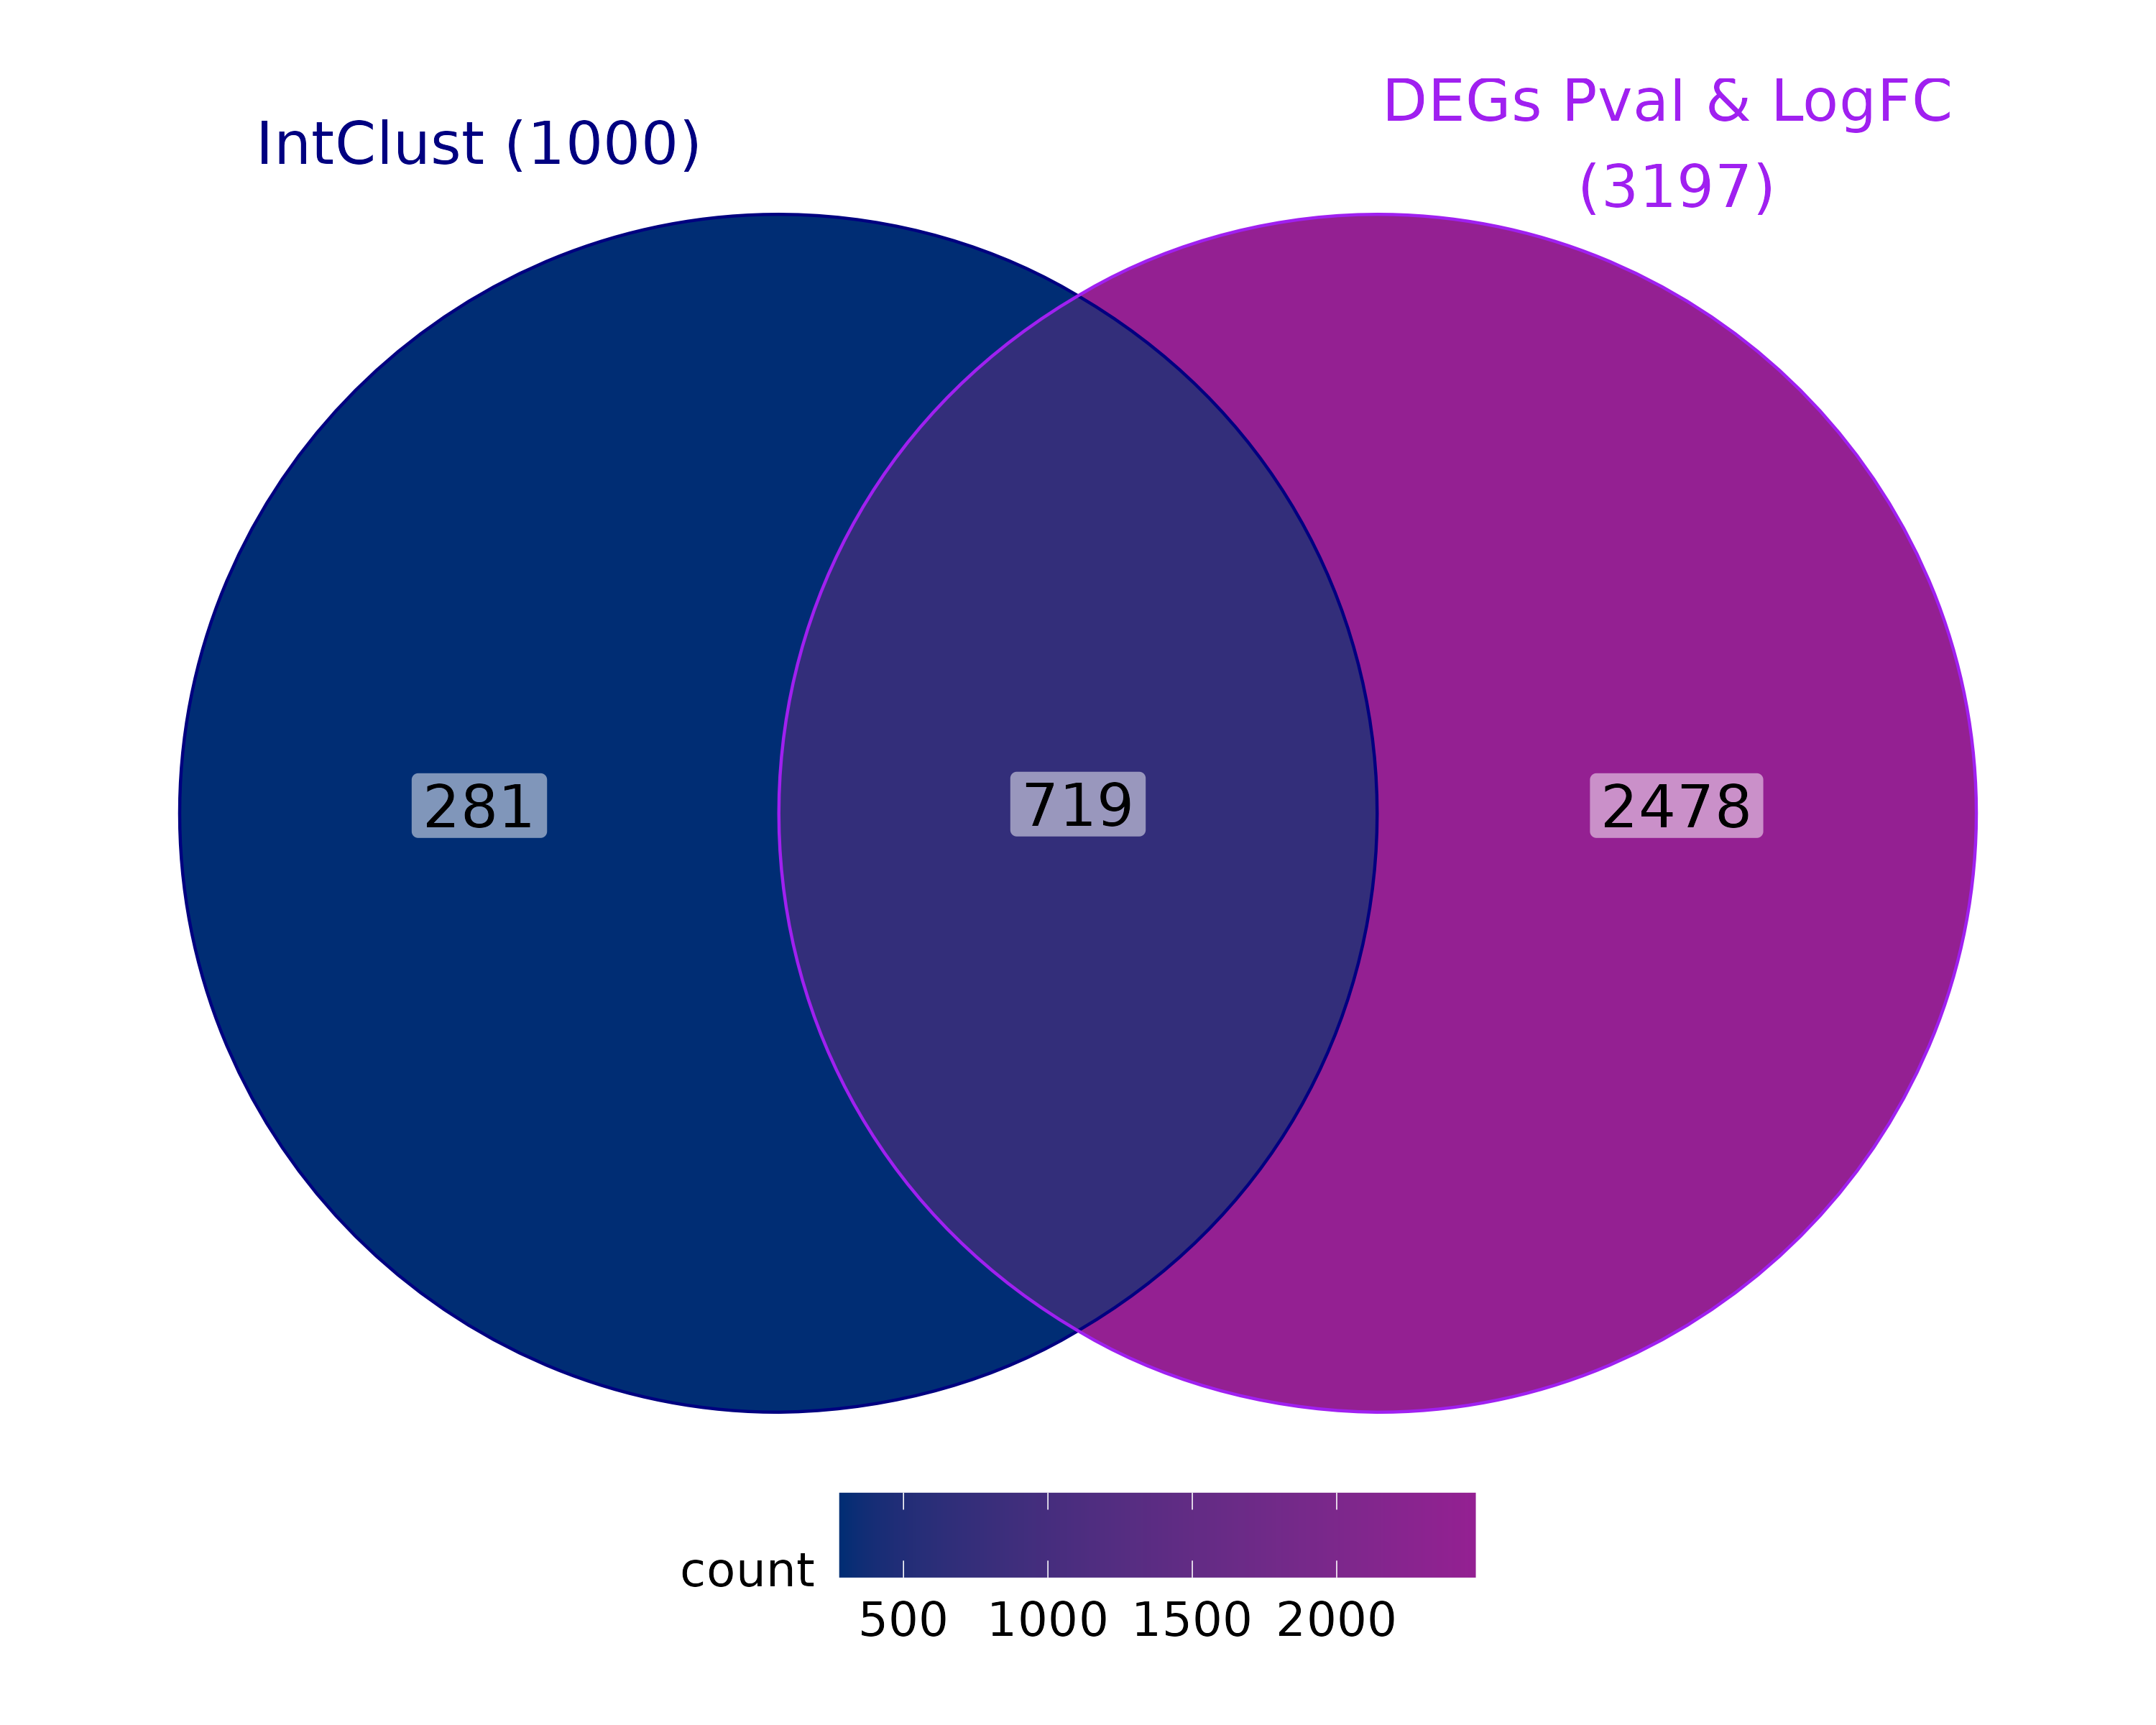
\includegraphics[width=.5\textwidth]{../figures/Chapter_4/Venn_IC_Ours.png}}
\subfloat[]{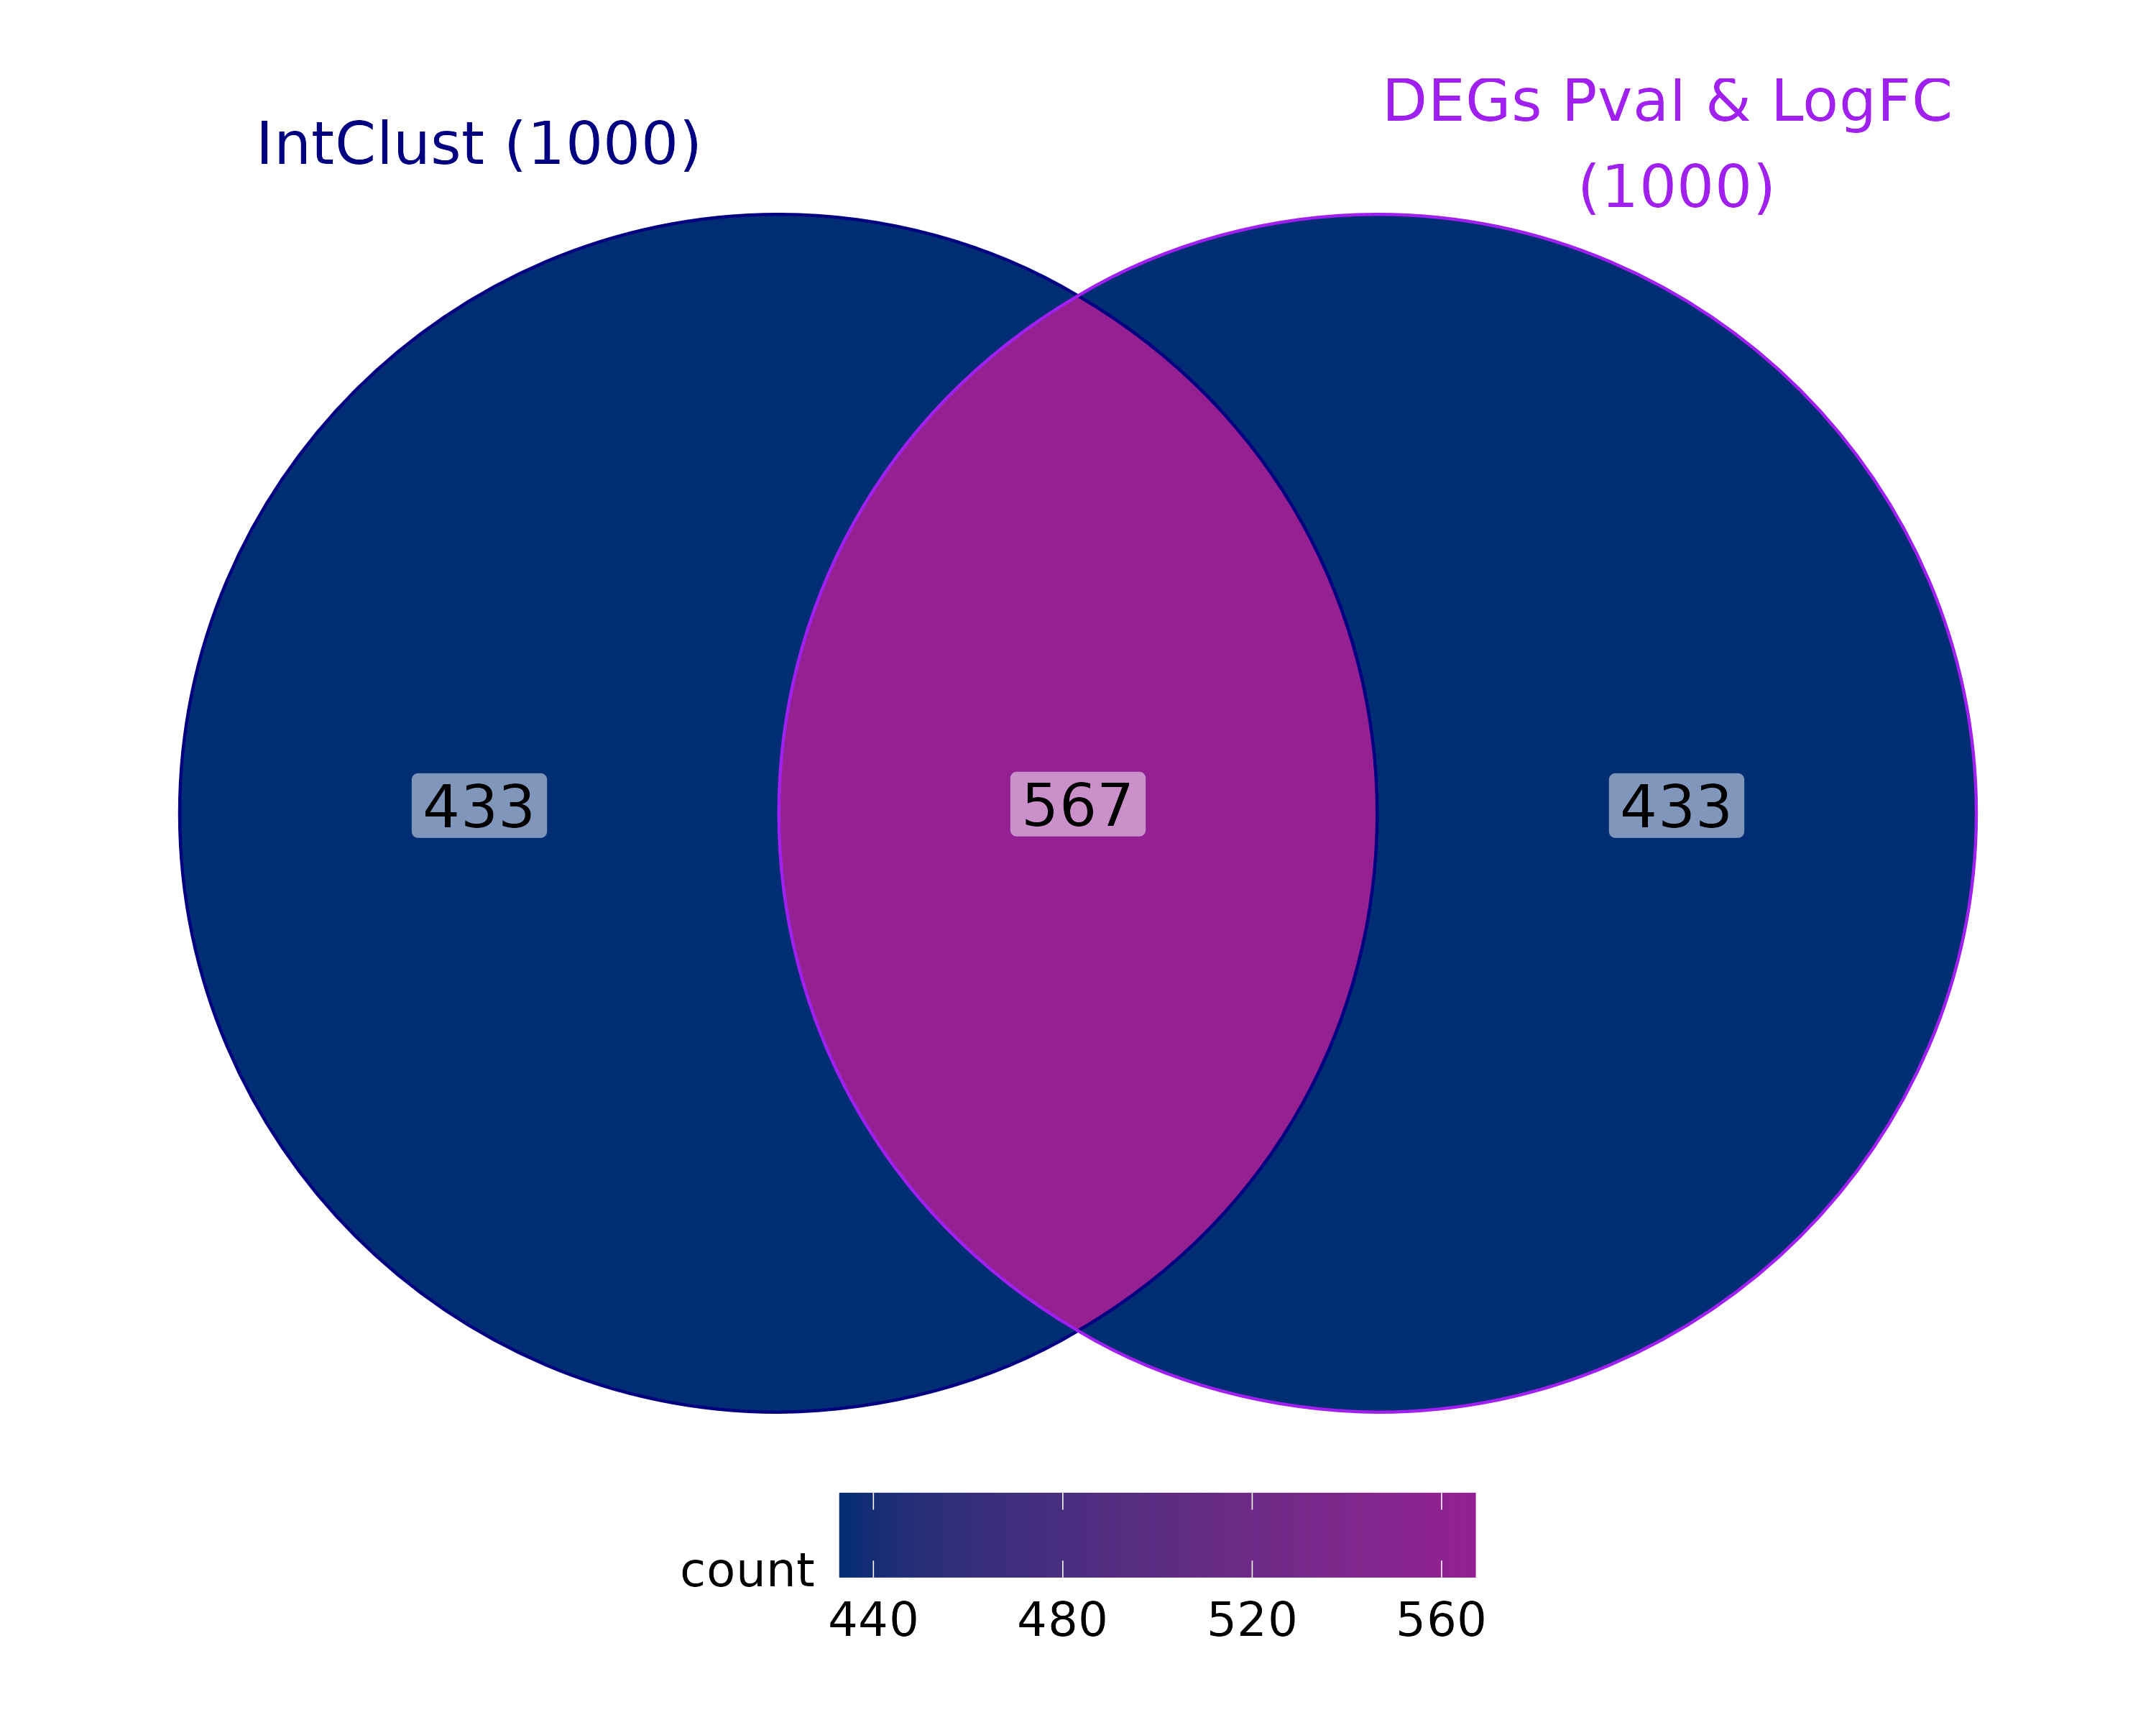
\includegraphics[width=.5\textwidth]{../figures/Chapter_4/Venn_IC_Ours_1000.png}}
\caption[Venn diagram showing gene set congruence between ModLim5 differentially expressed genes and prognostic and predictive assay genes.]{Venn diagram showing gene set congruence between ModLim5 differentially expressed genes and prognostic and predictive assay genes. (A) OncoType DX, (B) MammaPrint, (C) Prosigna/PAM50, (D) BCI, (E) IntClust and (F) IntClust (bound to n = 1,000).}\label{lab}

\label{fig:lo}
\end{figure}

\newpage
Focusing on the congruence between the prognostic and predictive assays, OncoType DX, MammaPrint, Prosigna and BCI, and the ModLim5 gene set, it is observed that 11 out of 21, 28 out of 66, 33 out of 58, and 3 out of 8 genes, respectively, are present in the ModLim5 gene set. This modest overlap is expected for a number of reasons, primarily due to the difference in objectives of each study. While the prognostic and predictive assays contain genes identified as useful in stratifying patients based on survival outcome and/or response to therapy, the ModLim5 gene set comprises genes where the presence of a CNA influences gene expression. 

As expected over half of the IntClust differentially expressed gene set is present in the ModLim5 differentially expressed gene set (Figure \ref{fig:lo}E and F). Congruence between these gene sets was expected for a number of reasons, mainly that the IntClust gene set was also produced using the METABRIC CNA and gene expression data and although the authors used a different approach (ANOVA and the Kruskal-Wallis test), the idea was similar. Interestingly, 281 genes present in the IntClust gene set are not found to be differentially expressed in our analysis. Reasons for this include absence from dataset, difference in method, Kruskal-Wallis versus modified limma, and also the difference in thresholds applied, adjusted p-values versus adjusted p-values and log-fold change. Indeed when only the adjusted p-value threshold is applied in our DGEA, 13,806 genes are differentially expressed, with 954 IntClust genes overlapping. Overall this DGEA analysis identified an additional 2,478 genes whose expression is influenced by CNAs and which should be considered for further investigation as candidate biomarkers for breast cancer treatment and outcome.

\subsection{Conclusions}
The literature reports that CNAs can influence gene expression and that some genes are more affected by the presence of a CNA than others. Both CNA and gene expression data have been used, separately and in tandem, to form molecular classification and prognostic and predictive assays of genes known to display differential expression and correlate with survival.   

In this chapter we compared gene expression profiles between METABRIC patients stratified by similarity in survival profiles as derived by global and chromosome arm specific metrics, i.e. comparing patients in particular survival tree nodes of interest. Under selected thresholds, a number of genes are found to be up- or down-regulated between the survival tree nodes. Genes observed to be up-regulated in patients in survival tree nodes associated with poorer survival outcomes include UBE2C, CXCL10 and S100P, while genes observed to be down-regulated in patients in survival tree nodes associated with poorer survival outcomes include PIP, BCL2 and IRX2. In cancer, overexpression of UBE2C, CXCL10 and S100P has been shown to facilitate cell proliferation, tumour progression and invasion, and correlate with worse survival outcomes \citep{pmid21195708, pmid31067633, pmid33681290}. Similarly, underexpression of PIP, BCL2 and IRX2 can facilitate tumour invasion and is associated poorer survival outcomes and response to therapy \citep{pmid20664598, pmid26560478, pmid30555735}. 

To investigate the direct relationship of a gene's CNA state to the gene's expression, a modified limma pipeline was employed, comparing gene expression profiles across patients based on the CNA state for each gene. From this analysis, it is evident that a large number of genes have altered gene expression when there is a CNA present. As expected, genes containing an amplification were often seen to be up-regulated, while genes containing a deletion were often seen to be down-regulated. Overall, using specified thresholds and considering sample size restrictions, 1,104 genes were differentially expressed in the three-gene specification, ModLim3, and 3,197 genes were differentially expressed in the five-gene specification, ModLim5. 

A comparative study to explore the extent of overlap between the ModLim5 gene set and molecular classification, prognostic and predictive assays published in the literature indicated a moderate degree of congruence, identifying some of the same genes, but also identifying additional genes to be considered for further investigation as candidate biomarkers for breast cancer treatment and outcome.

The CNA data utilised up to this point is total CNA data. In the next chapter we will consider allele-specific data and explore how to accurately identify and characterise CNA changepoints in allele-specific copy number profiles of breast cancer patients.